\documentclass[11pt,DIV=15,BCOR=20mm]{scrbook}

% Import von Paketen und Optionen die das gesamte Dokument betreffen
% sind in myPreamble.sty ausgelagert.
\usepackage{myPreamble}
\makeglossaries
% Glossar Einträge:

\newglossaryentry{model}{
    name={Model},
    description={A model in machine learning or deep learning is a mathematical representation that captures the relationship between inputs and outputs in data.
    It is used to make predictions about new, unseen data by applying mathematical operations to the inputs.
    Deep learning models are a subset of parametric models in which the parameters are represented as weights in a neural network and are changed during training to reduce the discrepancy between expected and actual outcomes.
    Machine learning models include but are not limited to decision trees, logistic regression, random forests, and linear regression.
    Convolutional neural networks (CNNs), recurrent neural networks (RNNs), and autoencoders are a few examples of deep learning models \cite{parsons2021WhatMachineLearning}},
    plural={models}
}

\newglossaryentry{lvm}{
    name={Latent variable model},
    description={
        Latent variable models are a type of probabilistic model that use latent or hidden variables to explain the observed data. 
        They model the relationship between the observed data and the latent variables through a set of conditional probability distributions.
        The goal is often to use this joint distribution to make predictions or perform inferences about the data, which typically involves marginalizing over the latent variables. 
        This means integrating over all possible values of the latent variables to obtain the probability distribution of the observed data \cite{skrondal2007LatentVariableModelling, bishop1998latent}
    },
    plural={latent variable models}
}

\newglossaryentry{mc}{
    name={Markov chain},
    description={A Markov chain, also known as a Markov process, 
    represents a probabilistic model where the likelihood of an event occurring is determined 
    exclusively by the outcome of the preceding event in a series of potential occurrences \cite{gagniuc2017MarkovChainsTheory}
    },
    plural={Markov chains}
}

\newglossaryentry{oh}{
    name={One-Hot},
    description={A One-Hot vector is a binary vector used to represent categorical data in machine learning and deep learning algorithms.
    It is characterized by having exactly one element set to 1 (the "hot" element) and all other elements set to 0. 
    Suppose a dataset contains a "color" feature with three distinct categories: red, green, and blue. 
    Using one-hot encoding, a unique one-hot vector for each color would look like the following:\\
    Red: [1, 0, 0]\\
    Green: [0, 1, 0]\\
    Blue: [0, 0, 1]
    },
    plural={One-Hot}
}

\newglossaryentry{pd}{
    name={pandas},
    description={
        Pandas \cite{mckinney-proc-scipy-2010} is an open-source Python library that provides high-performance, easy-to-use data structures, and data analysis tools. 
        It is designed to facilitate data manipulation, cleaning, analysis, and visualization in Python
    },
    plural={pandas}
}

\newglossaryentry{gdpr}{
    name={GDPR}, 
    description={The General Data Protection Regulation (GDPR) \cite{european_commission_regulation_2016} is a data privacy and security law passed by the European Union, which imposes standards and potential penalties on organizations worldwide that handle data related to people within the European Union
    },
    % first={General Data Protection Regulation (GDPR)\glsadd{gdprg}}, 
    % plural={GDPR}
}

\newglossaryentry{gdpraccr}{
    type=\acronymtype, 
    name={GDPR}, 
    description={General Data Protection Regulation},
    first={General Data Protection Regulation (GDPR)\glsadd{gdpr}}, 
    see=[Glossary:]{gdpr}
}


% Akkronyme
\newacronym{smote}{SMOTE}{Synthetic Minority Oversampling Technique}
\newacronym{vgm}{VGM}{Variational Gaussian Mixture model}
\newacronym{cnn}{CNN}{Convolutional Neural Network}
\newacronym{rnn}{RNN}{Recurrent Neural Network}
\newacronym{lstm}{LSTM}{Long Short-Term Memory}
\newacronym{gru}{GRU}{Gated Recurrent Unit}
% \newacronym{gdpr}{GDPR}{General Data Protection Regulation}
\newacronym{vae}{VAE}{Variational Autoencoders}
\newacronym{pca}{PCA}{Principal Component Analysis}
\newacronym{kl}{KL}{Kullback-Leibler}
\newacronym{gan}{GAN}{Generative Adversarial Network}
\newacronym{mlp}{MLP}{Multilayer Perceptron}
\newacronym{relu}{ReLU}{Rectified Linear Activation Unit}
\newacronym{ddpm}{DDPM}{Denoising Diffusion Probabilistic Model}
\newacronym{cdf}{CDF}{Cumulative Density Function}
\newacronym{mse}{MSE}{Mean-Squared Error}
\newacronym{pcd}{PCD}{Pairwise Correlation Difference}
\newacronym{dp}{DP}{Differential Privacy}
\newacronym{pmse}{pMSE}{propensity Mean Squared Error}
\newacronym{rmse}{RMSE}{Root Mean Squared Error}
\newacronym{gmm}{GMM}{Gaussian Mixture Model}
\newacronym{nlp}{NLP}{Natural Language Processing}
\newacronym{gpu}{GPU}{Graphics Processing Unit}
\newacronym{bgm}{BGM}{Bayesian Gaussian Mixture Model}
\newacronym{dcr}{DCR}{Distance to Closest Record}
\newacronym{cpu}{CPU}{Central Processing Unit}
\newacronym{ft}{FT}{Feature Tokenization}
\newacronym{rq}{RQ}{Research Question}

\begin{document}
% --- TITELSEITE ---
\begin{titlepage}

	% Fehler "destination with the same identifier" unterdrücken...
  \setcounter{page}{-1}

	% Titelseite
	\begin{figure}[h]
		\begin{minipage}[b]{62mm}
			
\includegraphics[width=62mm]{images/unilogo}
		\end{minipage}
		\hspace{4cm}
		%\begin{minipage}[b]{59mm}
		%	\includegraphics[width=59mm]{images/minlogo}
		%\end{minipage}
	\end{figure}

	\vfill
	
	\begin{center}
		% Diplomarbeit 
		\noindent { \huge
			Master's Thesis \\
		}
		\vspace{14mm}
		% Titel
		\noindent \textbf{\huge
		  Diffusion based Tabular Data Synthesis
		}
		\vspace{60mm}	
	\end{center}
	
	\vfill
	
	\noindent \textbf{Sven Groen} \\
	\noindent \rule{\textwidth}{0.4mm} 
	\noindent{\textrm{Sven.Groen@studium.uni-hamburg.de}} \\
	\noindent{\textrm{Studiengang IT Management und Consulting}} \\
	\noindent{\textrm{Matr.-Nr. 7388105}} \\
	\begin{tabbing}
	\hspace{8em} \=  \kill
	Erstgutachter: \> Dr. Fabian Panse \\
	Zweitgutachter: \> Professor Dr. Wolfram Wingerath \\
	~ \\
	Abgabe: 23.06.2023
	\end{tabbing}

\end{titlepage}


% \phantomsection
% \addcontentsline{toc}{chapter}{Abstract}
\thispagestyle{empty}
\begin{center}
	\textbf{\LARGE Abstract}
\end{center}
The growing demand for data in machine learning and deep learning applications, combined with the difficulties in acquiring and gathering real-world data, has fueled the development of synthetic data generation techniques.
Synthetic data, which is artificially generated but modeled on real data, can address privacy constraints and provide a cost-effective alternative for various use-cases.
With diffusion models, a newly emerged data generation technique, the quality of synthetic images increased and outperformed state-of-the-art \gls{gan}-based solutions. 
Recently, TabDDPM, a generative diffusion model, outperformed \glspl{gan} on tabular data synthesis as well.
Synthesizing tabular data presents unique challenges due to the complexity of the underlying joint distributions between variables and the need to capture intricate relationships among features.
While \gls{gan} based solutions have been heavily explored in the literature, diffusion-based solutions are relatively new and unexplored.


This thesis investigates whether adapting different tabular processing mechanisms from the literature positively affects the diffusion model's generative capability by encoding the tabular data into a different data format that specifically addresses known challenges of tabular data.
By extending the existing tabular data generation pipeline of TabDDPM, various tabular encoding and decoding strategies are implemented.
It focuses on two tabular processing mechanisms that encode the data before training and revert it back after sampling synthetic data: a static embedding technique named \gls{ft} and a mode-specific-normalization encoding technique that makes use of a \gls{bgm}.
In addition to that, this study touches upon the effects of normalization and hyperparameter optimization on diffusion models for tabular data synthesis.
The extended pipeline was evaluated using a CatBoost-based machine learning efficacy evaluation, a similarity metric TabSynDex, covering multiple similarity factors, and an analysis of visualization of the synthetic data.


The results demonstrate the superiority of diffusion models over other generative techniques, such as \Glspl{gan} and \gls{vae}, in generating synthetic tabular data.
The addition of a \gls{bgm}-based processing mechanism improves the TabDDPM model's performance in machine learning scenarios, while the \gls{ft} approach fails to produce meaningful data. 
The importance of hyperparameter tuning and data normalization strategies is highlighted, as well as the need for visual evaluation to accurately assess synthetic data quality. 
The effect of tuning the hyperparameters toward the TabSynDex similarity metric is bigger on diffusion models than on non-diffusion models.
This indicates the diffusion models' flexibility to generate synthetic data to cater to the specific requirements of the intended use case.
Lastly, diffusion models were capable of producing synthetic data that is more non-differentiable from the real data compared to non-diffusion models, which was indicated by a non-zero \gls{pmse} score. 

\cleardoublepage 

% 
\chapter*{Acknowledgements}
\label{ch:Acknowledgements}
\thispagestyle{empty}
I would like to thank Dr. Fabian Panse for his time, support, and insights that helped me write this thesis.
My gratitude also goes to the authors of the Paper "TabDDPM: Modelling Tabular Data with Diffusion Models" \cite{kotelnikov2022TabDDPMModellingTabular},
Babenko, Rubachev, Baranchuk and Kotelnikov, whose work functioned as the baseline for my master thesis.
I specifically want to express my thanks to Mr. Akim Kotelnikov, who took the time to answer me multiple questions about their paper and software code.


\cleardoublepage
\newpage \thispagestyle{empty}
% \pagestyle{plain}
% VERZEICHNISSE (Inhaltsverzeichnis, Abkürzungen)
% Vorspann einleiten --> Seitennummerierung römisch
\frontmatter

% --- Inhaltsverzeichnis --- 

\renewcommand{\contentsname}%
  {Table of Contents}%

\tableofcontents
\cleardoublepage

% % Glossar Einträge:

\newglossaryentry{model}{
    name={Model},
    description={A model in machine learning or deep learning is a mathematical representation that captures the relationship between inputs and outputs in data.
    It is used to make predictions about new, unseen data by applying mathematical operations to the inputs.
    Deep learning models are a subset of parametric models in which the parameters are represented as weights in a neural network and are changed during training to reduce the discrepancy between expected and actual outcomes.
    Machine learning models include but are not limited to decision trees, logistic regression, random forests, and linear regression.
    Convolutional neural networks (CNNs), recurrent neural networks (RNNs), and autoencoders are a few examples of deep learning models \cite{parsons2021WhatMachineLearning}},
    plural={models}
}

\newglossaryentry{lvm}{
    name={Latent variable model},
    description={
        Latent variable models are a type of probabilistic model that use latent or hidden variables to explain the observed data. 
        They model the relationship between the observed data and the latent variables through a set of conditional probability distributions.
        The goal is often to use this joint distribution to make predictions or perform inferences about the data, which typically involves marginalizing over the latent variables. 
        This means integrating over all possible values of the latent variables to obtain the probability distribution of the observed data \cite{skrondal2007LatentVariableModelling, bishop1998latent}
    },
    plural={latent variable models}
}

\newglossaryentry{mc}{
    name={Markov chain},
    description={A Markov chain, also known as a Markov process, 
    represents a probabilistic model where the likelihood of an event occurring is determined 
    exclusively by the outcome of the preceding event in a series of potential occurrences \cite{gagniuc2017MarkovChainsTheory}
    },
    plural={Markov chains}
}

\newglossaryentry{oh}{
    name={One-Hot},
    description={A One-Hot vector is a binary vector used to represent categorical data in machine learning and deep learning algorithms.
    It is characterized by having exactly one element set to 1 (the "hot" element) and all other elements set to 0. 
    Suppose a dataset contains a "color" feature with three distinct categories: red, green, and blue. 
    Using one-hot encoding, a unique one-hot vector for each color would look like the following:\\
    Red: [1, 0, 0]\\
    Green: [0, 1, 0]\\
    Blue: [0, 0, 1]
    },
    plural={One-Hot}
}

\newglossaryentry{pd}{
    name={pandas},
    description={
        Pandas \cite{mckinney-proc-scipy-2010} is an open-source Python library that provides high-performance, easy-to-use data structures, and data analysis tools. 
        It is designed to facilitate data manipulation, cleaning, analysis, and visualization in Python
    },
    plural={pandas}
}

\newglossaryentry{gdpr}{
    name={GDPR}, 
    description={The General Data Protection Regulation (GDPR) \cite{european_commission_regulation_2016} is a data privacy and security law passed by the European Union, which imposes standards and potential penalties on organizations worldwide that handle data related to people within the European Union
    },
    % first={General Data Protection Regulation (GDPR)\glsadd{gdprg}}, 
    % plural={GDPR}
}

\newglossaryentry{gdpraccr}{
    type=\acronymtype, 
    name={GDPR}, 
    description={General Data Protection Regulation},
    first={General Data Protection Regulation (GDPR)\glsadd{gdpr}}, 
    see=[Glossary:]{gdpr}
}


% Akkronyme
\newacronym{smote}{SMOTE}{Synthetic Minority Oversampling Technique}
\newacronym{vgm}{VGM}{Variational Gaussian Mixture model}
\newacronym{cnn}{CNN}{Convolutional Neural Network}
\newacronym{rnn}{RNN}{Recurrent Neural Network}
\newacronym{lstm}{LSTM}{Long Short-Term Memory}
\newacronym{gru}{GRU}{Gated Recurrent Unit}
% \newacronym{gdpr}{GDPR}{General Data Protection Regulation}
\newacronym{vae}{VAE}{Variational Autoencoders}
\newacronym{pca}{PCA}{Principal Component Analysis}
\newacronym{kl}{KL}{Kullback-Leibler}
\newacronym{gan}{GAN}{Generative Adversarial Network}
\newacronym{mlp}{MLP}{Multilayer Perceptron}
\newacronym{relu}{ReLU}{Rectified Linear Activation Unit}
\newacronym{ddpm}{DDPM}{Denoising Diffusion Probabilistic Model}
\newacronym{cdf}{CDF}{Cumulative Density Function}
\newacronym{mse}{MSE}{Mean-Squared Error}
\newacronym{pcd}{PCD}{Pairwise Correlation Difference}
\newacronym{dp}{DP}{Differential Privacy}
\newacronym{pmse}{pMSE}{propensity Mean Squared Error}
\newacronym{rmse}{RMSE}{Root Mean Squared Error}
\newacronym{gmm}{GMM}{Gaussian Mixture Model}
\newacronym{nlp}{NLP}{Natural Language Processing}
\newacronym{gpu}{GPU}{Graphics Processing Unit}
\newacronym{bgm}{BGM}{Bayesian Gaussian Mixture Model}
\newacronym{dcr}{DCR}{Distance to Closest Record}
\newacronym{cpu}{CPU}{Central Processing Unit}
\newacronym{ft}{FT}{Feature Tokenization}
\newacronym{rq}{RQ}{Research Question}
%\printglossaries[type=\acronymtype, title=Abkurzungsverzeichnis]
%\abbreviationsname[Abkürzungsverzeichnis]
\printglossary[type=main, title={Glossary}]
\printglossary[type=acronym, title={List of Abbreviations}]

%\printglossaries

%\let\cleardoublepage\clearpage % löscht die leere seite
\cleardoublepage
\phantomsection
% --- Figurenverzeichnis und Tabellenverzeichnis ---
\addcontentsline{toc}{chapter}{\listfigurename} % damit es in Inhaltsverzeichnis kommt
\listoffigures
%\let\cleardoublepage\clearpage % löscht die leere seite
\cleardoublepage
\phantomsection
\addcontentsline{toc}{chapter}{\listtablename}% damit es in Inhaltsverzeichnis kommt
\listoftables
\cleardoublepage
%\let\cleardoublepage\clearpage

% Hauptteil einleiten --> Seitennummerierung wieder arabisch
\mainmatter

% --- Hauptteil ---


\chapter{Introduction}
\label{ch:introduction}

\section{Problem Statement and Motivation} 
\label{ch:intro-problemStatement}

- success of DNNs \cite{borisov2022DeepNeuralNetworks}
- deployment of data-driven application requires solving 3 challenges (inference, data generation & interpretability) \cite{borisov2022DeepNeuralNetworks} (Focus on data generation)
- inference is most crucial but needs preprocessed training data with good quality --> data generation to address challenges (missing values, rebalancing, etc) \cite{borisov2022DeepNeuralNetworks}
- it might be simply impossible to use the actual data due to privacy concerns \cite{borisov2022DeepNeuralNetworks}

% For what do we need data? --> data is used everywhere
% Problems of real data (scarcity, privacy, etc.)
% What is synthetic data in 1 sentence
% What is special about tabular data
% use cases of synthetic data (privacy, scalability, availability, etc.)
% Why to use diffusion for synthetic data generation


% Motivation: Diffusion Probabilistic Models
% GAN's very successful for tabular data synthesis (plateau reached?)
% Diffusion beat GAN's in image synthesis (why not for tabular data?)
% first research shows that diffusion is better than GAN's for tabular data
% several improvements had been done to GAN's but not yet for Diffusion models
% Question arises: Can improvements from GAN's be transferred to Diffusion models?

\section{Goals and Research Questions}
\label{ch:intro-goals}

% Goals: extend the existing code base for special data preprocessing, statistical similarity (and maybe U-Net architecture)
% Goals: analysis on how to improve a Diffusion model for tabular data synthesis

% Research Questions:
% 1. does preprocessing the data into a specific format improve the results?
% 2. how good is diffusion for tabular data synthesis in terms of statistical similarity?
% 3. does a special tabular data synthesis metric improve the results when used for hyperparameter optimization?

% (Wenn Zeit übrig ist):
% 3. does using a U-Net architecture improve the results? (maybe)
% 4. Can the similarity score be incorporated into the loss function? (maybe)


\section{Proceeeding}
\label{ch:intro-proceeeding}

% Proceeeding:
% Literature research on Diffusion models and GAN's
% --> What has been done, what has worked, what has not worked, what can be used for diffusion models
% --> decide which improvements are most promising and will be implemented
% Use existing code base for Diffusion models
% --> implement improvements proposed for GAN's and apply to them Diffusion
% --> train different Diffusion versions
% --> Evaluate the results with additional meassures (statistical meassures)
% Compare the results with the current state of the art
% Analyze the results and draw conclusions (what works, what doesn't work, what can be improved)


\section{Contributions}
\label{ch:intro-contributions}
%Problem Statement: Clearly state the research problem being addressed and explain why it is important. Provide a detailed definition of the problem and explain how it relates to the field of tabular data synthesis.

%Research Objectives: Define the specific research objectives of the thesis and explain how they contribute to the overall research problem.

%Research Methodology: Describe the methodology used to address the research problem, including the techniques and tools used, the data sources used, and the data analysis techniques used.

\subsection{Data Preprocessing}
\label{ch:intro-contributions-dataPreprocessing}

% Data preprocessing is a crucial step in data synthesis
% Use special preprocessing for tabular data
% flexible and extendable preprocessing module inside the current implementation

\subsection{Model Architecture} % maybe 
\label{ch:intro-contributions-modelArchitecture}

% Current Diffusion models are based on simple MLP's
% U-Net architecture is used for image synthesis
% Use U-Net architecture for tabular data synthesis?

\subsection{Extended Evaluation}
\label{ch:intro-contributions-extendedEvaluation}

% Current work focuses on Machine learning efficiency
% Add additional evaluation metrics
% "Similarity Score" used from Master thesis paper that aggregates several metrics


\section{Outline}
\label{ch:intro-outline}

\chapter{Preliminaries}
\label{ch:preliminaries}

\section{Tabular Data}
\label{ch:preliminaries-dataSynthesis-tabularData}

Tabular data is one of the most common forms of structured data \cite{hernandez2022SyntheticDataGeneration} used to store, classify and share information \cite{pilaluisa2022ContextualWordEmbeddings}.
A table is made up of individual cell entries stored in rows and columns.
Rows can be seen as unique data points, and columns as their different features \cite{borisov2022DeepNeuralNetworks, yoon2020VIMEExtendingSuccess}.
This format is the most common way to maintain massive databases \cite{esmaeilpour2022BidiscriminatorGANTabular, yoon2020VIMEExtendingSuccess}, and is crucial for applications that store heterogeneous information such as demographics, medical or financial information \cite{borisov2022DeepNeuralNetworks, yoon2020VIMEExtendingSuccess}.
Tabular data consists of multiple attribute types, such as categorical or continuous data types \cite{borisov2022DeepNeuralNetworks}.
From a statistical perspective, quantitative and qualitative variables are to be differentiated \cite{lane2003IntroductionStatistics}.
Quantitative variables are variables that can be measured numerically and express a specific quantity or amount. 
Qualitative variables cannot be measured numerically but describe qualities or characteristics that do not have any ordering  \cite{lane2003IntroductionStatistics}. 
These variables are divided into categories or groups based on shared attributes. 
The categories are usually non-numerical and consist of words or labels, such as gender (\textit{male}, \textit{female}) or hair color (\textit{blonde}, \textit{brunette}, \textit{red}, etc.) and may be assigned to numbers.

Quantitative variables can be further subdivided into continuous or discrete variables.
Continuous variables can take on an infinite number of values within a specific range. 
These variables are often measured on a continuous scale, can have decimal or fractional parts, and are stored as a numerical data type \cite{lane2003IntroductionStatistics, lederrey2022DATGANIntegratingExperta}.
Discrete variables are also numbers, but they can only have a specific and limited number of unique values within a certain range. 
They are usually expressed as whole natural numbers (or integers) and are commonly used for counting or listing items. \cite{lane2003IntroductionStatistics}.

Qualitative variables are often called categorical values and can be further classified into binary or nominal types \cite{lane2003IntroductionStatistics}.
Binary variables have only two possible outcomes (\eg booleans with \textit{True} or \textit{False}), while nominal variables consist of at least three distinct values that do not follow a specific order \cite{lederrey2022DATGANIntegratingExperta, lane2003IntroductionStatistics}.

\newpage
This work adapts the formal definition of a table from \cite{xu2019ModelingTabularData}:

\begin{displayquote}
A table \textbf{$T$} contains $N_q$ qualitative (categorical) columns $\{Q_1, \dots, Q_{N_q}\}$ and $N_p$ quantitative columns $\{P_1, \dots, P_{N_p}\}$, 
where the quantitative columns consist of both continuous and discrete variables. 
Each column is considered to be a random variable. 
These random variables follow an unknown joint distribution $\mathbb{P}(Q_{1:N_q}, P_{1:N_p})$. 
One row $r_j = \{q_{1,j}, \dots, q_{N_q,j}, p_{1,j}, \dots, p_{N_p,j}\}$, $j \in \{1, \dots, n\}$, is one observation from the joint distribution.
\end{displayquote}

The term "table" as described in this definition aligns with the concept of a single "table" or "relation" as described in the classical relational model \cite{codd1970RelationalModelData} commonly used in modern relational databases \cite{w.eembley2009RelationalModel}.
Essentially, this definition takes a probabilistic view of the table in a relational database.
Rather than viewing the data within the table as static or independent values, it perceives them as elements derived from an unseen, underlying probability distribution.
This is an important perspective for statistical analysis and machine learning tasks on database content.

\cite{codd1970RelationalModelData}

For consistency and simplicity, this thesis will further refer to qualitative columns as \textit{categorical} and to quantitative columns as \textit{continuous} or \textit{numerical}. 
Discrete values are not separately mentioned but should be considered included in \textit{continuous}/\textit{numerical} columns.

It is also possible that tabular data contains other particular data types like dates or timestamps, which often include information on the specific time a datapoint was recorded \cite{hernandez2022SyntheticDataGeneration}.
This kind of tabular data can be considered dynamic tabular data, where individual records, \ie rows, can be dependent on each other, also known as a multivariate time series \cite{padhi2021TabularTransformersModeling}.
In static tabular data, on the other hand, the individual rows are independent \cite{padhi2021TabularTransformersModeling}.
Hence, the order of rows and columns does not carry any meaning \cite{somepalli2021SAINTImprovedNeural}.
However, the individual values in one cell may vary well depending on the values of another cell \cite{lederrey2022DATGANIntegratingExperta}.
An example of such an interdependency could occur in a demographics table, where an individual's legal status may depend on their age, 
for example, a person under 18 years of age could be considered a minor and has different legal rights and responsibilities than an adult.

The authors of \cite{borisov2022DeepNeuralNetworks} identify four possible challenges when working with tabular data in a learning context.
The first challenge identified is the "low-quality" of the data \cite[p. 4]{borisov2022DeepNeuralNetworks}. 
\textcite{borisov2022DeepNeuralNetworks} identified common data quality issues from the literature, which include missing values, data noise, extreme data points, inconsistencies, class imbalances, or high dimensionality of the data after preprocessing.

Secondly the "missing or complex irregular spatial dependencies" of tabular data \cite[p. 4]{borisov2022DeepNeuralNetworks}. 
Other common data formats like images or audio are homogeneous, meaning that they consist of only one feature type \cite{borisov2022DeepNeuralNetworks}.
Since tabular data consists of multiple features made up of a mixture of categorical and numerical values, it is a heterogeneous data format with data points as rows and features as columns \cite{borisov2022DeepNeuralNetworks}.
This format presents particular challenges for neural networks when working with tabular data, as the correlations between features are often weaker due to the absence of spatial or semantic relationships commonly found in image or text data \cite{borisov2022DeepNeuralNetworks, yoon2020VIMEExtendingSuccess}.

The third challenge is the "dependency on preprocessing" \cite[p. 4]{borisov2022DeepNeuralNetworks}. 
\cite{borisov2022DeepNeuralNetworks} highlights the importance of a preprocessing and an explicit feature construction step that is necessary when working with tabular data in a deep learning context.
This preprocessing step is crucial since it not only strongly influences the performance of deep learning models \cite{gorishniy2022EmbeddingsNumericalFeatures}, it also introduces new challenges. 
Depending on the preprocessing strategy (\autoref{sec:preprocessing}), it is possible to create a very sparse feature matrix, construct a synthetic ordinal ordering of a nominal variable, or lose some information during the conversion of the data \cite{borisov2022DeepNeuralNetworks}.

The last and fourth challenge concerns the "importance of single features" \cite[p. 4]{borisov2022DeepNeuralNetworks}. 
In homogeneous data, multiple features need to change in order for the class of the data to be changed. 
For heterogeneous tabular data, a small change in one feature variable can already alter the class of the row. 
\cite{borisov2022DeepNeuralNetworks} illustrates this with the example of an image, where multiple pixels (\ie features) need to change in a coordinated manner in order to change the content (\ie class) of the image from a dog to a cat.
For tabular data, a single change in a cell can change the prediction of a predictive model \cite{borisov2022DeepNeuralNetworks}. 
Consider a model that has to predict whether an individual's income is higher or lower than US\$ 50.000 per year \cite{Dua:2019} based on the demographic information of that individual.
Switching an individual's "education" value from "Preschool" to "Doctorate" would likely cause the prediction to change from "<=50K" to ">50K".


\subsection{Tabular Data Preprocessing}
\label{sec:preprocessing}

Different data types can and should be processed into a meaningful format to be useful for deep learning models in different ways \cite{fan2020RelationalDataSynthesisa, lederrey2022DATGANIntegratingExperta}.
That is usually the first step before working with the data on any task \cite{izonin2022TwoStepDataNormalization}.
\cite{garcia2016BigDataPreprocessing} states, that data preprocessing itself consists of multiple different tasks: data cleaning, data normalization, data transformation, data integration, missing value imputation and noise identification.
While each of the preprocessing tasks in itself is important, 
\cite{fitkov-norris2012EvaluatingImpactCategorical} and \cite{gorishniy2022EmbeddingsNumericalFeatures} showed that a proper transformation of categorical and numerical entries respectively can have a significant influence on a deep learning model's performance.
\cite{xu2019ModelingTabularData} showed the importance of normalization for synthetic tabular data generation.
Since the focus of this work is on tabular data and its synthesis, the following section will highlight the most important tabular data transformation and normalization approaches.

\subsubsection{Data Transformation}
\label{sec:dataTransformation}

\textcite[p. 5]{borisov2022DeepNeuralNetworks} introduced a taxonomy for data transformation methods and subdivides the existing approaches into "Single-Dimensional Encodings" and "Multi-Dimensional Encodings".
The goal is to transform the different values a column can take and transform them into a different (numeric) representation so that it can be processed by a deep learning model.

\textbf{Single-Dimensional Encodings:}
Single-Dimensional encoding techniques encode each cell independently \cite{borisov2022DeepNeuralNetworks}.
The following approaches are common techniques to encode a categorical column entry, usually in a text format, into a numerical format.
In ordinal- (or label-) encoding, a simple mapping from each category to a numeric value occurs. 
While this introduces a synthetic ordering of potentially unordered categories, \gls{oh} encoding overcomes this issue by introducing a new vector with the length of all possible values a categorical column can take.
All values in this vector are assigned to zero except one entry which represents the category that should be encoded, which is set to one.
However, this approach can lead to high-dimensionality feature vectors if the cardinality of the unique categories in categorical columns is large.
Binary encoding tries to reduce the dimensionality by setting the vector length to a maximum of $log(c)$ for $c$ unique categorical values in a column \cite{borisov2022DeepNeuralNetworks}.
Each possible value is mapped to a number like in ordinal-encoding, starting at 0, but the number is represented as a binary vector.
As an example, the categorical values \{\textit{Germany}, \textit{USA}, \textit{France}\} would be represented as binary values \{(0,1), (1,0), (1,1)\}. 
While representing \textit{France} in a one-hot-encoding creates the vector (0,0,1) of length three, binary encoding encodes the same information into the vector (1,1) of length two, reducing the overall dimensionality of produces encodings.
The leave-one-out encoding technique is an approach to encode a categorical column based on the target column in a machine learning scenario \cite{borisov2022DeepNeuralNetworks}. 
A categorical entry is replaced by the mean of the target variable of all rows where the same category is present, excluding the target value of the to be encoded value.
Lastly, a hash-based approach is worth mentioning, where a deterministic hash function transforms each category into a numerical form \cite{borisov2022DeepNeuralNetworks}.

Numerical data, such as integers or floating point numbers, can often be used directly in deep learning models without undergoing a special encoding process. 
This is because deep learning algorithms are designed to handle numerical data and can learn patterns and relationships within the data without the need for additional encoding.
However, \cite{gorishniy2022EmbeddingsNumericalFeatures} has shown that in some cases, encoding numerical data can improve the performance of deep learning models. 
Encoding numerical data can be achieved through various methods such as normalization, discretization, or using embeddings.

%Die beiden abschnitte auslagern in eigenen abschnitt? (GGF nur embeddings auslagern?)
Discretization techniques transform numerical features to categorical features, hence, quantitative data into qualitative data \cite{garcia2016BigDataPreprocessing}. 
\cite{dougherty1995SupervisedUnsupervisedDiscretization} gives an overview of classical discretization techniques, such as equal interval width binning, where the continuous values are divided and assigned to a certain amount of bins.
Researchers from NVIDIA \cite{dong2022GeneratingSyntheticData} have recently put forth a new method, introducing a tokenizer designed specifically for handling tabular data with floating-point numbers.
This tokenizer converts float numbers into a sequence of token IDs \cite{dong2022GeneratingSyntheticData}.

In embedding techniques, values that should be encoded (\eg words or tabular cell entries) are mapped into a vector representation. 
This vector of real numbers tries to capture "semantic regularities in vector spaces" \cite[p. 2]{pilaluisa2022ContextualWordEmbeddings}.
The goal of embeddings is to create a vector space, in which semantically similar values are also numerically similar \cite{pilaluisa2022ContextualWordEmbeddings}.
It can be differentiated between static embeddings and contextualized embeddings. 
While the former embedding technique always provides the identical numerical representation for an input value, the latter embedding technique changes the vector representation of a value based on its surrounding context \cite{pilaluisa2022ContextualWordEmbeddings}.
This is especially important in the \gls{nlp} domain, where contextual embeddings have led to state-of-the-art improvements \cite{pilaluisa2022ContextualWordEmbeddings}.
Homonyms or polysemic words like \textit{bat} or \textit{second} are words that carry multiple different meanings and their semantic meaning therefore can change with the context they are used in.
Hence, the contextualized embedding vector of the word \textit{second} in the context of \textit{Time} (\eg \textit{"it took me 3 seconds"}) should be different from the one where \textit{second} is used in the context of \textit{Competition} (\eg \textit{"he achieved the second place}").
Contextualized embeddings have to be learned during some form of (pre-) training \cite{devlin2019BERTPretrainingDeep, iida2021TABBIEPretrainedRepresentations, deng2021TURLTableUnderstanding}. 
Static embedding techniques, such as Word2Vec \cite{mikolov2013DistributedRepresentationsWords} are learned as well.
However, a static embedding would always create the same vector representation for \textit{second}, while a contextualized embedding vector would be different, depending on the context the word \textit{second} is used in.
Using the embedding layers to get a vector representation without learning is also possible, which can be seen as a "feature tokenization" \cite{zheng2022DiffusionModelsMissing, gorishniy2021RevisitingDeepLearning}.
However, semantic similarity in a vector space cannot be achieved without any learning, so this embedding technique is more similar to a discretization/tokenization technique.

% [TODO: Insert example for single-dim encoding in tabular data] --> warum nochmal?

\textbf{Multi-Dimensional Encodings:}
Multi-Dimensional encoding techniques focus on encoding an entire record (or table-row) into another representation \cite{borisov2022DeepNeuralNetworks}.
The VIME framework \cite{yoon2020VIMEExtendingSuccess} uses a multilayer perceptron as an encoder that encodes a tabular input row into a latent representation, 
similar to the encoder of famous (variational-) auto-encoders \cite{kingma2013AutoEncodingVariationalBayes} architectures.
This latent representation is, like in embeddings, a learned representation that is learned through self-supervised learning tasks, feature vector estimation and mask vector estimation \cite{yoon2020VIMEExtendingSuccess}.
\cite{borisov2022DeepNeuralNetworks} also lists other multi-dimensional encoding techniques, such as the works of \cite{zhu2021ConvertingTabularData} and \cite{sun2019supertml}.
Both architectures transform tabular data into an image-like format in order to make use of \glspl{cnn}.


\subsubsection{Data Normalization and Standardization}
\label{sec:dataNormalization} 

Normalization and standardization techniques are applied to numerical columns and scale the values so that their distribution is adjusted \cite{garcia2016BigDataPreprocessing}.
This is especially important in tabular data, where numerical features are likely to have a different scale, \eg a column \textit{Age} could have a range of 1 to 100 and a column \textit{Capital-gain} could have a range from 0 to 100.000, as it is the adult income dataset \cite{Dua:2019} (\autoref{ch:methods-datasets}).
Normalization allows to scale each column a similar range (usually 0 to 1, or -1 to 1) while maintaining the overall distribution of each column \cite{izonin2022TwoStepDataNormalization}.
Standardization on the hand rescales the data so it follows a normal distribution with mean 0 and standard deviation 1 \cite{scikit-learndevelopers2023PreprocessingData}.
Standardization and Normalization of values is especially important if the data will be used in a machine learning context, where machine learning models might behave unexpectedly if 
the features do not look similar to a Gaussian distribution or are not ranged between 0 and 1 \cite{scikit-learn, scikit-learndevelopers2023PreprocessingData}.
Through this data rescaling, the sensitivity of models to large values is reduced and the generalizability is increased \cite{izonin2022TwoStepDataNormalization}.
Two popular standardization and normalization approaches are the standard and the min-max scaler, respectively.
The standard scaler standardizes a feature value $x_i$ according to the mean and standard distribution of the feature column so that it follows a normal distribution \cite{garcia2016BigDataPreprocessing, izonin2022TwoStepDataNormalization}.
It can be defined as $x' = \frac{x_i-mean(x)}{std(x)}$, with $x'$ as the standardized $x_i$ value \cite{izonin2022TwoStepDataNormalization}.
The min-max scaler is a normalization technique that makes use of the maximum and minimum of each feature column and scales the values accordingly.
It is defined as $x' = \frac{x_i - min(x)}{max(x) - min(x)}$ \cite{izonin2022TwoStepDataNormalization}.
While the standard scaler is usually used for data that follows a Gaussian normal distribution, the min-max scaler is better suited for arbitrary distributions, however, it is quite affected by outliers \cite{choudhury2020FeatureScalingEffect}.
A more complex normalization technique addresses the problem that numeric values in tabular data can follow distributions in a more complex way than just a simple Gaussian normal distribution \cite{zhao2022CTABGANEnhancingTabular, xu2019ModelingTabularData}.
\textcite{xu2019ModelingTabularData} introduces mode-specific normalization which models complex distributions with multiple simple Gaussian distributions.
The authors define the mode-specific normalization technique in following way \cite[p. 3-4]{xu2019ModelingTabularData}:

\begin{enumerate}
    \item For each continuos column $C_i$, estimate the number of modes $m_i$ by using a \gls{vgm} \cite{bishop2006PatternRecognitionMachine}. 
    For example, in \autoref{fig:mode-specific-normalization} the \gls{vgm} estimates $m_i=3$, referred to as $\eta_1$, $\eta_2$ and $\eta_3$. 
    The learned Gaussian mixture is  
    $\mathbb{P}_{C_i}(c_{i,j})=\sum_{k=1}^{3}\mu_k\mathcal{N}(c_{i,j};\eta_k, \sigma_k)$
    with $\mu_k$ and $\sigma_k$ as the weight and the standard deviation of a mode respectively.
    $\mu_k$ can also be understood as the proportion of the overall data that comes from the $kth$ mode, essentially measuring the likelihood, a randomly selected datapoint from the overall dataset comes from the $kth$ determined gaussian distribution.
    \item For each $c_{i,j}$ the probability is calculated of $c_{i,j}$ coming from each mode. 
    In \autoref{fig:mode-specific-normalization}, $p_1$, $p_2$ and $p_3$ denote the probability densities, calculated as $p_k=\mu_k\mathcal{N}(c_{i,j};\eta_k;\sigma_k)$.
    \item Given $p_1$, $p_2$ and $p_3$ for $c_{i,j}$ one mode is sampled and used to normalize the value. 
    In the example of \autoref{fig:mode-specific-normalization}, $p_3$ is most likely and is sampled.
    The mode selection for $c_{i,j}$ is represented as a \gls{oh} vector $\beta_{i,j}=[0,0,1]$ indicating that the third mode has been sampled.
    The actual value $c_{i,j}$ is normalized as $\alpha_{i,j}=\frac{c_{i,j}-\eta_3}{4\sigma_3}$, according to the mean and standard deviation of $p_3$. 
\end{enumerate}

The normalized representation $r$ of $c_{i,j}$ will be the concatenation of $\alpha_{i,j}$ and $\beta_{i,j}$: 
$$r=\alpha_{i,j}\oplus\beta_{i,j}$$

For example, given $\alpha_{i,j}=0.4$ and $\beta_{i,j}=[0,0,1]$, the normalized representation would be $r=[0.4,0,0,1]$

% include image from paper
\begin{figure}[h]
    \centering
    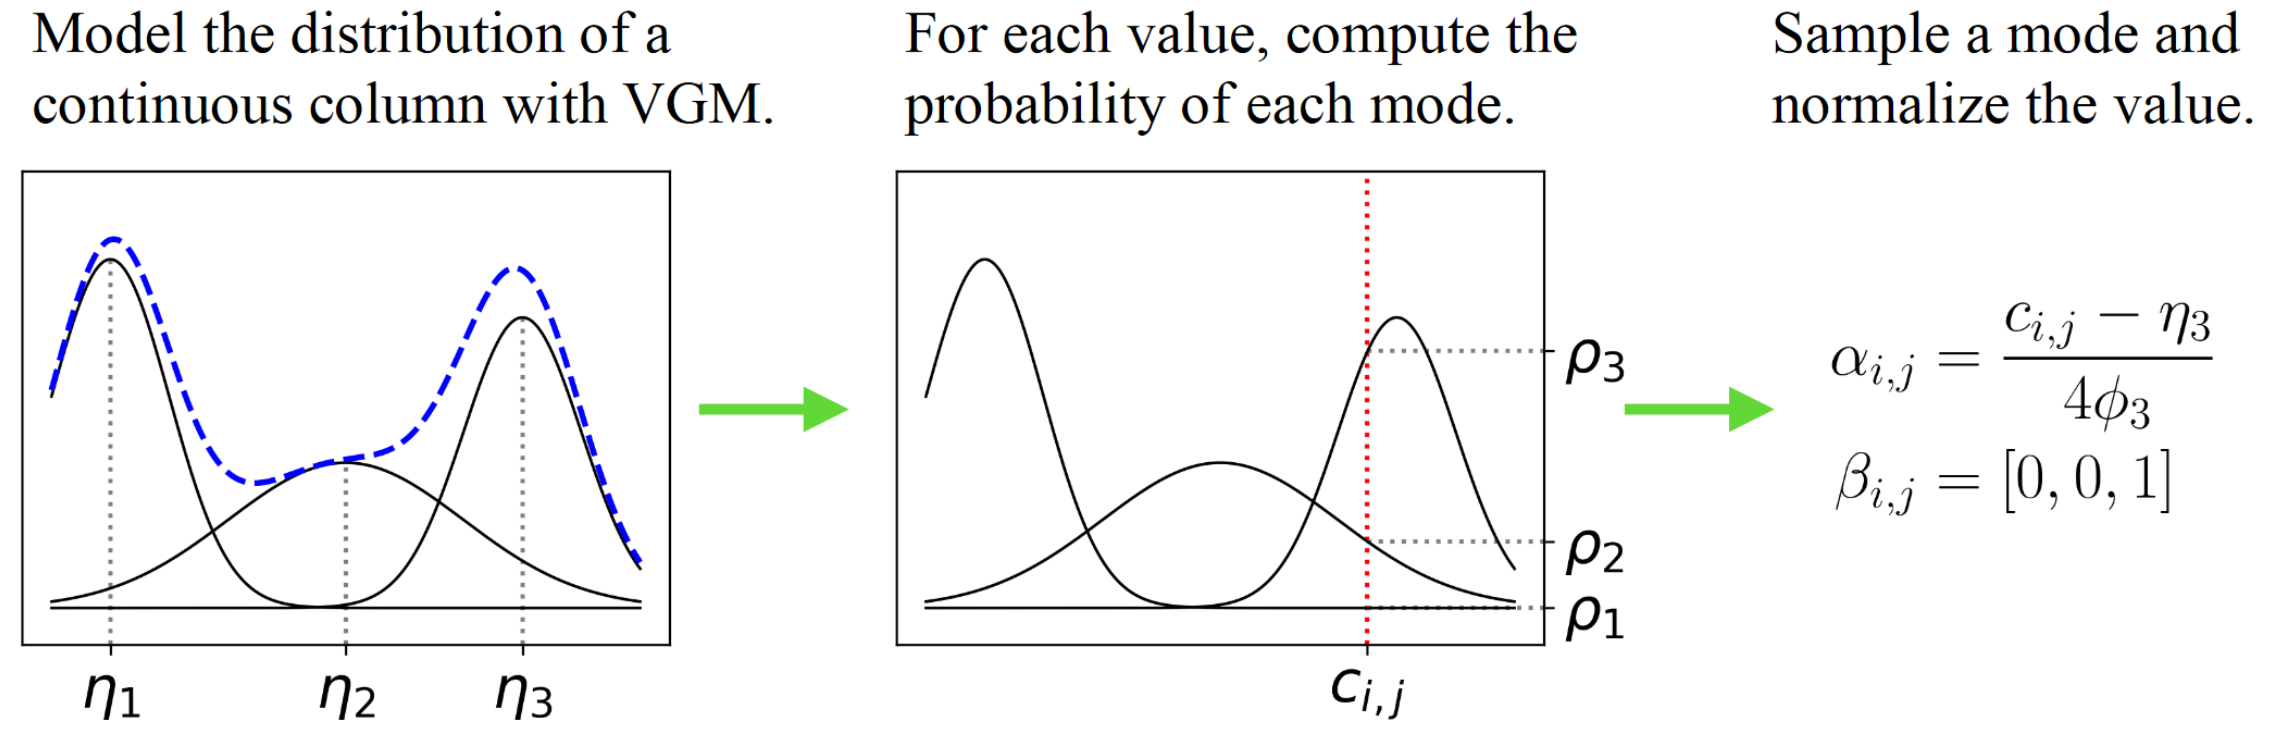
\includegraphics[width=0.8\textwidth]{images/mode-normalization.png}
    \caption[Mode-Specific Normalization]{An example of mode-specific normalization \cite[Figure 1, p. 4]{xu2019ModelingTabularData}}
    \label{fig:mode-specific-normalization}
\end{figure}

Another approach to standardize the range of a column between 0 and 1 is a Quantile-transformation, which is a non-linear transformation \cite{scikit-learndevelopers2023PreprocessingData, kotelnikov2022TabDDPMModellingTabular}.
The Quantile-transformation allows the mapping of all values of a random variable into a desired output distribution, such as the uniform or normal distribution, 
using the quantile function on the inverse cumulative distribution of the random variable. 
This transformation preserves the rank order of the values but distorts correlations and distances within and across features \cite{scikit-learndevelopers2023PreprocessingData}.


%-------------------------------------------------------------------------
\section{Data Synthesis}
\label{ch:preliminaries-dataSynthesis}

\subsection{Synthetic Data}
\label{ch:preliminaries-dataSynthesis-syntheticData}
Synthetic data can be defined as "(...) artificially generated data, that are modeled on real data, with the same structure and properties as the original data (...)" \cite[p. 2]{kaloskampis2020SyntheticDataCivil} 
but without containing any actual specific information or entries of the actual real data. 
While first synthetic data approaches \cite{gelman1992InferenceIterativeSimulation} focused on imputation techniques to generate synthetic data, the advent of deep learning has led to the topic gaining importance \cite{kowalczyk2022TaxonomyUseSynthetic, kaloskampis2020SyntheticDataCivil}.
Acquiring and collecting real data can be costly \cite{panova2022HowSyntheticData} or may simply not be possible due to the sensitivity of the data (\eg medical records) \cite{esteban2017RealvaluedMedicalTimea} or due to regulatory restrictions, such as the \gls{gdpr} \glsadd{gdpraccr} \cite{european_commission_regulation_2016}.
Synthetic data on the other hand is, compared to real data, cheap to generate \cite{leminh2021AirGenGANbasedSynthetica}, fulfils regulatory and privacy constraints \cite{zhao2022CTABGANEnhancingTabular} and can substitute real data in software development for testing \cite{whiting2008CreatingRealisticScenariobased} or machine learning training \cite{panova2022HowSyntheticData}.
Hence, synthetic data could be used as an alternative to real data in various use cases.
Access to data is still one of the biggest bottlenecks when developing machine learning or deep learning models \cite{fan2020RelationalDataSynthesisa}.
Synthetic data could be used to increase the data quality, by rebalancing skewed dataset \cite{zhao2022CTABGANEnhancingTabular} 
or increasing the dataset size as additional training data or in combination with the real data \cite{leminh2021AirGenGANbasedSynthetica, kim2021OCTGANNeuralODEbased}.
Synthetic data can also be used in situations where working with the real data is not possible, due to privacy or availability reasons \cite{9034117, whiting2008CreatingRealisticScenariobased}.
In software development, high-quality test data is crucial for development but challenging and time-consuming to generate \cite{whiting2008CreatingRealisticScenariobased}.
Developers' time to create such datasets is usually scarce and it might be the case that developers do not even have permission to see the data, due to its sensitivity \cite{whiting2008CreatingRealisticScenariobased}.
A synthetic data generation model would possibly allow developers to generate test data with predefined characteristics without it being restricted in any form.


\subsection{Synthetic Tabular Data Generation}
\label{sec: synthetic tabular data generation}

Generative models have recently received a lot of attention, thanks to their impressive results in generating a variety of data formats, 
such as images \cite{ho2020DenoisingDiffusionProbabilistic, dhariwal2021DiffusionModelsBeat, rombach2022HighResolutionImageSynthesis}, videos \cite{ho2022VideoDiffusionModels, runwayGen1Runway}, text \cite{radfordImprovingLanguageUnderstanding, openai2022ChatGPTOptimizingLanguage}, or music \cite{agostinelli2023MusicLMGeneratingMusic, Forsgren_Martiros_2022}.

While synthetic data generation can be applied to various types of data, generating synthetic tabular data is challenging due to the complexity of the underlying joint distributions between variables \cite{borisov2022DeepNeuralNetworks}.
This works formal definition of the tabular data generation is adapted from \cite[p. 2]{xu2019ModelingTabularData} and expands the definition of a table from \autoref{ch:preliminaries-dataSynthesis-tabularData}:

\begin{displayquote}
    A data synthesizer $G$ is trained on a table $T$ and then used to generate a synthetic table $T_{syn}$. % Vllt die definition einer tabelle nach oben packen und von oben übernehmen?
    $T$ is partitioned into a training set $T_{train}$ and test set $T_{test}$. 
    The synthesizer $G$ is trained on $T_{train}$ and afterwards used to sample independently individual rows to create $T_{syn}$.
    Finally, the similarity of $T_{syn}$ to $T_{test}$ is evaluated using a selected similarity evaluation technique.
\end{displayquote}

The synthetic dataset $T_{syn}$ should exhibit a similar relationship with the test dataset partition $T_{test}$ 
as the one found between the training dataset partition $T_{train}$ and $T_{test}$. 
This is crucial for maintaining the underlying structure and properties of the original data.
The primary objective for the generative model $G$ is to create $T_{syn}$ in such a way that it appears to originate from the same joint distribution as the complete dataset $T$. 
This ensures that the synthetic data maintains the essential characteristics of the original data.
Importantly, $T_{syn}$ is not directly compared to $T_{train}$, because the purpose of generating $T_{syn}$ is not to merely replicate $T_{train}$,
but to create a new dataset that preserves the inherent relationships and properties of the original data.

During the generation of synthetic tabular data, there are two competing objectives: high data utility and low disclosure risk.
Data utility is concerned with how well the synthetic data accurately reflects the real data in terms of its underlying patterns and relationships.
Low disclosure risk on the other hand is concerned with the preservation of privacy and confidentiality of the information in the real training dataset $T_{train}$ \cite{little2021GenerativeAdversarialNetworksa}. 

Tabular data synthesis approaches can be divided into process- and data-driven methods \cite{goncalves2020GenerationEvaluationSynthetic}.
Process-driven models focus on simulating real-world processes and gather data during that simulation to create the synthetic dataset \cite{goncalves2020GenerationEvaluationSynthetic, kowalczyk2022TaxonomyUseSynthetic}.
On the other hand, data-driven approaches aim to generate synthetic data based on already existing real-world datasets \cite{goncalves2020GenerationEvaluationSynthetic, kowalczyk2022TaxonomyUseSynthetic}.
This can be achieved by augmenting the existing dataset, \ie applying transformations to the existing individual datapoints to generate new datapoints \cite{kowalczyk2022TaxonomyUseSynthetic}.
Another technique to generate synthetic data is to simply sample from the individual feature distributions of a dataset to create new synthetic data \cite{kowalczyk2022TaxonomyUseSynthetic}.
Lastly, machine learning and deep learning algorithms can be used to learn the underlying joint distributions of the real data to generate new synthetic data \cite{kowalczyk2022TaxonomyUseSynthetic}. 
%challanges
Compared to other data types, the synthesis of tabular data is especially challenging due to its heterogeneity, potential weak correlations among features and the dependency on preprocessing \cite{borisov2022DeepNeuralNetworks, yoon2020VIMEExtendingSuccess, gorishniy2022EmbeddingsNumericalFeatures}.
To create a realistic synthetic dataset, interdependencies that may exist between variables must be captured and 
it is possible that the model overfits on the training data and generalizes relationships between features that are only present in training but not in the test data \cite{lederrey2022DATGANIntegratingExperta}.
In addition to that, tabular data columns can follow complex distributions, which makes the synthesis challenging.
\textcite{zhao2022CTABGANEnhancingTabular} identified the following four properties of tabular data, one should consider when trying to synthesize tabular data:

\begin{enumerate}
    \item \textbf{Single Gaussian variables}: Data where its distribution follows a Gaussian distribution \cite{zhao2022CTABGANEnhancingTabular}.
    \item \textbf{Mixed data type variables}: A single column can contain a mix of continuous and categorical values. 
    For instance, a \textit{Loan} column could hold information about the size of an individual's loan.
    The values in this column are mostly positive float values but can also take the value \textit{$-1$} which indicates that this person did not get approved for a loan.
    Such a special categorical value in an otherwise purely numerical column needs to be considered when working with this column \cite{zhao2022CTABGANEnhancingTabular}.
    \item \textbf{Long tail distributions}: In real-world data, most data points may occur "near the initial value of a distribution and rare cases towards the end" \cite[p. 3]{zhao2022CTABGANEnhancingTabular}.
    This results in a tail-like distribution.
    The phenomenon of long-tail distribution is seen across a variety of applications including object detection, scene parsing, document processing, and item recommendation \cite{zhou2018DeepSuperclassLearning}.
    Capturing these long-tail distributions correctly during the synthesis is important, not only because they represent unique or rare scenarios that could be crucial for certain analysis tasks, but also because the minority classes in the tail collectively constitute a significant portion of the entire dataset \cite{zhou2018DeepSuperclassLearning}. 
    \item \textbf{Skewed multi-mode continuous variables}: Complex numerical distributions do not necessarily follow a single Gaussian distribution.
    It is possible for their distribution to consist of multiple unknown distributions that are potentially skewed as well. 
    Their conjunction as a whole makes up the complex distribution \cite{zhao2022CTABGANEnhancingTabular}, as it could be seen in the example of \autoref{fig:mode-specific-normalization}.
\end{enumerate}

A successful tabular data generator should be able to recreate such properties of real data in their synthetic data counterpart.


\section{Deep Learning Architectures}
\label{ch:preliminaries-deepLearningArchitectures}

Deep learning has rapidly become a dominant force in artificial intelligence, revolutionizing various fields including computer vision, \gls{nlp}, and generative modeling. 
Here, complex neural networks architectures emerged with multiple layers and complex interconnections.
These architectures have enabled the creation of highly accurate and efficient models that are capable of processing vast amounts of data from different modalities.

In recent years, this development of new deep-learning architectures has been a key area of research, leading to the creation of such powerful models.
This section will start with a high-level introduction into a neural network's most important architectural building blocks.
Afterwards, the most important deep learning model architectures for generating data are presented.

\subsection{Neural Networks}
\label{ch:preliminaries-deepLearningArchitectures-neuralNetworks}

The most basic neural network is called a perceptron \autoref{fig:perceptron} \cite{rosenblatt1958PerceptronProbabilisticModel}.
It consists of a single input layer that is connected to an output node.
Each input node is connected with the output node via weight edges.
For all inputs, the input value is multiplied by each respective weight.
The sum of all input-weights' multiplication serves as the input to an activation function, which is different depending on the task at hand.
The output is the prediction of the perceptron which is compared to the actual result, the label, and an error is calculated.
This error is later used to update the individual nodes' weights via backpropagation \cite{aggarwal2018NeuralNetworksDeep}.
The output of one node can also serve as the input to another node, so multiple layers of nodes are created.
This is referred to as a \gls{mlp} or feed-forward neural network as presented in \autoref{fig:mlp}, 
because the information flows forward from input through the multiple layers in the middle (also called hidden layers) to the output \cite{aggarwal2018NeuralNetworksDeep, Goodfellow-et-al-2016}.
An \gls{mlp} tries to approximate some function $f^*$ by defining a mapping $y=f(x;\theta)$ and learning the values of the parameters $\theta$ (\ie the weights) that best approximate $f^*$ \cite{Goodfellow-et-al-2016}.
A simple \gls{mlp} is already able to learn almost any function, which is why they are also considered to be universal function approximators \cite{aggarwal2018NeuralNetworksDeep, hornik1989MultilayerFeedforwardNetworks}.


\begin{figure}
    \begin{subfigure}{0.8\textwidth}
      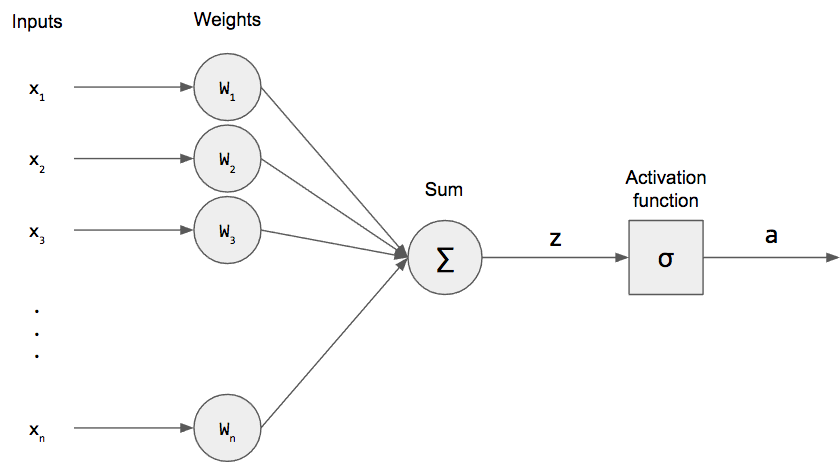
\includegraphics[width=\linewidth]{images/perceptron.png}
      \caption[Perceptron]{Perceptron} \label{fig:perceptron}
    \end{subfigure}%
    \hspace*{\fill}   % maximize separation between the subfigures
    \begin{subfigure}{0.8\textwidth}
      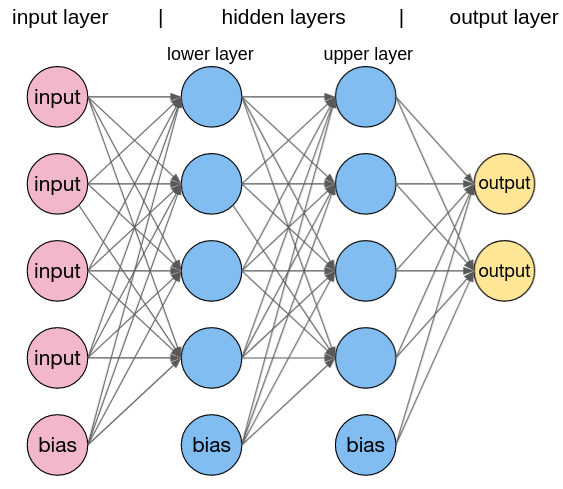
\includegraphics[width=\linewidth]{images/mlp.png}
      \caption[Multilayer Perceptron]{multilayer perceptron} \label{fig:mlp}
    \end{subfigure}%
    \hspace*{\fill}   % maximizeseparation between the subfigures
  \caption[Overview Perceptron]{Overview Perceptron} \label{fig:NN_Overview}
\end{figure}

Convolutional networks, or \glspl{cnn} \cite{lecun1998GradientbasedLearningApplied}, are a specialized type of neural network.
As their name indicates, they perform convolutions on the data as illustrated in \autoref{fig:cnns}.
Convolution can be defined as "a dot-product operation between a grid-structured set of weights and similar grid-structured inputs drawn from
different spatial localities in the input volume" \cite[p. 316]{aggarwal2018NeuralNetworksDeep}.
In other words, a small grid of numbers called \textit{weights} slides over a larger grid of numbers, which is in the context of deep learning usually an image.
In each position, the numbers in the small grid are multiplied by the corresponding numbers they cover in the large grid, and these results are added together. 
This process is repeated across different areas by sliding the small grid over the large grid repeatedly until the complete large grid was processed.
The weights within the small grid, often referred to as the \textit{kernel}, get adjusted during training of the \gls{cnn} during backpropagation. 
This fine-tunes these weights based on how far off the network's output is from the expected output, enabling the convolutional network to improve its performance over time \cite{aggarwal2018NeuralNetworksDeep, Goodfellow-et-al-2016}.

\glspl{cnn} perform exceptionally well on data with a grid-like topology with strong spatial dependencies such as image or time-series data \cite{aggarwal2018NeuralNetworksDeep, Goodfellow-et-al-2016}.
In a typical convolutional network, a layer starts by performing multiple convolution operations in parallel on the data.
The linear activations that are produced by the convolutions are sent through a non-linear activation function (usually a \gls{relu}).
Lastly, a pooling function is applied to the output of the activation function \cite{aggarwal2018NeuralNetworksDeep}.
A pooling function reduces the spatial size of the created feature maps while retaining their essential features \cite{Goodfellow-et-al-2016, aggarwal2018NeuralNetworksDeep}.
\textcite[p. 335]{Goodfellow-et-al-2016} also describe it as a type of "summary statistic of the nearby outputs".
Pooling allows the features extracted by the \gls{cnn} to be less sensitive to changes in the position of the input data.
This property is known as translation invariance and is one of the reasons why \glspl{cnn} perform so well with data formats that have local spatial dependencies \cite{Goodfellow-et-al-2016, aggarwal2018NeuralNetworksDeep}.
Another way to reduce the dimensionality is to increase the convolution stride.
A stride refers to the step size or the number of pixels by which the filter, also known as the convolutional kernel, moves across the input feature map during the convolution operation \cite{aggarwal2018NeuralNetworksDeep}.
The effect of using a stride greater than 1 is that it reduces the spatial dimensions of the output feature map. 
Specifically, the height and width of the output are determined by the formula $(L_q - F_q)/S_q + 1$, where $L_q$ is the height (or width) of the input, $F_q$ is the size of the filter, and $S_q$ is the stride in layer $q$ \cite[p. 324]{aggarwal2018NeuralNetworksDeep}.

In feed-forward neural networks, information flows forward through the network from input to output node, hence, there are no internal connections that allow
the output of the model to be fed back into the network as inputs \cite{aggarwal2018NeuralNetworksDeep, Goodfellow-et-al-2016}.
When such connections are added to the network architecture, the resulting models are referred to as \glspl{rnn} \cite{rumelhart1986LearningRepresentationsBackpropagating}.
\Glspl{rnn} are designed to process sequential data, like sentences or time-series data, where the size of the sequence does not have to be fixed.
In \glspl{cnn}, the learned parameters are shared by using the same convolution kernel on each subset of neighbouring input data at each time step (\autoref{fig:rnns}). 
As a result, a succession of output values is produced, each of which is dependent on a few close input values. 
\glspl{rnn} share parameters differently since each output value depends on its predecessors' output. 
This enables parameter sharing via a deep computational graph by allowing the same update algorithm to be applied to all outputs.
When processing a sequence, \eg a sentence, a \gls{rnn} receives one datapoint, \eg a word, at each timestep.
The network itself has a so-called \textit{hidden state} that is kept throughout all timesteps and changes with each timestep.
This, however, means that the output $y_3$ of the input at $x_{t=3}$ depends on the hidden states $h_0$ through $h_3$ and input $x_0$ through $x_3$.
As a result, the computational graph on which the backpropagation is performed on increases as well \cite{aggarwal2018NeuralNetworksDeep}.
A large computation graph introduces new practical issues, such as an increased computation time and during the training, helpful information might not be propagated from output to the end of the model,
due to the vanishing and exploding gradient phenomenon \cite{aggarwal2018NeuralNetworksDeep}.
To address these issues, further improvements to the architecture have been made, such as \glspl{lstm} \cite{hochreiter1997LongShortTermMemory} or \glspl{gru} \cite{cho2014PropertiesNeuralMachine}.

Over time, additional architectural design choices have been discovered that have led to further improvements and solved other issues that emerged during the development of neural networks.
One such design is the ResNet \cite{he2016DeepResidualLearning} which introduced residual connections between layers as depicted in \autoref{fig:resnet} \cite{he2016DeepResidualLearning, aggarwal2018NeuralNetworksDeep}.
The connections, also called skip connections, allow information to be copied over layers and allow the backpropagated gradient information to skip specific layers, if necessary \cite{he2016DeepResidualLearning, aggarwal2018NeuralNetworksDeep}.
This is achieved by adding the output of one layer directly to the output of a later layer, bypassing one or more intermediate layers.
This way, even a very small gradient can flow more easily back through the network during backpropagation of the gradient, alleviating the vanishing gradient problem and enabling better learning capabilities \cite{he2016DeepResidualLearning, aggarwal2018NeuralNetworksDeep}.
The decision of which layers to skip is learned by the model itself during the training through the backpropagation algorithm \cite{he2016DeepResidualLearning, aggarwal2018NeuralNetworksDeep}.

\begin{figure}
    \begin{subfigure}{0.7\textwidth}
      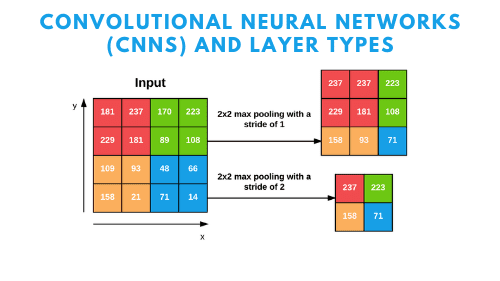
\includegraphics[width=\linewidth]{images/cnns.png}
      \captionsetup{justification=centering}
      \caption{Convolution \\(adapted from \cite{rosebrock2021ConvolutionalNeuralNetworks})} \label{fig:cnns}
    \end{subfigure}%
    \hspace*{\fill}   % maximize separation between the subfigures
    \begin{subfigure}{0.7\textwidth}
      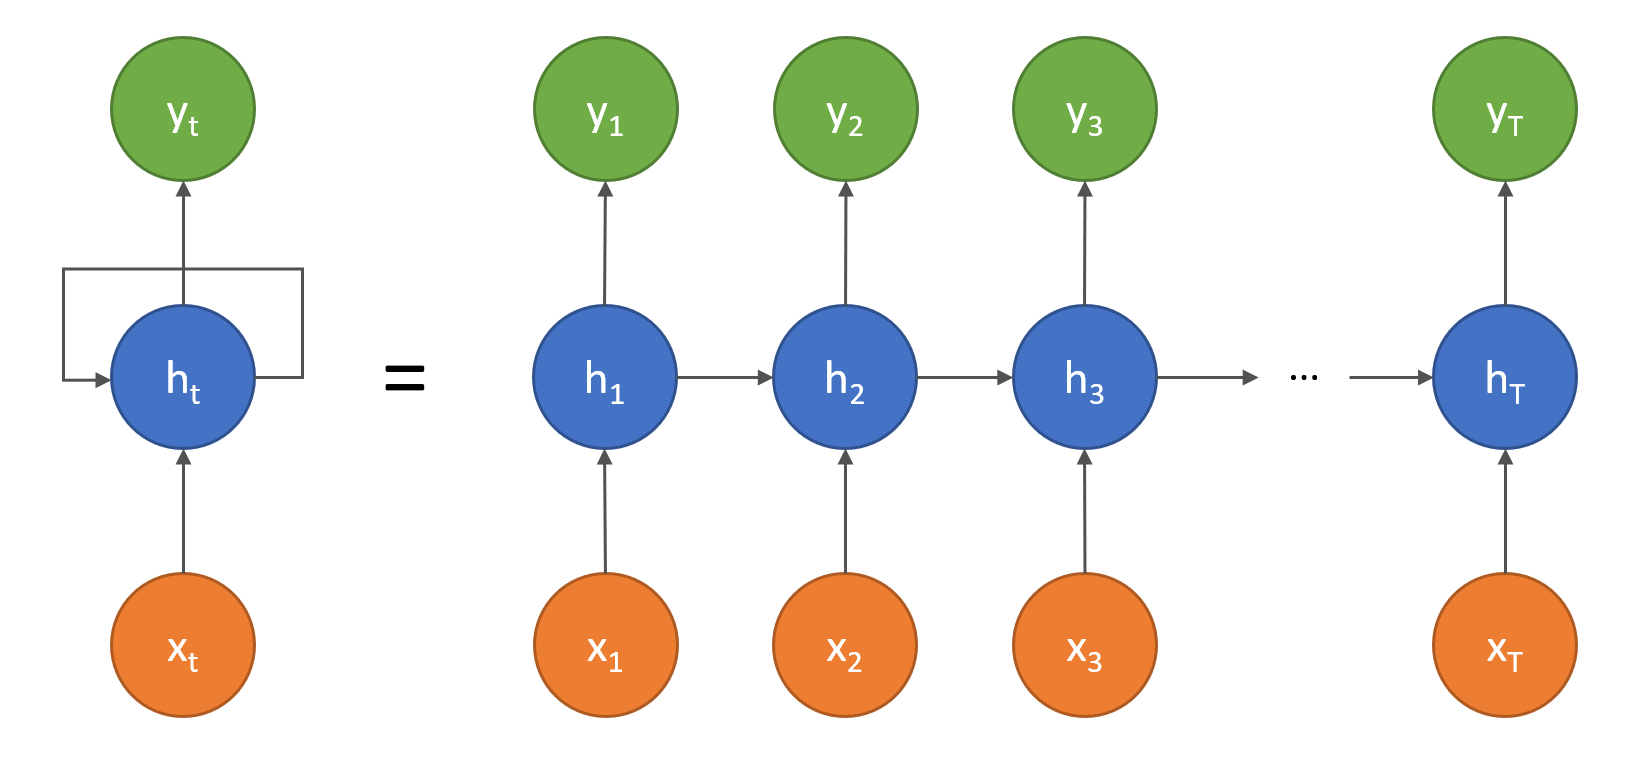
\includegraphics[width=\linewidth]{images/rnns.png}
      \captionsetup{justification=centering}
      \caption{\Gls{rnn} \\(adapted from \cite{radhakrishnan2017IntroductionRecurrentNeural})} \label{fig:rnns}
    \end{subfigure}%
    \hspace*{\fill}   % maximizeseparation between the subfigures
    \begin{subfigure}{0.7\textwidth}
        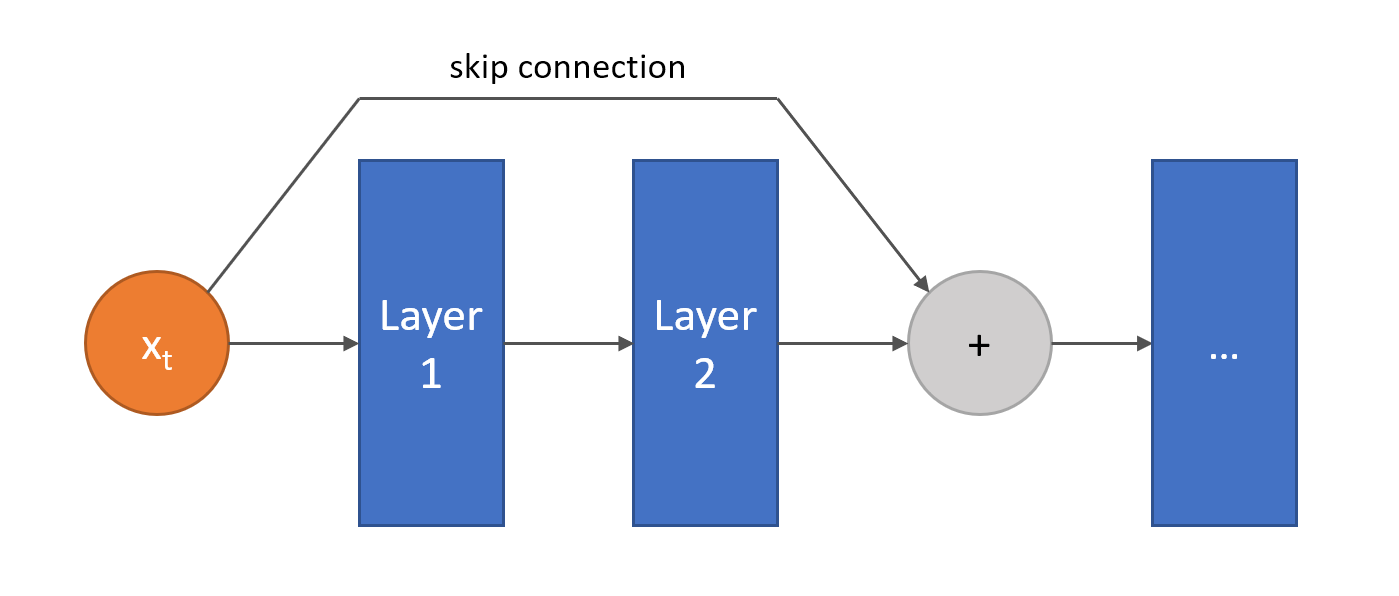
\includegraphics[width=\linewidth]{images/resnet.png}
        \captionsetup{justification=centering}
        \caption{Residual Connection \\(adapted from \cite{hassan2019ResNet3450})} \label{fig:resnet}
      \end{subfigure}%
    \hspace*{\fill}   % maximizeseparation between the subfigures
  \caption[Overview Neural Network Architectures]{Overview Neural Network Architectures} \label{fig:NN_architectures_Overview}
\end{figure}

Lastly, inspired by the human cognitive capabilities to focus on specific parts of an input, attention mechanisms have been introduced \cite{niu2021ReviewAttentionMechanism, aggarwal2018NeuralNetworksDeep}.
The implementation of attention in neural networks tries to address the problem of information overload and is supposed to enable the network to allocate its resources \cite{niu2021ReviewAttentionMechanism}.
Information overload in the context of deep learning typically refers to issues that arise when a model is fed with too much data, that can hinder the model to capture the relevant information.
Issues during training may arise if the input data contains too much noise, that is of no relevance or might cause the model to rather learn to predict the noise, than the actual target.
With this, the model may overfit the training data and perform poorly on the test data. 
An attention mechanism has been successfully applied to various tasks in different domains, such as computer vision or \gls{nlp} \cite{niu2021ReviewAttentionMechanism}.
The architectural realization of attention is realized differently, depending on the task at hand \cite{aggarwal2018NeuralNetworksDeep}.
The attention mechanism in computer vision involves weighting different regions of the image based on their relevance to the task \cite{aggarwal2018NeuralNetworksDeep}. 
This can be achieved through techniques such as spatial attention, channel attention or temporal attention \cite{guo2022AttentionMechanismsComputer}.
In \gls{nlp}, attention mechanisms try to improve to capture the meaning of a sentence \cite{niu2021ReviewAttentionMechanism}. 
For instance, this has been achieved through the introduction of a context vector in an \gls{rnn} encoder-decoder \cite{DBLP:journals/corr/BahdanauCB14} or through self-attention \cite{vaswani2017AttentionAllYou} (see \autoref{ch:preliminaries-transformers} for a detailed explanation of self-attention).

\section{Deep Generative Models}
\label{ch:preliminaries-generativeMlgorithms}

Deep generative models have revolutionized the field of artificial intelligence and machine learning by generating new and original data based on existing patterns and structures. 
Generative models try to learn a joint distribution over all the available variables in a dataset \cite{kingma2019IntroductionVariationalAutoencoders}, which is also called the \textit{generative modeling problem} \cite{goodfellow2020GenerativeAdversarialNetworks}.
Formally, in generative modeling training examples $x$ are drawn from an unknown distribution $p_{data}(x)$ and a generative modeling algorithm is trained to learn a distribution density function $p_{model}(x;\theta)$ that approximates the true probability density function $p_{data}(x)$ as closely as possible \cite[p. 139]{goodfellow2020GenerativeAdversarialNetworks}.
$\theta$ are the models parameters that determine the models output, they are usually learned by searching for best $\theta$ values that result in $p_{model}$ to be as similar to $p_{data}$ as possible \cite[p. 139]{goodfellow2020GenerativeAdversarialNetworks}.

Several powerful generative modeling approaches with different architectures have emerged, each with its strengths and weaknesses. 
This section will explore four of the most popular approaches: \glspl{vae} (\autoref{ch:preliminaries-variationalAutoencoders}), \glspl{gan} (\autoref{ch:preliminaries-generativeAdversarialNetworks}), transformers (\autoref{ch:preliminaries-transformers}), and diffusion models (\autoref{ch:preliminaries-diffusionProbabilisticModels}). 

\subsection{Variational Autoencoders}
\label{ch:preliminaries-variationalAutoencoders} 

In order to understand \glspl{vae} \cite{kingma2013AutoEncodingVariationalBayes}, an introduction to vanilla autoencoders is required.
Autoencoders, firstly introduced in \cite{rumelhart1986LearningInternalRepresentations}, are a neural network architecture designed to generate a copy of the input \cite{Goodfellow-et-al-2016, Bank2020Autoencoders}.
This is done by compressing the original input $x$ into a meaningful representation by constricting the number of nodes in the intermediate hidden layer \cite{aggarwal2018NeuralNetworksDeep, Bank2020Autoencoders}, also called bottleneck.
\autoref{fig:ae} shows that an autoencoder consists of two deep-learning modules, the encoder, and the decoder.
The encoder function (or generative model \cite{kingma2019IntroductionVariationalAutoencoders}), $z=g(x)$ receives an input $x$ and creates a latent representation $z$ (also called "code" \cite{aggarwal2018NeuralNetworksDeep}) with a dimensionality smaller than $x$ \cite{Goodfellow-et-al-2016, Bank2020Autoencoders}.
The decoder (or recognition model \cite{kingma2019IntroductionVariationalAutoencoders}) receives the latent representation $z$ and tries to reconstruct the original input, $r=f(z)$ with the same dimensionality as $x$ \cite{Goodfellow-et-al-2016}.
The reconstruction of the input $x$, designated as $r$, is also commonly referred to as $x'$. 
The objective is to ensure that $x'$ is as similar as possible to the original input $x$.
For the autoencoder to learn and optimize the model's parameters, a loss $L$ is calculated by applying a reconstruction loss function, which measures how close the reconstruction is to its original counterpart \cite{Bank2020Autoencoders, maheshwari2022AutoencoderIssuesChallenges}.
The reconstruction loss depends on the use case, for instance, it could be the Mean-squared error between $x$ and $r$, $L=\sum_{i=1}^{N}(x_i-r_i)^2$ for $N$ features in $x$, \cite{aggarwal2018NeuralNetworksDeep, Goodfellow-et-al-2016}.
Since $z$ is restricted in dimensionality, a simple copying from input to output, \ie $f(g(x))=x$, should not be possible, and the encoder should learn to create an approximation of $x$ with its most essential features \cite{aggarwal2018NeuralNetworksDeep}.
Therefore, autoencoders are a dimensionality reduction technique.
The latent representation of a complete linear autoencoder without any non-linear operations achieves the same representation as a \gls{pca} \cite{plaut2018PrincipalSubspacesPrincipal, Bank2020Autoencoders}.
Further variations of autoencoders have emerged.
Deep autoencoders expand the neural network from one hidden layer to multiple layers with non-linear activation functions, increasing the representation power \cite{aggarwal2018NeuralNetworksDeep}.
Other variants include denoising autoencoders, convolutional autoencoders, or sparse autoencoders \cite{maheshwari2022AutoencoderIssuesChallenges, Goodfellow-et-al-2016}.
However, vanilla autoencoders lack regularity in the latent space which means they struggle with interpolation for datapoints that have not been present in the input sequence \cite{razghandi2022VariationalAutoencoderGenerativea}.




\glspl{vae} increase the reconstruction robustness by letting the decoder sample from continuous distributions \cite{kingma2013AutoEncodingVariationalBayes}.
% \glspl{vae} are, as the name suggests, making use of stochastic variational inference, where the goal is to approximate complex distributions (like the posterior) by simpler ones (like the Gaussian distribution in this case), enabling efficient computation and handling of uncertainty.
This is achieved by introducing the \gls{kl} divergence (see \autoref{eqn:kl-divergence}) to ensure that the latent space representation follows a standard Gaussian distribution (zero mean and unit variance) \cite{razghandi2022VariationalAutoencoderGenerativea, aggarwal2018NeuralNetworksDeep}.
Instead of the encoder mapping the input into a fixed vector $z$, it is mapped into a distribution by generating two vectors representing the mean $\mu$ and standard deviation $\sigma$ of the distribution (see \autoref{fig:vae}) \cite{razghandi2022VariationalAutoencoderGenerativea, aggarwal2018NeuralNetworksDeep}.
Constraining the hidden representation $z$ to a Gaussian distribution allows the decoder to generate new data by simply feeding samples from the standard normal distribution \cite{aggarwal2018NeuralNetworksDeep}.
However, if every object is generated from the same distribution, distinguishing between different objects or reconstructing them from a given input would be impossible.
Thus, the distribution of the encoded information $z$, conditioned on a specific input $x$, would differ from the standard normal distribution \cite{aggarwal2018NeuralNetworksDeep}. %p. 207
Hence, the constraint that the hidden representation $z$ follows a standard normal distribution would not be achieved across the encoded distribution from a single object but rather for the entire dataset \cite{aggarwal2018NeuralNetworksDeep}.
The encoder is represented as $q(z|x)$, creating the conditional distribution from which the latent vector is sampled $z\sim q(z|x)$ \cite{kingma2013AutoEncodingVariationalBayes}.
However, this stochastic sampling process makes computations non-differentiable.
In other words, the backpropagation of the gradient is not possible and our neural networks weights cannot be updated \cite{aggarwal2018NeuralNetworksDeep}.
To address this issue, a "reparameterization trick (\autoref{eqn:reparameterization}) was introduced \cite[p. 4]{kingma2013AutoEncodingVariationalBayes}.
Since $z$ is normally distributed ($z\sim N(\mu,\sigma^2)$) it can be rewritten as $z=\mu+\sigma\epsilon$ with $\epsilon$ used as an auxiliary noise variable $\epsilon \sim N(0,1)$ sampled from the standard normal distribution \cite{kingma2013AutoEncodingVariationalBayes}.

\begin{equation}
  \label{eqn:reparameterization}
  N(\mu,\sigma^2) =\mu+\sigma\epsilon
\end{equation}


This transformation moves the stochastic sampling process to the fixed $\epsilon$ variable. 
It allows $\mu$ and $\sigma$ to be differentiable variables, which enables the gradient to flow and the neural network to learn \cite{kingma2013AutoEncodingVariationalBayes}.
In order for the model to learn that $z$ should be close to a normal distribution, a regularization loss is introduced using the \gls{kl}-divergence.
The \gls{kl}-divergence is defined as:

\begin{equation}
    \label{eqn:kl-divergence}
    KL(p\parallel q) = \sum_{i}^{N}p_i\cdot log(\frac{p_i}{q_i})
\end{equation}

with distributions $p$ and $q$:

\begin{equation}
    \label{eqn:regularization_loss}
    L_{regularization} = KL(q(z|x) \parallel p(z))
\end{equation}

The \gls{kl}-divergence measures how diverged two probability distributions are from one another.
With $p(z)$ as a prior defined standard Gaussian distribution, minimizing this function means optimizing the encoders ($q(z|x)$) parameters of $\mu$ and $\sigma$ towards resembling the distributions it is compared to.

Additionally, a reconstruction loss is computed based on the negative log-likelihood that measures the error between the input and output:
% This reconstruction loss is minimized:
\begin{equation}
    \label{eqn:reconstruction_loss}
    L_{reconstruction} =-\mathbb{E}_{q(z|x)}[logp(x|z)]
\end{equation}
with $E_{q(z|x)}$ denoting the expectation with respect to the encoder distribution.

Hence, the final loss function that is minimized during the training of the \gls{vae} is the combination both loss functions\footnote{The loss components in the original work \cite{kingma2013AutoEncodingVariationalBayes} are formulated as a maximization objective. In practice, a loss that can be minimized during training is required. Hence, we convert the maximization objective to a minimization objective by multiplying it with -1}:

\begin{equation}
    \label{eqn:vae_loss}
    L_{vae} =\mathbb{E}_{q(z|x)}[logp(x|z)]-KL(q(z|x) \parallel p(z))
\end{equation}


\begin{figure}[H]
  \centering
  \begin{subfigure}{0.8\textwidth}
    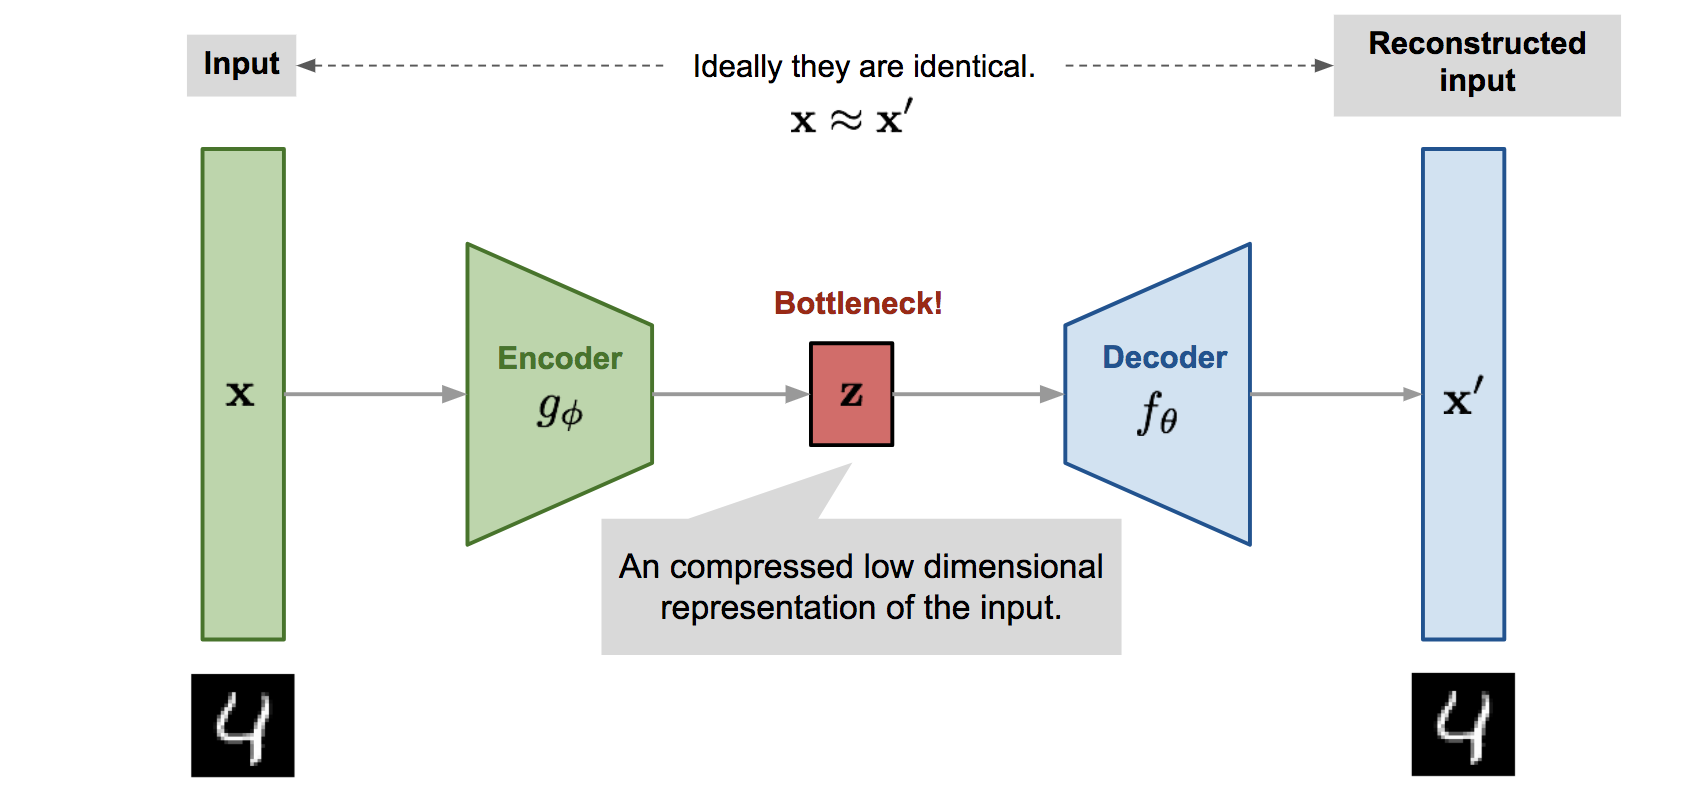
\includegraphics[width=\linewidth]{images/ae.png}
    \caption{Autoencoder} \label{fig:ae}
  \end{subfigure}
  \vspace{\baselineskip}   % separation between the subfigures
  \begin{subfigure}{0.8\textwidth}
    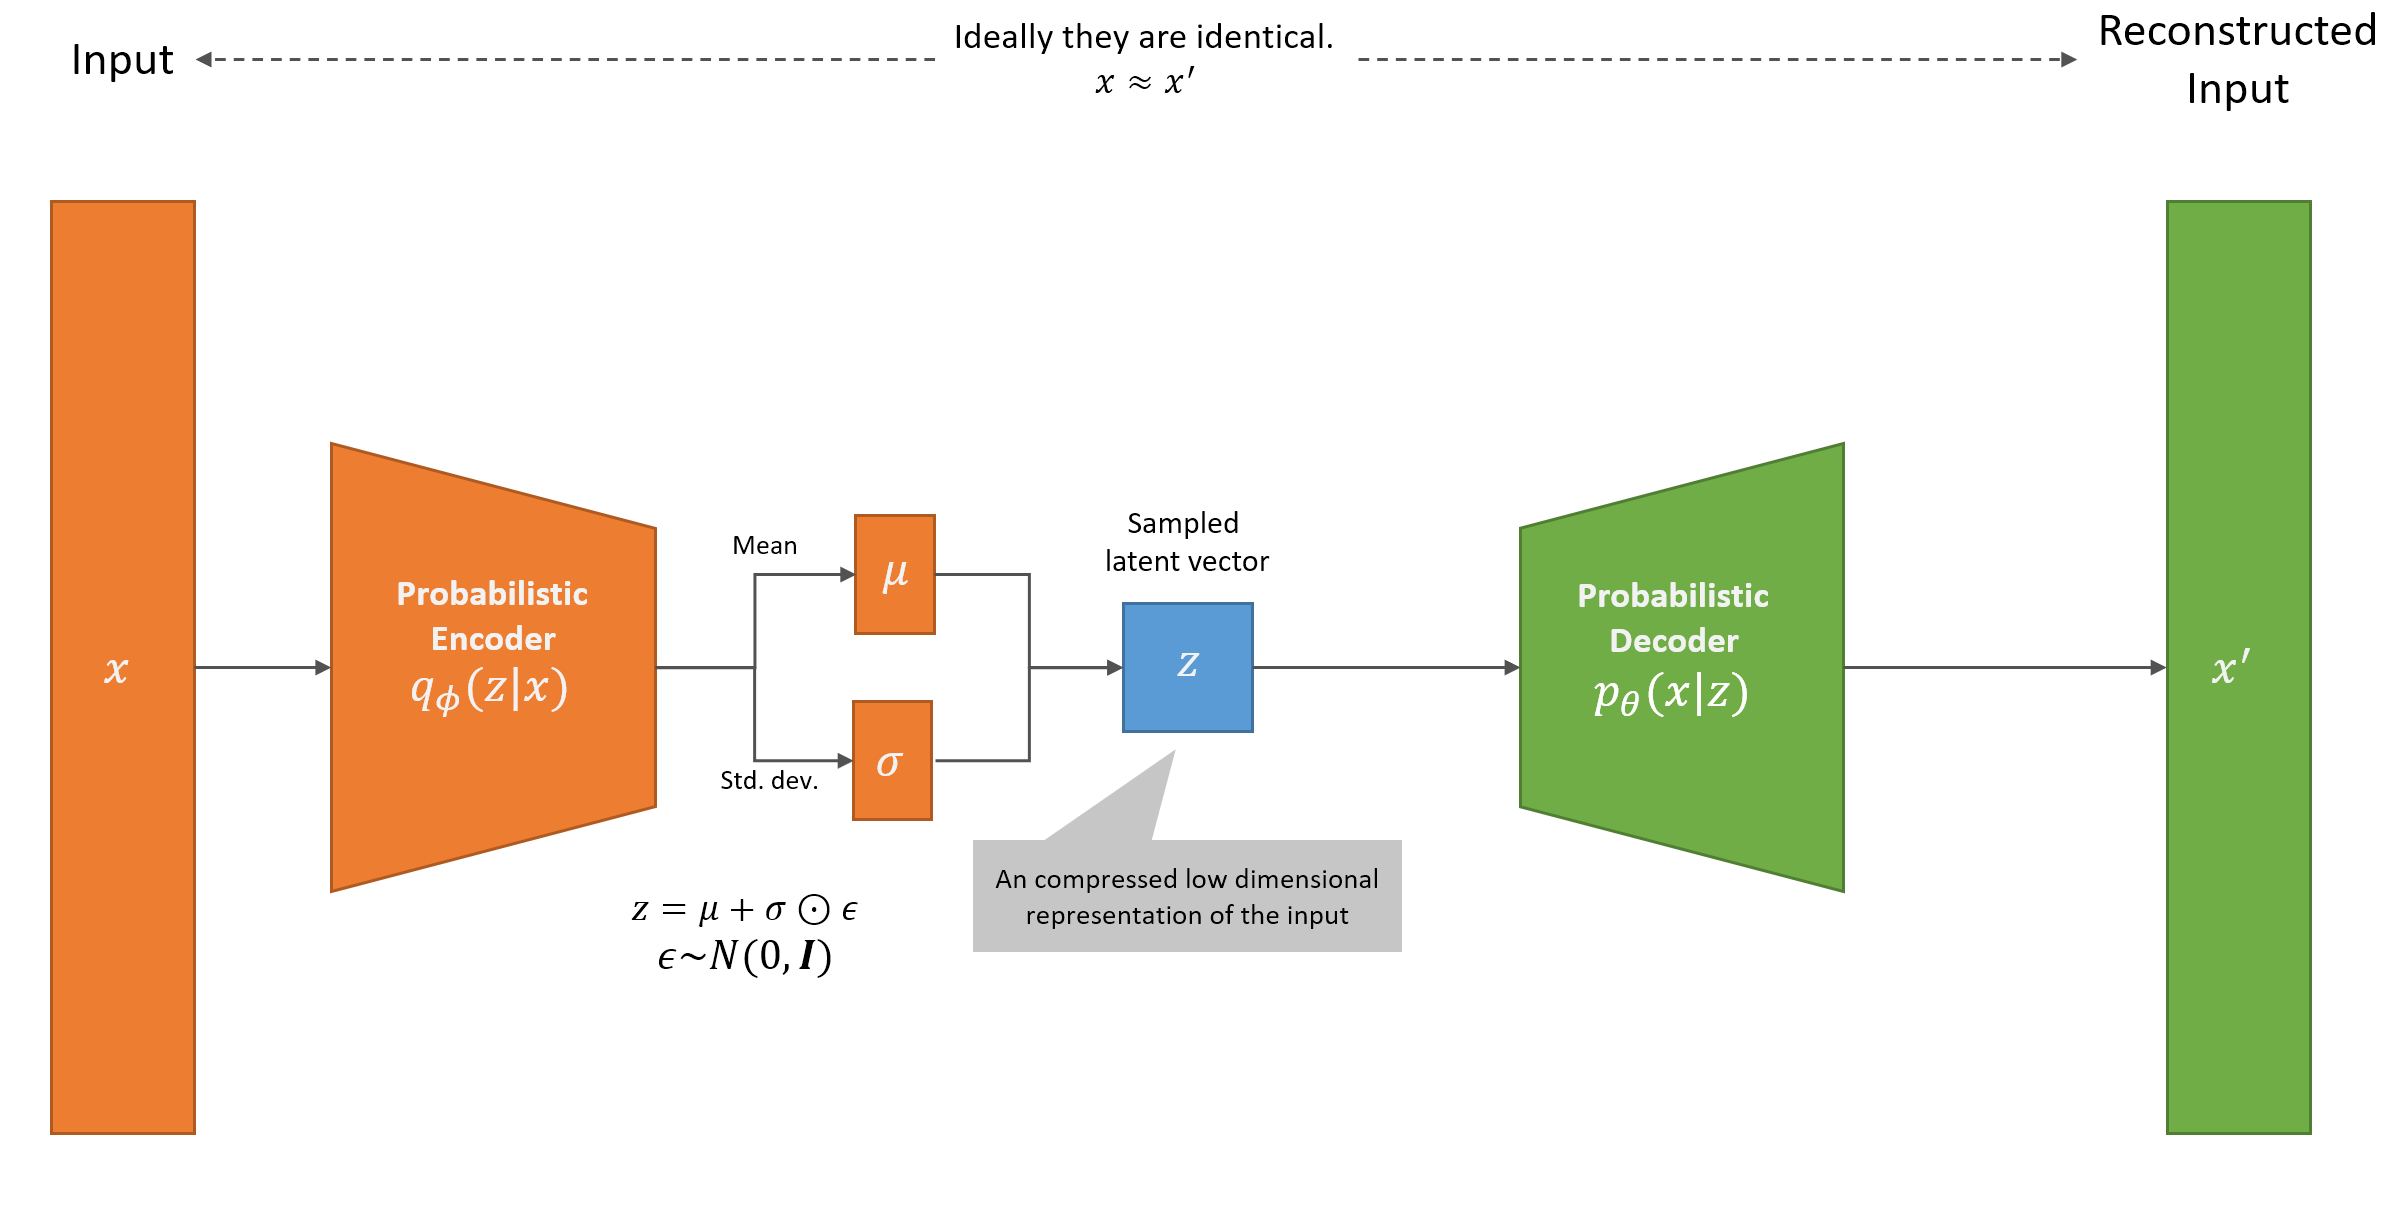
\includegraphics[width=\linewidth]{images/vae.png}
    \caption{Variational Autoencoder} \label{fig:vae}
  \end{subfigure}
\captionsetup{justification=centering}
\caption[Autoencoders]{Architecture of Autoencoder and Variational Autoencoder (adapted from \cite{weng2018AutoencoderBetaVAE})} \label{fig:vae_overview}
\end{figure}



\subsection{Generative Adversarial Networks}
\label{ch:preliminaries-generativeAdversarialNetworks}

\Glspl{gan} \cite{NIPS2014_5ca3e9b1} have been introduced in 2014 as a new architecture to address the generative modeling problem.
The architecture of \glspl{gan} is based on game theory where two models compete in a zero-sum min-max game \cite{NIPS2014_5ca3e9b1, zhao2022CTABGANEnhancingTabular}.
A zero-sum min-max game, in the \glspl{gan}, refers to the adversarial interaction between two models - the generator and the discriminator - where one model's gain (minimizing its loss) corresponds to the other model's loss (maximizing its loss), such that the total sum of their gains and losses is always zero.
While the generator is tasked to generate realistic-looking data points, its adversary, the discriminator is tasked to discriminate whether a given datapoint is a real datapoint or a fake datapoint produced by the generator.
The generator function $G(z;\theta_G)$ with learnable parameters $\theta_G$ receives as input a vector $z$ and is tasked to transform $z$ into a realistic-looking sample $x$.
An input vector $z$ is drawn from a prior distribution $p(z)$, usually a Gaussian or uniform distribution, and is just an unstructured noise vector.
The fake data sample $x=G(z)$ "is intended to be statistically indistinguishable from the training data" $p_{data}$ \cite[p. 141]{goodfellow2020GenerativeAdversarialNetworks}.
The discriminator function $D(x;\theta_D)$ with learnable parameters $\theta_D$ receives as input samples $x$ that could either stem from $p_{data}$ or from $p_{model}$ generated by the generator.
Like a binary classifier, it tries to predict whether a given sample $x$ is real or fake \cite{NIPS2014_5ca3e9b1}.
The discriminators' output classification is finally used in the backpropagation algorithm to update not only the discriminators parameters $\theta_D$, but also the generators parameters $\theta_G$.
So while the generator tries to produce real-looking fake data samples, the discriminator tries to tell real from fake data samples apart. 
This type of training can be seen as a mentor (discriminator) providing feedback to a student (generator) on the quality of his work \cite{zhao2022CTABGANEnhancingTabular}.
Formally, the objective function $J_D$ for the discriminator that will be maximized if real $x$ are correctly classified to $1$ and fake $x$ are correctly classified to $0$ can be defined as \cite{aggarwal2018NeuralNetworksDeep}:

\begin{equation}
    \label{eqn:discriminator}
    Maximize_DJ_D= \sum_{x\in p_{data}}^{} log [D(x)] + \sum_{x\in p_{model}}^{} log [1-D(x)]
\end{equation}

with the first part of \autoref{eqn:discriminator} handling the real data samples and the second part the synthetic data samples.
Hence, the discriminator tries to maximize correctly predicting real and fake samples as real and fake, respectively.

The generator, on the other hand, tries to fool the discriminator.
Therefore, the generator tries to minimize the likelihood that the generated fake samples are flagged as fake.
Its objective function $J_G$ is defined as \cite{aggarwal2018NeuralNetworksDeep}:
\begin{equation}
    \label{eqn:generator}
    Minimize_GJ_G= \sum_{x\in p_{model}}^{} log [1-D(x)] = \sum_{x\in p_z}^{} log [1-D(G(z))]
\end{equation}

Ultimately, the generator and the discriminator are playing a two-player minimax game with the following value function:

\begin{equation}
    \label{eqn:minimax}
    \min_G\max_DV(D,G)=\mathbb{E}_{x\sim p_{data}(x)} [log D(x)] + \mathbb{E}_{z\sim p_z(z)}[log( 1-D(G(Z)))]
\end{equation}

\autoref{eqn:minimax} is used to formulate the loss functions that are used in training.
However, \cite{NIPS2014_5ca3e9b1} notes that in practice, \autoref{eqn:minimax} "may not provide sufficient gradient [for the generator] to learn well" \cite[p. 3]{NIPS2014_5ca3e9b1}.
This seems to be caused by the fact that the discriminator is able to reject the early samples from the generator with high confidence, which results in poor learning capabilities \cite{NIPS2014_5ca3e9b1}.
The proposed solution for this is to change the objective function for the generator from the minimization function \autoref{eqn:generator} to a maximization of $logD(G(z))$.
Thus, instead of minimizing the discriminator being correct, the new objective is to maximize the discriminator being wrong \cite{NIPS2014_5ca3e9b1}. 
\textcite[p. 3]{NIPS2014_5ca3e9b1} observes, that this change "provides much stronger gradients early in learning" and therefore allows for an overall better model learning.
The two loss functions $L_G$ and $L_D$ that are minimized during training of the generator and discriminator, respectively, are defined as:

\begin{equation}
  \begin{align}
  \label{eqn:gan-loss}
  L_D&=logD(x)+log(1-D(G(z)))\\
  L_G&=-log(D(G(z)))
\end{align}
\end{equation}


In practice, the discriminator is trained for $k$ steps for each generator training step \cite{aggarwal2018NeuralNetworksDeep}.
This process is repeated iteratively until a nash equilibrium is reached, at which point the discriminator in unable to tell real and fake samples apart ($p_{model}\approx p_{data}$) \cite{NIPS2014_5ca3e9b1, aggarwal2018NeuralNetworksDeep}.

\subsection{Transformers}
\label{ch:preliminaries-transformers}

In 2017 \textcite{vaswani2017AttentionAllYou} proposed the \textit{transformer} architecture for sequence modeling tasks.
While in this domain \gls{rnn} based approaches have been established state-of-the-art techniques, the newly proposed \textit{transformer} architecture can be trained in a parallel manner,
overcoming the central issue of \gls{rnn}-based models, their high computational demand.
\textit{Transformers} have been successfully adapted in multiple domains, such as \gls{nlp} \cite{gillioz2020OverviewTransformerbasedModels}, computer vision \cite{khan2022TransformersVisionSurvey}, audio processing \cite{gong2022SSASTSelfSupervisedAudio} or 
tabular data \cite{huang2020TabTransformerTabularData} and show properties of a universal computation engine \cite{lu2021PretrainedTransformersUniversal, lin2022SurveyTransformers}.
This is achieved through the combination of several mechanisms, namely, self-attention, multi-head attention, embeddings, and positional encoding \cite{vaswani2017AttentionAllYou}.

The transformer model follows an encoder-decoder structure (see \autoref{fig:transformer}).
The encoder maps an input sequence to an abstract continuous representation that encapsulates all the learned information from the input.
The decoder, in turn, utilizes this representation to generate outputs while also incorporating the previously produced output \cite{vaswani2017AttentionAllYou}.

The first step in the transformer architecture is the transformation of the raw input through an embedding layer (see \autoref{sec:dataTransformation}).
This embedding allows the transformation of input tokens into vectors of dimension $d_{model}$ \cite{vaswani2017AttentionAllYou}.
While the encoder produces embeddings just based on the input sequence, the decoder operates in an autoregressive manner, generating embeddings not only from the encoded output it receives from the encoder, but also considering its own previously produced outputs in the sequence generation process \cite{vaswani2017AttentionAllYou}.
Embeddings of encoder and decoder are combined with so-called positional encodings \cite{vaswani2017AttentionAllYou, lin2022SurveyTransformers}.
Positional encodings have the same dimensionality as the embeddings and carry information about the positions of the tokens in the overall sequence.
\cite{vaswani2017AttentionAllYou} makes use of a $sin$ and $cos$ function to compute this vector.
The sum of the positional encoding vector and the embeddings forms the new input to the encoder or decoder \cite{vaswani2017AttentionAllYou}.

The encoder and decoder consist of multiple blocks, named encoder-blocks and decoder-blocks, respectively.
Each encoder block is based on a multi-head self-attention module, followed by a position-wise feed-forward network.
Residual connections are employed around the two sublayers, followed by a layer normalization, to facilitate building a deeper network \cite{vaswani2017AttentionAllYou, lin2022SurveyTransformers}.

A decoder block is similar to the encoder block; however, an additional multi-head attention module is added at the beginning in front of the other two-sub layers.
Additionally, the self-attention modules in the decoder are adapted in such a way that positions are not able to attend subsequent positions (referred to as "masking" \cite[p. 3]{vaswani2017AttentionAllYou}).
This ensures that predictions for a position can only depend on known outputs \cite{vaswani2017AttentionAllYou, lin2022SurveyTransformers}.

Self-attention allows the model to associate individual words in the input with other words in the input.
This attention mechanism is realized using a scaled Dot-Product on query, key, and value vectors ($Q$, $K$, and $V$ respectively) \cite{vaswani2017AttentionAllYou}.
All three vectors are created by sending the input through different linear layers.
The dot product multiplication of the query and key matrixes creates a score matrix that indicates how much focus an individual word should have on the other words, \ie how much the network should attend to it \cite{vaswani2017AttentionAllYou}.
The created attention matrix is scaled (according to the key dimensionality $d_k$) and multiplied with the value vector to generate the output probabilities.
The multi-head attention refers to the fact that input is split into multiple parts before being processed by different self-attention blocks.
Outputs of the different self-attention blocks are ultimately concatenated back together afterward \cite{vaswani2017AttentionAllYou}.
The attention mechanism can be defined as \cite[p.4]{vaswani2017AttentionAllYou}:

\begin{equation}
  \label{eqn:attention}
  Attention(Q,K,V)=softmax(\frac{QK^T}{\sqrt[]{d_k}})V
\end{equation}

To summarize, the transformer model employs an encoder-decoder structure for sequence modeling tasks. 
The encoder receives an input sequence and transforms it into an abstract continuous representation via an embedding layer, which includes positional encodings. 
This encoded input, containing the attention information from the input, is passed to the decoder. 
The decoder operates in an autoregressive manner, incorporating both the encoded input and a sequence of previously generated outputs in its process. 
The decoder subsequently generates output tokens until it produces an ending token.
Both the encoder and decoder utilize self-attention mechanisms, allowing for context-dependent concentration on different parts of the input sequence.


\begin{figure}
  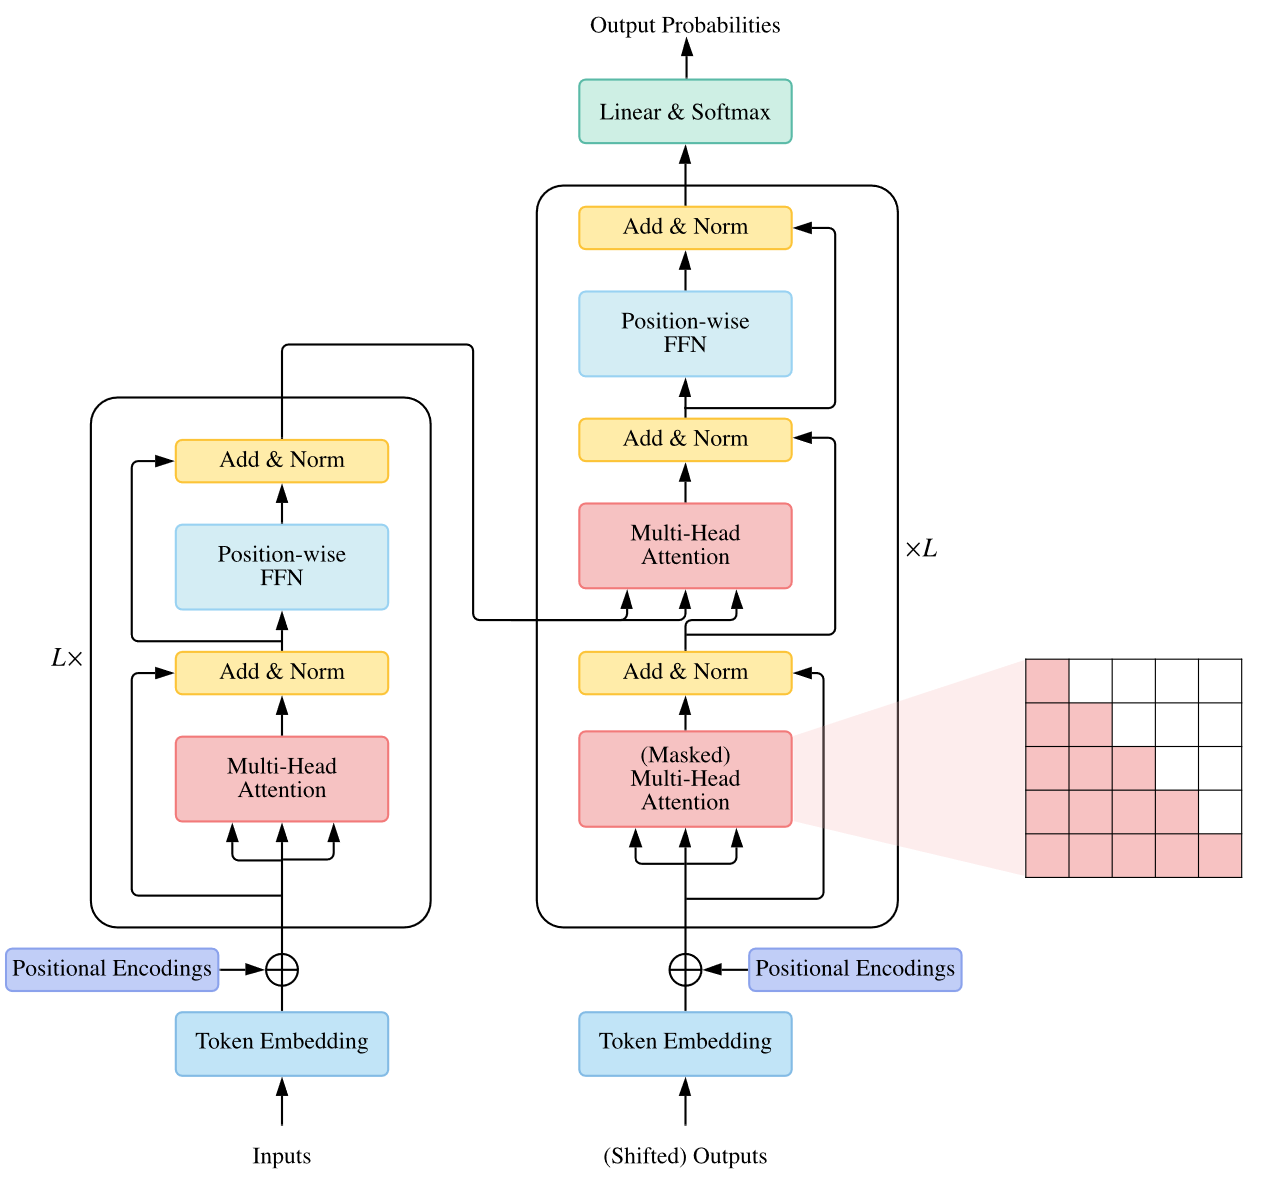
\includegraphics[width=0.8\linewidth]{images/transformer.png}
\caption[Transformers]{Transformer Architecture \cite[Figure 1, p. 3]{lin2022SurveyTransformers}} \label{fig:transformer}
\end{figure}


\subsection{Diffusion Probabilistic Models}
\label{ch:preliminaries-diffusionProbabilisticModels}

The \Glspl{ddpm} (from now on referred to as "diffusion model"), firstly introduced by \textcite{sohl-dickstein2015DeepUnsupervisedLearning}, is a generative modeling approach inspired by non-equilibrium statistical physics \cite{sohl-dickstein2015DeepUnsupervisedLearning}.
\textcite{ho2020DenoisingDiffusionProbabilistic} in their work, how diffusion models can successfully generate high-quality synthetic images.
This section will provide an explanatory introduction to the diffusion model concept, drawing heavily on the foundational work of \cite{ho2020DenoisingDiffusionProbabilistic}.
Although several other researchers have made notable advancements to diffusion probabilistic models, the work presented in \cite{sohl-dickstein2015DeepUnsupervisedLearning, ho2020DenoisingDiffusionProbabilistic} 
serves as the cornerstone upon which all subsequent improvements have been built.
Improvements and alternations made to \cite{ho2020DenoisingDiffusionProbabilistic} will be discussed in detail in \autoref{ch:relatedWork-diffusionModels}.

On a high level, the whole diffusion concept can be summarized as follows:

\begin{quotation}
  "The essential idea, (...) is to systematically and slowly destroy structure in a data distribution through an iterative forward diffusion process. 
  We then learn a reverse diffusion process that restores structure in data, yielding a highly flexible and tractable generative model of the data." \cite[p. 1]{sohl-dickstein2015DeepUnsupervisedLearning}
\end{quotation}

Formally, \cite{ho2020DenoisingDiffusionProbabilistic} defines diffusion models as a class of \glspl{lvm} of the form $p_\theta(x_0):= \int_{}^{}p_\theta(x_{0:T})dx_{1:T}$,
with $x_1, ..., x_T$ as latents of the same dimensionality as samples from the data distribution $x_0 \sim q(x_0)$.
Diffusion models consist of a forward process and a reverse process.
During the forward process, an initial data point $x_0$ is obtained from the data distribution $q(x_0)$.
In the forward process (also called diffusion process), a fixed \gls{mc} gradually adds noise to the data.
$T$ defines the number of noising steps and $x_1,...,x_T$ denotes the latent variables, \ie the noised versions of the original data, with $x_T$ being the fully noised version of the data \cite{ho2020DenoisingDiffusionProbabilistic}.
The amount of added (Gaussian) noise in each timestep varies depending on the current timestep, which is controlled by a variance schedule $\beta_1, ..., \beta_T \in (0,1)$ \cite{ho2020DenoisingDiffusionProbabilistic}.
The forward process is defined as:

\begin{equation}
  \label{eqn:forwards_1}
  \begin{align*}
    q(x_{1:T} | x_0) := \prod_{t=1}^T q(x_t | x_{t-1}), \quad
    q(x_t | x_{t-1}) := \mathcal{N}(x_t; \sqrt{1 - \beta_t} x_{t-1}, \beta_t I)
  \end{align*}
\end{equation}

For the variance schedule it holds that if $\beta_1 < \beta_2 < ... < \beta_T$ for $t\rightarrow\infty$, the final latent $x_t$ is isotropic Gaussian noise, \ie, $x_t \sim \mathcal{N}(0, \textbf{I})$, with identity matrix $\textbf{I}$ \cite{zbinden2022ImplementingExperimentingDiffusion}.
$\beta$ increases linearly in the original \gls{ddpm} approach \cite{ho2020DenoisingDiffusionProbabilistic} but was later improved to follow a cosine schedule \cite{nichol2021ImprovedDenoisingDiffusion}, improving the overall quality of the model.

\autoref{eqn:forwards_1} \cite{ho2020DenoisingDiffusionProbabilistic} shows how iteratively one noising step can be applied to get from $x_{t-1}$ to $x_t$ with $q(x_t | x_{t-1})$.
Through the use of a reparameterization (see \autoref{eqn:reparameterization}) and defining $\alpha := 1-\beta_t$ and $\overline{\alpha_t}:=\prod_{s=1}^{t}a_s$, 
the forward diffusion process from an unnoised input $x_0$ to a noised version at $t$ can be expressed as follows:

\begin{equation}
  \label{eqn:forwards_2}
  \begin{align*}
    q(x_t | x_0) \quad & := \mathcal{N}(x_t; \sqrt{\bar{\alpha}_t} x_0, (1 - \bar{\alpha}_t) \textbf{I})\\
    %  x_t &= \sqrt{\bar{\alpha}_t} x_0 + \sqrt{1 - \bar{\alpha}_t} \epsilon \textrm{, with } \epsilon\sim\mathcal{N}(0, \textbf{I})
  \end{align*}
\end{equation}

\autoref{eqn:forwards_2} \cite{ho2020DenoisingDiffusionProbabilistic} allows computing the forward noising from $x_0$ to any timestep $t$ within one computation step instead of iteratively applying noise over and over again.

During the reverse process, the goal is to learn the reverse distribution from noised data $x_t$ to slightly less noised data $x_{t-1}$, $q(x_{t-1}|x_t)$.
With bayes-theorem we can see that $q(x_{t-1}|x_t) = \frac{p(x_{t-1},x_t)}{p(x_t)}$, which means $q(x_{t-1}|x_t)$ depends on the marginal distribution of $x_t$, denoted as $p(x_t)$.
To calculate the marginal probability distribution $p(x_t)$ integration over all possible realizations of $x_{t-1}$ would be necessary, which would be computationally intractable \cite{capel2022MasterThesisDenoising}.
As a result, $q(x_{t-1}|x_t)$ is approximated by a neural network with learnable parameters $\theta$ that learns the joint distribution $p_{\theta}(x_{0:T})$.
$p_{\theta}(x_{0:T})$ is a \gls{mc}, defined in \autoref{eqn:reverse_1}, with the transitions defined in \autoref{eqn:reverse_2} \cite{capel2022MasterThesisDenoising, ho2020DenoisingDiffusionProbabilistic}.

\begin{equation}
  \label{eqn:reverse_1}
  \begin{align*}
    p_{\theta}(x_{0:T}) := p(x_T) \prod_{t=1}^T p_{\theta}(x_{t-1} | x_t),
  \end{align*}
\end{equation}

\begin{equation}
  \label{eqn:reverse_2}
  \begin{align*}
    p_{\theta}(x_{t-1}|x_t) := \mathcal{N}(x_{t-1}; \mu_{\theta}(x_t, t), \Sigma_{\theta}(x_t, t))
  \end{align*}
\end{equation}
    
While the mean $\mu_{\theta}(x_t, t)$ is learned by the neural network, the variance $\Sigma_{\theta}(x_t, t)$ stayed fixed in the initial work by \cite{ho2020DenoisingDiffusionProbabilistic} 
but was later in \textcite{nichol2021ImprovedDenoisingDiffusion} work a learnable parameter as well \cite{zbinden2022ImplementingExperimentingDiffusion}.

Like in \glspl{vae} (\autoref{ch:preliminaries-variationalAutoencoders}), the model is trained by minimizing its negative log-likelihood (= maximizing the log-likelihood) $-log(p_\theta(x_0))$.
$p_\theta(x_0)$ depends on all timesteps before $x_0$ and is, therefore, not tractable in practice \cite{zbinden2022ImplementingExperimentingDiffusion}.
As a solution, the variational lower bound on the negative log-likelihood can be computed \autoref{eqn:vlb}: %(ELBO)

\begin{equation}
  \label{eqn:vlb}
  \begin{align*}
    -log(p_\theta(x_0)) \leq -log(p_\theta(x_0)) + KL(q(x_{1:T}|x_0) \parallel p_\theta(x_{1:T}|x_0))
  \end{align*}
\end{equation}

The \gls{kl}-divergence (\autoref{eqn:kl-divergence}) is a non-negative measure of dissimilarity between two probability distributions. 
The right-hand side is reduced by minimizing the \gls{kl}-divergence as the objective function in the given inequality, leading to a smaller or equal left-hand side. 
Consequently, minimizing the \gls{kl}-divergence can only decrease the negative log-likelihood term on the left-hand side of the inequality. 
This implies that the objective function provides a lower bound on the log-likelihood and any improvement in minimizing the \gls{kl}-divergence will ultimately lead to an enhancement in this lower bound.
Rewriting $KL(q(x_{1:T}|x_0) \parallel p_\theta(x_{1:T}|x_0))$ to $log(\frac{q(x_{1:T})|x_0}{p_\theta(x_{1:T}|x_0)})$ and some reformulations (see \autoref{eqn:vlb2_appendix}) using bayes-rule results in \autoref{eqn:vlb2} leads to the following inequation \cite{ho2020DenoisingDiffusionProbabilistic}:

\begin{equation}
  \label{eqn:vlb2}
  \begin{align*}
    -log(p_\theta(x_0)) \leq log(\frac{q(x_{1:T})|x_0)}{p_\theta(x_{0:T})})
  \end{align*}
\end{equation}

\autoref{eqn:vlb2} is the variational lower bound that is minimized during training to optimize $-log(p_\theta(x_0))$.
With additional reformulations (see \autoref{eqn:vlb3_appendix}), the loss function can be derived as \cite{ho2020DenoisingDiffusionProbabilistic}:

\begin{equation}
  \label{eqn:vlb3}
  \begin{align*}
   \mathbb{E}\biggl[\underbrace{D_{KL}(q(x_{T}|x_0) \parallel p(x_T))}_{L_T} + \sum_{t>1}^{} \underbrace{  D_{KL}(q(x_{t-1}|x_t,x_0) \parallel p_\theta(x_{t-1}|x_t)) }_{L_{t-1}}  \underbrace{ -log p_\theta(x_0|x_1) }_{L_{0}}\biggr]
  \end{align*}
\end{equation}

$L_T$ consists of $q(x_{T}|x_0)$ and is a noising forward process that has no learnable parameters and $p(x_T)$ is Gaussian distributed noise.
If the forward process correctly destroys the data, $q(x_{T}|x_0)$ will converge to a standard Gaussian distribution as well and one can be confident that $L_T$ will be close to $0$.
Thus, $L_T$ will be neglected.

To $L_{0}$ can also be referred to as a "reconstruction term" \cite[p. 10]{luo2022UnderstandingDiffusionModels}.
\textcite{ho2020DenoisingDiffusionProbabilistic} initially use an independent discrete decoder to determine $L_{0}$, derived from $\mathcal{N}(x_0;\mu_0(x_1,1)\sigma^2_1,\textbf{I})$.
However, ultimately the authors decide to remove the term in favor of a simpler loss term, which leads to a simpler implementation and better quality \cite{ho2020DenoisingDiffusionProbabilistic}.

Inside $L_{t-1}$, one compares the target denoising step $q(x_{t-1}|x_t,x_0)$ that is also conditioned on the input $x_0$ with the approximated denoising step $p_\theta(x_{t-1}|x_t)$. %%%
Both terms have a closed-form solution (meaning they can be computed within a finite amount of standard computations) thanks to the conditioning on $x_0$ \cite{ho2020DenoisingDiffusionProbabilistic}:

\begin{equation}
  \label{eqn:lt-1_1}
  p_\theta(x_{t-1}|x_t)= \mathcal{N}(x_{t-1};\mu_\theta(x_t,t), \beta\textbf{I})
\end{equation}

\begin{equation}
  \label{eqn:lt-1_2}
q(x_{t-1}|x_t,x_0) = \mathcal{N}(x_{t-1};\tilde{\mu_t}(x_t,x_0), \tilde{\beta_t}\textbf{I})
\end{equation}

\autoref{eqn:lt-1_2} can be further simplified, considering that:
\begin{equation}
  \begin{align}
    &\tilde{\mu_t}(x_t, x_0) := \frac{\sqrt{\bar{\alpha}_{t-1}}\beta_t}{1 - \alpha_{\bar{t}}}x_0 +   \frac{\sqrt{\alpha_t}(1-\bar{\alpha}_{t-1})}{1 - \bar{\alpha}_{t}}x_t \quad \textrm{and }
    \tilde{\beta_t}:=\frac{1-\bar{\alpha}_{t-1}}{1-\bar{\alpha}_t}\beta_t \nonumber\\
  \end{align}
\end{equation}
    
\begin{equation}
  \begin{align}
    &x_t = \sqrt{\bar{\alpha}_{t}}x_0+\sqrt[]{1-\bar{\alpha}_t}\epsilon \quad\textrm{and }
    x_0 = \frac{1}{\sqrt{\bar{\alpha}_t}}(x_t-\sqrt[]{1-\bar{\alpha}_t}\epsilon) \nonumber\\
  \end{align}
\end{equation}

with $\beta$ being fixed by \cite{ho2020DenoisingDiffusionProbabilistic} and the mean $\tilde{\mu_t}$ is being further simplified to \autoref{eqn:lt-1_3} \cite{ho2020DenoisingDiffusionProbabilistic}:

\begin{equation}
  \begin{align}
    \label{eqn:lt-1_3}
    \tilde{\mu_t}(x_t, x_0) = \frac{1}{\sqrt{\bar{\alpha}_t}}(x_t - \frac{\beta_t}{\sqrt[]{1-\bar{\alpha}_t}}\epsilon)
  \end{align}
\end{equation}

which is just scaled random noise that is subtracted from $x_t$, the fully noised data.

Hence, the \gls{kl}-divergence in $L_{t-1}$ in \autoref{eqn:vlb2} ultimately measures the difference between the actual noise that was added ($\tilde{\mu_t}$ in \autoref{eqn:lt-1_3}) and the predicted noise from the neural network ($\mu_\theta$ in \autoref{eqn:lt-1_1}).
\textcite{ho2020DenoisingDiffusionProbabilistic} proposes the \gls{mse} between $\tilde{\mu_t}$ and $\mu_\theta$ as a loss function:

\begin{equation}
  \begin{align}
    \label{eqn:mse_loss}
    L_{t-1} = \mathbb{E}_q \left[ \frac{1}{2\sigma_t^2} \left\Vert \tilde{\mu}_t(x_t, x_0) - \mu_\theta(x_t, t) \right\Vert^2 \right] + C
  \end{align}
\end{equation}

The constant $C$ will be removed during training, as it does not depend on $\theta$ \cite{ho2020DenoisingDiffusionProbabilistic}.
By applying the same reparameterization that was done in \glspl{vae} (see \autoref{eqn:reparameterization}) to $\mu_\theta$, it can be reformulated in the following way:

\begin{equation}
  \begin{align}
    \label{eqn:mse_loss_2}
    \mu_\theta(x_t,t)= \frac{1}{\sqrt{\alpha_t}}(x_t - \frac{\beta_t}{\sqrt[]{1-\bar{\alpha}_t}}\epsilon_\theta(x_t,t)) 
  \end{align}
\end{equation}

With the reparameterization of \autoref{eqn:mse_loss_2}, the parametrization of what the model should predict in the reverse process (from $x_t$ to $x_{t-1}$) is moved. 
Instead of predicting the mean and variance of the reverse distribution ($p_\theta(x_{t-1}|x_t)$), \ie directly predicting the less noised data, 
the model predicts the noise $\epsilon$ that makes the difference between $x_{t-1}$ and ${x_t}$.
In other words, instead of predicting the new data directly, the model learns to predict what noise it needs to remove from the data \cite{capel2022MasterThesisDenoising}.
Ultimately, during sampling $x_{t-1}$ can be calculated by:

\begin{equation}
  \begin{align*}
    \label{eqn:xt-1}
    x_{t-1} = \frac{1}{\sqrt{\alpha_t}}\left(x_t - \frac{\beta_t}{\sqrt{1-\bar{\alpha}t}}\epsilon_{\theta}(x_t,t)\right) + \sigma_t z \textrm{,}\quad
    \textrm{with } \beta_t := 1-\alpha_t
  \end{align*}
\end{equation}

Where $z\sim\mathcal{N}(0,\textbf{I})$ is a random component that is added during the reverse process (except for $t=1$) to ensure the generation of diverse samples.

Substituting $\tilde{\mu_t}$ as in \autoref{eqn:lt-1_3} and $\mu_\theta$ as in \autoref{eqn:mse_loss_2} with some further simplification leads to:

\begin{equation}
  \begin{align*}
    \label{eqn:eqn:lt-1_4}
    L_{t-1} &= \mathbb{E}_{x_0,\epsilon} \left[  \frac{\beta^2_t}{2\sigma_t^2 \alpha_t (1-\bar{\alpha}_t)} ||\epsilon - \epsilon_\theta(x_t,t)||^2 \right] \\
    &= \mathbb{E}_{x_0,\epsilon} \left[  \frac{\beta^2_t}{2\sigma_t^2 \alpha_t (1-\bar{\alpha}_t)} ||\epsilon - \epsilon_\theta( \underbrace{\sqrt{\bar{\alpha}_t} x_0 + \sqrt{1-\bar{\alpha}_t}\epsilon}_{x_t}, t)||^2 \right]
  \end{align*}
\end{equation}


Ultimately, \textcite[p. 5]{ho2020DenoisingDiffusionProbabilistic} discovered that simplifying the loss term even further improves not only the sample quality but is also easier to implement.
\autoref{eqn:l_simple} shows the final simplified loss function $L_{simple}$:

\begin{equation}
  \begin{align*}
    \label{eqn:l_simple}
    L_{simple}(\theta) = \mathbb{E}_{t, x_0,\epsilon} \left[ ||\epsilon - \epsilon_\theta( \sqrt{\bar{\alpha}_t} x_0 + \sqrt{1-\bar{\alpha}_t}\epsilon, t)||^2 \right]
  \end{align*}
\end{equation}

\textcite{ho2020DenoisingDiffusionProbabilistic} state that this simplified loss version is a weighted variational bound, which down-weights the loss for small $t$'s, which corresponds to data point with only little added noise.
They further argue that this is actually beneficial for the model since learning small noise is not difficult. 
Therefore the model can focus more on the large $t$'s, where the denoising is more difficult \cite{ho2020DenoisingDiffusionProbabilistic}.

\autoref{alg:training} shows the full training algorithm, which will be realized by firstly randomly sampling a datapoint $x_0 \sim q(x_0)$ from the dataset, a timestep $t\sim Uniform(\{1, ..., T\})$ and some random Gaussian noise $\epsilon \sim \mathcal{N}(0, \textbf{I})$.
Afterward, the gradient step will then be performed according to \autoref{eqn:l_simple} using gradient descent.

\begin{algorithm}[T]
  \caption[Training algorithm]{Training \cite[p. 4]{ho2020DenoisingDiffusionProbabilistic}}
  \label{alg:training}
  \begin{algorithmic}
    \Repeat
    \State $x_0 \sim q(x_0)$
    \State $t\sim Uniform(\{1, ..., T\})$
    \State $\epsilon \sim \mathcal{N}(0, \textbf{I})$
    \State Take gradient descent step on
    \State \hskip1.5em $\nabla_\theta||\epsilon - \epsilon_\theta( \sqrt{\bar{\alpha}_t} x_0 + \sqrt{1-\bar{\alpha}_t}\epsilon, t)||^2$
    \Until converged
  \end{algorithmic}
\end{algorithm}


Sampling, on the other hand, follows \autoref{alg:sampling}, starting with sampling Gaussian noise $x_T$.
The Gaussian noise is then denoised in an iterative manner for $T$ timesteps according to \autoref{eqn:xt-1} until a new, noise-free datapoint $x_0$ is generated.

\begin{algorithm}[H]
\caption[Sampling algorithm]{Sampling algorithm \cite[p. 4]{ho2020DenoisingDiffusionProbabilistic}}
  \label{alg:sampling}
  \begin{algorithmic}
  \State $x_T \sim \mathcal{N}(0, \mathbf{I})$
  \For{$t = T, \dots, 1$}
  \State $z \sim \mathcal{N}(0, \mathbf{I})$ if $t > 0$ else $z = 0$
  \State $x_{t-1} = \frac{1}{\sqrt{\alpha_t}}\left(x_t - \frac{\beta_t}{\sqrt{1-\bar{\alpha}t}}\epsilon_{\theta}(x_t,t)\right) + \sigma_t z$
  \EndFor
  \State \Return $x_0$
  \end{algorithmic}
\end{algorithm}

In summary, \cite{ho2020DenoisingDiffusionProbabilistic} introduced \gls{ddpm} based on the work of \cite{sohl-dickstein2015DeepUnsupervisedLearning}.
Their diffusion model is based on a \gls{mc} and consists of the forward noising and the backward denoising part.
During the forward process, a timestep $t$ is sampled and the raw input data $x_0$ is noised accordingly using \autoref{eqn:forwards_2}.
A function approximator (usually a neural network) with learnable parameters $\theta$ tries to remove the noise by predicting the noise that was added during the forward process.
This difference between the actual noise $\epsilon$ and the predicted noise $\epsilon_{\theta}$ is used as a loss function (\autoref{eqn:l_simple}) to perform gradient descent.
Once the training is finished, and the model converges, new synthetic data can be generated during sampling.
In the sampling process, Gaussian noise can be sampled, and the model progressively denoises the sample for $T$ timesteps until a new, denoised datapoint $x_0$, is generated.


\subsection{Multinomial Diffusion}
\label{ch:multinomial}
The \gls{ddpm} apprach uses a Gaussian diffusion process, designed to operate in continuous space \cite{kotelnikov2022TabDDPMModellingTabular}.
However, many different data types are of categorical nature, where the Gaussian noising process proposed in \autoref{ch:preliminaries-diffusionProbabilisticModels} is not applicable.
As a response, \textcite{hoogeboom2021ArgmaxFlowsMultinomial} introduced multinomial diffusion, "a diffusion model directly defined on categorical variables" \cite[p, 3]{hoogeboom2021ArgmaxFlowsMultinomial}.

\cite{hoogeboom2021ArgmaxFlowsMultinomial} defines the multinomial diffusion process in the following way:

\begin{equation}
  \begin{align*}
    \label{eqn:mul_diff1}
    q(x_{t}|x_{t-1}) = \mathcal{C}(x_t|(1-\beta_t)x_{t-1}+\beta_t/K)
  \end{align*}
\end{equation}


The term $\beta_t$ denotes the likelihood of swapping the current categorical value with a different one. 
Essentially, it is deciding how much random variation, or "noise", is introduced.
This noise is based on a categorical uniform distribution, which means that it considers all available categories equally when picking a random value \cite{hoogeboom2021ArgmaxFlowsMultinomial}.
Furthermore, $\mathcal{C}$ denotes a categorical distribution and $x_t$ is represented in a \gls{oh} encoded categorical vector format with $K$ different classes, $x_t\in\{0,1\}^K$ \cite{hoogeboom2021ArgmaxFlowsMultinomial}.

The noising step from $x_0$ to any noised version $x_t$ can be expressed as:

\begin{equation}
  \begin{align*}
    \label{eqn:mul_diff2}
    q(x_{t}|x_{0}) = \mathcal{C}(x_t|\overline{\alpha}_tx_{0}+(1-\overline{\alpha}_t)/K)
  \end{align*}
\end{equation}

with $\alpha_t = 1-\beta_t$ and $\overline{\alpha}_t = \prod_{\tau=1}^{t}\alpha_\tau$.
Uniform noise is added over the $K$ classes in each timestep.
If $(1-\beta_t)$ is large, the model is likely to retain the previous category from $x_{t-1}$. 
Likewise, if $(1-\beta_t)$ is small, the model will rely more on sampling a random category from a uniform distribution over all categorical values for the variable.

\cite{hoogeboom2021ArgmaxFlowsMultinomial} derives from \autoref{eqn:mul_diff1} and \autoref{eqn:mul_diff2} the categorical posterior:

\begin{equation}
  \begin{gathered}
  \label{eqn:mul_diff3}
  q(x_{t-1}|x_t, x_{0}) = \mathcal{C}(x_{t-1}|\theta_{post}(x_t,x_0)),\textrm{ where } \theta_{post}(x_t,x_0)=\tilde{\theta}/\sum_{k=1}^{K}\tilde{\theta}_k \\
  \textrm{and } \tilde{\theta} = \left[\alpha_tx_{t}+(1-\alpha_t)/K \right] \odot \left[\overline{\alpha}_{t-1}x_{0}+(1-\overline{\alpha}_{t-1})/K \right]
  \end{gathered}
\end{equation}

\cite{hoogeboom2021ArgmaxFlowsMultinomial} argues, that predicting the added noise, as in \cite{ho2020DenoisingDiffusionProbabilistic},
is difficult, and instead the authors predict a probability vector for $\hat{x_0}$ from $x_t$.
The reverse distribution $p_\theta(x_{t-1}|x_t)$ is realized in the form of $q(x_{t-1}|x_t,\hat{x_0})$ where $\hat{x_0}=\mu(x_t, t)$ is predicted by the model and tries to approximate $x_0$ \cite{hoogeboom2021ArgmaxFlowsMultinomial}.
Hence:

\begin{equation}
  \begin{align*}
    \label{eqn:mul_diff4}
    p(x_0|x_1) = \mathcal{C}(x_0|\hat{x}_0) \textrm{ and } p(x_{t-1}|x_t) =  \mathcal{C}(x_{t-1}|\theta_{post}(x_t, \hat{x}_0)) \textrm{ where } \hat{x}_0=\mu(x_t,t)
  \end{align*}
\end{equation}

In other words, determining the categorical value assigned to $x_{t-1}$ (or $x_0$ in the last step) is based on the predicted probabilities $\hat{x}_0$ produced by the model.


The loss function in terms of \gls{kl}-divergence (\autoref{eqn:vlb3}) can be computed with \autoref{eqn:mul_diff3} and \autoref{eqn:mul_diff4}:

\begin{equation}
  \begin{align*}
    \label{eqn:mul_diff5}
    L_{t-1}&=\text{KL}\Big(q(x_{t-1}|x_t, x_0)\big\vert\big\vert p(x_{t-1}|x_t)\Big) = \text{KL}\Big(\mathcal{C}(\theta_{post}(x_t, x_0))\big\vert\big\vert \mathcal{C}(\theta_{post}(x_t, \hat{x}_0))\Big) \textrm{ and}\\
    L_{0} &= -logp(x_0|x_1) = \sum_{k}^{}x_{0,k}log\hat{x}_{0,k}
  \end{align*}
\end{equation}

Like in \cite{ho2020DenoisingDiffusionProbabilistic}, $L_{t}$ has no learnable parameters and will be omitted.


%-------------------------------------------------------------------------
\section{Evaluation of Synthetic Tabular Data}
\label{ch:preliminaries-evaluationOfSyntheticTabularData}

A proper evaluation of the generated synthetic dataset is required to measure the effectiveness of the synthetic tabular data generation model.
This evaluation is no trivial task due to the complexity and challenges of tabular data discussed in \autoref{ch:preliminaries-dataSynthesis-tabularData}.
Other data modalities, like images, are usually much easier to evaluate, for example, through human inspection \cite{chundawat2022UniversalMetricRobust}. 
This is not the case for tabular data, where various factors need to be considered during evaluation.
\textcite[p. 6]{goncalves2020GenerationEvaluationSynthetic} identified two major dimensions that need to be considered during the evaluation, "data utility" and "information disclosure".
The former dimensionality focuses on the quality of the synthetic data regarding the usefulness and statistical similarity.
A synthetic dataset should have the same statistical and practical properties as its real counterpart from which it was generated, so it is helpful in practice and could be used as a substitute.
The latter focuses on the amount of information carried over from the original dataset since the synthetic dataset should not just be a copy of the real dataset.
Hence, it is realized by privacy measures that capture how much information of the real dataset is disclosed in the synthetic dataset \cite{goncalves2020GenerationEvaluationSynthetic}.
\textcite[p. 2]{little2021GenerativeAdversarialNetworksa} highlights that these two evaluation aspects, "high data utility" and "low disclosure risk", are two "competing interests" that need to be balanced.
This section will present different ways to evaluate synthetic tabular data, each focusing on a different evaluation aspect.
\cite{elemam2020SevenWaysEvaluate} identifies seven ways to evaluate synthetic data's utility aspect.
However, in the literature and in practice, only a few approaches are used and will be presented in greater detail.
Firstly, statistical similarity (data utility) will be presented, followed by machine learning efficiency (data utility) and privacy evaluation methods (information disclosure).
Lastly, additional evaluation methods are shortly listed, and a proposed "similarity score" as a unified metric is presented.

\subsection{Statistical Evaluation}
\label{ch:preliminaries-statisticalEvaluation}

Various different metrics can be used to measure the statistical similarity between a synthetic dataset and the corresponding real dataset.
As a start, synthetic data should have similar basic statistical measures.
For example, \cite{delcarmenrodriguez-hernandez2017DataGenCARSGeneratorSynthetic} compares different statistical properties of the original and synthetic data. 
The authors include computing the mean, standard deviation, proportion of unique values, and the number of distinct values for each attribute.

\cite{goncalves2020GenerationEvaluationSynthetic} proposes multiple more complex statistical measures that go beyond the comparison of single values, like the mean or standard deviation.
The \gls{kl}-divergence or its extension the Jensen-Shannon distance \cite{zhao2022CTABGANEnhancingTabular} can be calculated between a pair of probability distributions from the real and synthetic dataset \cite{goncalves2020GenerationEvaluationSynthetic, li2022TTSGANTransformerbasedTimeSeries}.
While this measures the similarity for one variable, or column, of the data only, correlations between multiple pairs of variables can also be measured using the \gls{pcd} \cite{goncalves2020GenerationEvaluationSynthetic}.
This metric evaluates the extent to which the synthetic dataset maintains the same inter-column relationships as those present in the original dataset.
Another measurement is the support-coverage score \cite{goncalves2020GenerationEvaluationSynthetic}.
The support-coverage metric deals with the mathematical support of the variables. 
More specifically, it assesses the similarity or identity between the range of potential values in the synthetic dataset and those in the original dataset.

\subsection{Machine Learning Efficacy}
\label{ch:preliminaries-machineLearningEfficacy}

The machine learning efficacy (also referred to as "machine learning utility" \cite{zhang2021GANBLRTabularData} or "cross classification" \cite{goncalves2020GenerationEvaluationSynthetic}) is an approach that measures the utility of synthetic data. 
It has been used in a variety of works \cite{zhao2022CTABGANEnhancingTabular, xu2019ModelingTabularData, zhang2021GANBLRTabularData, bourou2021ReviewTabularData, ge2021KaminoConstraintawareDifferentially}.
This metric investigates whether "it is possible to replace the real with generated data to solve problems using Machine Leaning models" \cite[p. 7]{bourou2021ReviewTabularData}.
A set of classification models (for example decision trees, regression models, neural networks and more) are evaluated in a classification or regression task.
\cite[p. 7]{goncalves2020GenerationEvaluationSynthetic} highlights two distinct ways to perform the machine learning efficacy:
\begin{enumerate}
  \item "CrCl-RS": train a model on real data and test it on hold-out data (test set) from both real and synthetic datasets.
  \item "CrCl-SR": train a model on synthetic data and test it on hold-out data from both real and synthetic datasets.
\end{enumerate}
\cite{goncalves2020GenerationEvaluationSynthetic} argues that the former is useful to evaluate if statistical properties are similar between real and synthetic datasets
and that the latter allows confirming whether "scientific conclusions drawn from (...) models trained on synthetic datasets can safely be applied to real datasets" \cite[p. 7]{goncalves2020GenerationEvaluationSynthetic}.
The performance of the classification models itself is based on commonly used metrics for classification/regression tasks, such as the f1-score or \gls{rmse}-score \cite{bourou2021ReviewTabularData, chundawat2022UniversalMetricRobust}.
It is important to mention that there is no universally accepted way to perform this machine learning efficacy, yet, as it is implemented differently throughout the literature.
For example, \cite{zhao2022CTABGANEnhancingTabular} makes use of five models and calculates five different metrics, 
\cite{ge2021KaminoConstraintawareDifferentially} on the other hand, uses nine different models but calculates only three different metric scores.
Moreover, \cite{kunar2021DTGANDifferentialPrivatea} uses four models with four metrics, and \cite{kim2021OCTGANNeuralODEbased} uses three models on only one metric.
In addition to the various models and metric scores used, each model can have different hyperparameters.
For example, \cite{kunar2021DTGANDifferentialPrivatea} uses the default hyperparameters\footnote{from the scikit library \cite{scikit-learn}} for all models and 
\cite{kim2021OCTGANNeuralODEbased} chooses the hyperparameters that show the best performance in a cross-validation hyperparameter tuning.
Lastly, the different synthetic data generation models might use different datasets to compute their machine learning efficacy scores.
Even though most of the generation approaches have adopted the \textit{CrCl-SR} \cite{goncalves2020GenerationEvaluationSynthetic} method to calculate the machine learning efficacy score,
the aforementioned variabilities in terms of metrics- and model-choice make it hard to compare the performance across the different generative models using the machine learning efficacy.
%[TODO: ACC, F1 und ROC-AUC erklären? oder eher im concept part?]

\subsection{Privacy Evaluation}
\label{ch:preliminaries-evaluationOfSyntheticTabularData-privacyEvaluation}
\textcite[p. 7f.]{goncalves2020GenerationEvaluationSynthetic} discussed two types of privacy aspects that should be evaluated, "membership disclosure" and "attribute disclosure".
While the former is concerned with whether an individual from the original dataset can be identified in the synthetic dataset, the latter is concerned with the possibility of inferring actual values for an attribute of the original dataset, given the synthetic dataset.
To measure the \textit{membership disclosure}, \cite{goncalves2020GenerationEvaluationSynthetic} proposes calculating the distance of synthetic datapoints to real datapoints.
If this distance is smaller than a specific value, the synthetic datapoint is considered to be present in the original dataset.
The distance measure used by \cite{goncalves2020GenerationEvaluationSynthetic} was the \textit{Hamming-distance}, but this could be replaced with a similarity measure of choice, depending on the data.
\textit{Attribute disclosure} could be measured by testing if a potential attacker could infer unknown attributes, given a subset of known attributes by using a k-nearest neighbors algorithm \cite{goncalves2020GenerationEvaluationSynthetic}.
These privacy measures are especially prominent and essential in the context of medical data, that usually has sensitive information \cite{goncalves2020GenerationEvaluationSynthetic, choi2017GeneratingMultilabelDiscrete}.

To ensure privacy is granted, research towards including \gls{dp} \cite{dwork2008DifferentialPrivacySurvey} in the model has been made, \eg in \cite{xie2018DifferentiallyPrivateGenerative, jordon2018PATEGANGeneratingSynthetic, torfi2022DifferentiallyPrivateSynthetic}.
\gls{dp} is a concept in the field of data privacy that aims to protect the privacy of individuals while still allowing useful information to be extracted from data \cite{dwork2008DifferentialPrivacySurvey}. 
It provides a mathematical framework for measuring the privacy risk associated with releasing data and designing algorithms that minimize this risk \cite{dwork2008DifferentialPrivacySurvey, zhao2022CTABGANEnhancingTabular}.
\gls{dp} can be achieved by injecting noise to the gradients during the learning process \cite{xie2018DifferentiallyPrivateGenerative}.

\subsection{Additional Evaluation Methods}
\label{ch:preliminaries-evaluationOfSyntheticTabularData-otherMetrics}

There are several other ways to evaluate synthetic data that do not fall directly into the categories above but are worth mentioning.
\cite{elemam2020SevenWaysEvaluate} mentioned that the quality of synthetic data can be determined by a domain expert, 
who is familiar with how data in the given domain should look.
The expert could be asked to differentiate a set of synthetic data samples from a set of real data samples, and the accuracy could be measured.
However, this metric is not only highly dependent on the individual expert it is also very time-consuming and hardly viable in practice.

Another measure proposed by \cite{elemam2020SevenWaysEvaluate} is to compute aggregations and statistics of the synthetic data and compare it to publicly available known statistics and aggregations that are about the same topic.
If the synthetic is good, it would "tell the same story as the public data" \cite[p. 58]{elemam2020SevenWaysEvaluate}.

To determine the stability of the generative model, \cite{elemam2020SevenWaysEvaluate} proposes that the model could be used to generate not a single synthetic dataset but multiple.
Evaluation (\eg using a statistical measure such as in \autoref{ch:preliminaries-statisticalEvaluation}) is then performed on all synthetic datasets, and averages are calculated.
This repetition should highlight if the generative model has learned any form of bias or instability, which is not desirable \cite{elemam2020SevenWaysEvaluate}.

Lastly, \cite{hernandez2022SyntheticDataGeneration} proposes a set of resemblance techniques to measure the similarity of the synthetic data to the real data.
Most of \cite{hernandez2022SyntheticDataGeneration} proposed methods have already been mentioned and fall into one of the categories above, such as "consultation with [...] experts" or computing "correlation coefficients" \cite{hernandez2022SyntheticDataGeneration}.
Another viable way to quickly get an indication of how well the similarity is, is through visualization techniques.
\cite{hernandez2022SyntheticDataGeneration} proposes dimensionality reduction techniques like \gls{pca}, histograms of attributes, and correlation matrices can be computed and visualized.
With this visualization, a human can quickly determine, if the visualizations produced by the synthetic data resemble those of the real data.
For example, this type of visual evaluation was performed in the works \textcite{li2022TTSGANTransformerbasedTimeSeries, leminh2021AirGenGANbasedSynthetica, mckeever2020SynthesisingTabularDatasets}.


\subsection{Similarity Score}
\label{ch:preliminaries-similarityScore}
Given the previous sections, one can see that various evaluation techniques exist.
This variety is problematic for comparing the approaches to generate synthetic data, as there is no universally accepted metric or benchmark to compare the techniques \cite{hernandez2022SyntheticDataGeneration, chundawat2022UniversalMetricRobust}.
\textcite{brenninkmeijer2019GenerationEvaluationTabular} proposes a similarity score to address this issue by providing a single score that aggregates different metrics used throughout the literature. 
It consists of the average of five different similarity metrics that cover different aspects of the data. These are:
\begin{itemize}
  \item $S_{basic}$: compares the mean and standard deviation of the real and synthetic dataset using $Spearman's$ $\rho$ \cite{lane2003IntroductionStatistics} correlation per column.
  \item $S_{corr}$: calculates correlations/associations between the columns within the real and synthetic dataset using a correlation/association matrix. 
  Different statistical correlation measures are used to measure the correlation between columns of different data types \cite[p. 37]{brenninkmeijer2019GenerationEvaluationTabular}.
  Pearson's correlation for two continuous columns, correlation ratio between continuous and categorical, and Theil's U for two categorical \cite{brenninkmeijer2019GenerationEvaluationTabular, lane2003IntroductionStatistics}.  
  Ultimately, the matrices are compared using Pearson correlation $\rho_{pearson}$.
  \item $S_{mirr}$: the mirror column association score is similar to $S_{corr}$, but instead of comparing the correlations occurring between columns within the dataset,
  the metric compares whether the same columns in the real, and synthetic dataset correlate.
  This is done for each column and the average score is calculated.
  \item $S_{pca}$: measures whether the dimensionality reduction of the real and synthetic dataset through \gls{pca} is similar.
  Five principal components are computed for each dataset, and the average error in percentage between both \glspl{pca} is calculated using the mean absolute percentage error.
  \item $S_{est}$: is a machine learning efficacy similarity score. Four different models are chosen, depending on whether the dataset is a classification or regression dataset, and performance metric averages are computed.
  The root mean squared error and F1 score for regression or classification tasks respectively is chosen as performance metric.
\end{itemize}


\textcite{chundawat2022UniversalMetricRobust} propose TabSynDex, a single similarity score based upon combining multiple scores covering different aspects of data similarity like in the works of \cite{brenninkmeijer2019GenerationEvaluationTabular}.
In their work, they point out weaknesses of the similarity score proposed by \textcite{brenninkmeijer2019GenerationEvaluationTabular}.
For example, they criticized the usage of correlations as a primary similarity metric for basic statistical measures.
The issue with this is, that even if real and synthetic data's statistics are close but don't follow the same pattern, they don't correlate and their similarity will be considered to be very low.
As a result, even when comparing two parts of the same dataset, the similarity can appear low, which is contradictory since they come from the same distribution.
As a consequence, they propose the following similarity metrices:

\begin{description}
  \item[Basic statistical measure:]
  Computes basic statistics of the data for each column, namely mean, median and standard deviation, and calculates the relative error between the real and fake columns:
  
  \begin{equation}
    \begin{align*}
      \label{eqn:rel_err}
      e=\frac{1}{N} \bigg| \frac{R_i-F_i}{R_i} \bigg| 
      \end{align*}
  \end{equation}

  with $R_i$ and $F_i$ denoting the statistical measure of column $i$ for the real and synthetic data, respectively.
  The score for each metric is calculated as follows:
  $$s_m = 1-\frac{e^m_1+e^m_2+...+e^m_n}{n} \textrm{, with }m \in \{mean, median, std\}$$
  where n is the number of columns.
  The final score will be calculated as
  \begin{equation}
    \begin{align*}
      \label{eqn:s_basic}
      S_{basic} = \frac{s_{mean}+s_{median}+s_{std\_dev}}{3}
      \end{align*}
  \end{equation}


  \item[Log-transformer Correlation:]
  Compares the correlations between columns within the datasets to compute two matrices with $n^2$ values for $n$ columns.
  Correlations are calculated depending on the data type, like in \cite{brenninkmeijer2019GenerationEvaluationTabular}.
  The matrix entries are also log-transformed to account for the issue of very small values in the correlation matrix of real data, which can result in higher relative error values when compared to the correlation matrix for generated data, even if both correlations are nearly zero. 
  The log transformation helps to rescale the values and provide a more accurate comparison between the correlation matrices of real and generated data.
  \autoref{eqn:s_corrl} defines the correlation score, where $sln(x) = sign(x)ln(|x|)$ and $r_{i,j}, s_{i,j}$ indicating the matrix entries of the real and synthetic data.
  $sign(x)$ is defined as
  $$\textrm{sign}(x) = \begin{cases}1 & \text{if } x > 0 & -1 & \text{if } x < 0 & 0 & \text{if } x = 0\end{cases}$$
  which results in the final score:
  
  \begin{equation}
    \begin{align}
      \label{eqn:s_corrl}
      S_{corrl} = 1-\frac{1}{n^2-n} \sum_{i=1}^{n}\sum_{j=1_{j \neq i}}^{n} \bigg| \frac{sln(r_{i,j})- sln(s_{i,j})}{sln(r_{i,j})}\bigg| 
      \end{align}
  \end{equation}

  \item[Propensity Mean Squared Error:]
  Is used to "robustly discriminate between real and synthetic data" \cite[p. 3]{chundawat2022UniversalMetricRobust}.
  The \gls{pmse} is computed by combining a set of samples from the real and synthetic dataset and adding a label $Y$ to each entry, 
  indicating whether the given sample stems from the real or the synthetic dataset.
  A logistic regression model is trained to predict probabilities $\hat{p}_i$ for each sample $i$ for it being a synthetic data sample.
  The \gls{pmse} is calculated as:
  $$pMSE = 1-\frac{1}{N} \sum_{i=1}^{n}(\hat{p}_i-c)^2$$

  with $c=N_{syn}/(N_{real}+N_{syn})$ indicating the proportion of synthetic samples.
  
  For a similarity score, \cite{chundawat2022UniversalMetricRobust} also computes the expected value of \gls{pmse} when the real and synthetic data are indistinguishable 
  using the $pMSE_0$ score, calculated as \cite{snoke2018GeneralSpecificUtility,chundawat2022UniversalMetricRobust}:
  $$\mathbb{E}(pMSE_0) = \frac{(k-1)(1-c)^2c}{N}$$
  with the logistic regression model having $k$ parameters (including bias) \cite{chundawat2022UniversalMetricRobust}.
  \cite{chundawat2022UniversalMetricRobust} improves the original metric as introduced in \cite{snoke2018GeneralSpecificUtility} further through the introduction
  of a value $\alpha$ that can be chosen task-specific and helps standardization of the score to $[0,1]$ (the authors' default is set to $\alpha=1.2$)
  The final score is calculated as 
  \begin{equation}
    \begin{align*}
      \label{eqn:s_pmse}
      S_{pMSE} = \alpha^{|1-\frac{pMSE}{\mathbb{E}(pMSE_0)}|}
      \end{align*}
  \end{equation}
  that calculates the ration of $pMSE$ and $pMSE_0$.
  Hence, the closer the ratio is to 1, the more indistinguishable the synthetic data is from the real data \cite{chundawat2022UniversalMetricRobust}.
  

  \item[Regularized Support Coverage:]
  Measures how well a synthetic dataset covers the variables in a real dataset. 
  For a single variable, the score is calculated as the average of the number of samples in each category in the fake data 
  divided by the number of samples in the corresponding category in the real data, multiplied by a scaling factor. 
  It penalizes the score more if rare categories are not well-represented. 
  
  Mathematically, the score for a single variable or column $c$ is calculated as follows:

  $$ s_{cr} = \frac{1}{n_{cat}} \sum_{i=1}^{n_{cat}} \frac{n^s_i}{n^r_i} \cdot scaling~factor $$

  Where $n_{cat}$ is the number of categories for a variable, $n^s_i$ is the number of samples in that category in the synthetic data, $n^r_i$ is the corresponding number of samples in the real data, and the scaling factor is $N_{real}/N_{syn}$ \cite{chundawat2022UniversalMetricRobust}.
  The authors limit the score to a predefined $\beta$ value (the authors' default is set to $\beta=2$), to account for the potential for $s_{cr}$ to become very sensitive to $n^s_i$, if $n^r_i$ is very small \cite{chundawat2022UniversalMetricRobust}.

  The final $S_{cr}$ score is calculated as the average of the score for each column \cite{chundawat2022UniversalMetricRobust}:

  \begin{equation}
    \begin{align*}
      \label{eqn:s_cr}
      S_{cr} = \frac{1}{n} \sum_{i=1}^{n} s_{cr_i}
      \end{align*}
  \end{equation}



  \item[Machine Learning Efficacy:]
  Is a metric to indicate how valuable the synthetic data is in a machine learning scenario (see \autoref{ch:preliminaries-machineLearningEfficacy}).
  \cite{chundawat2022UniversalMetricRobust} adopts the proposed metrics and models by \cite{brenninkmeijer2019GenerationEvaluationTabular} that differentiates the chosen set of models and metric based on
  if the dataset contains a classification or regression target.
  The models include \textit{Random Forest-}, \textit{Lasso-}, \textit{Ridge-} and \textit{ElasticNet-Regression} for regression tasks and \textit{Logistic Regression-}, \textit{Random Forest-},  \textit{Decision Tree-} and an \textit{\gls{mlp}-classifier} for classification tasks \cite{brenninkmeijer2019GenerationEvaluationTabular, chundawat2022UniversalMetricRobust}.
  For each model, two versions are trained, one trained on synthetic and one trained on real training data.
  Their performance is tested on the real and synthetic targets using the F1-score or \gls{rmse}-score.
  For each model, the relative error (\autoref{eqn:rel_err}) is calculated between the metric results of the model that was trained on real data and the model that was trained on synthetic data.
  The final score is the average performance error for all four models:

  \begin{equation}
    \begin{align*}
      \label{eqn:s_ml}
      S_{ml} = 1-\frac{e_{m1}+e_{m2}+e_{m3}+e_{m4}}{4}
      \end{align*}
  \end{equation}
  where $e_{mi}$ is the error for the $i^{th}$ model \cite{chundawat2022UniversalMetricRobust}.
\end{description}

\item[Similarity Score:]
The final unified metric, named TabSynDex, is the average of all scores mentioned above and is described in \autoref{eqn:tabsyndex} \cite{chundawat2022UniversalMetricRobust}:

\begin{equation}
  \begin{align*}
    \label{eqn:tabsyndex}
    TabSynDex = \frac{S_{basic}+S_{corrl}+S_{pMSE}+S_{cr}+S_{ml}}{5}
    \end{align*}
\end{equation}

\chapter{Related Work}
\label{ch:relatedWork}

In recent years, substantial research has been conducted in the realm of tabular data modeling. 
This chapter aims to comprehensively review the most significant methodologies employed in tabular data synthesis. 
The initial section emphasizes advancements in \glspl{gan}, highlighting the progress that has resulted in state-of-the-art performance. 
Subsequently, influential alternative strategies for tabular data synthesis that do not depend on \glspl{gan} are explored.

Following this, the discussion turns to diffusion models, a topic that has garnered significant attention in the image generation domain. 
The most prominent works and their respective enhancements in this field are examined in detail.
Finally, the chapter delves into exploring diffusion models and their utilization in the context of tabular data synthesis.

%-------------------------------------------------------------------------
\section{Generative Adversarial Networks Models}
\label{ch:relatedWork-generativeAdversarialNetworksModels}

The \gls{gan}-architecture is a common way to address the problem of tabular data synthesis in the literature \cite{borisov2022DeepNeuralNetworks}.
Over the last years, several improvements have been made to account for their shortcomings, such as the introduction of the Wasserstein \cite{frogner2015LearningWassersteinLoss} distance \cite{arjovsky2017WassersteinGenerativeAdversarial}, conditioning \cite{mirza2014ConditionalGenerativeAdversarial}, or gradient penalty \cite{gulrajani2017ImprovedTrainingWasserstein}.
\Glspl{gan} have already shown stunning results across several data modalities \cite{mckeever2020SynthesisingTabularDatasets}, and their success extends into the domain of tabular data generation.

The authors of medGAN \cite{choi2017GeneratingMultilabelDiscrete} showed how \glspl{gan} can be used in the medical domain to generate synthetic patient records.
Their medGAN is able to work with discrete data and includes an autoencoder in their architecture.
In the medGAN architecture, the autoencoder translates the generator's continuous outputs into discrete synthetic patient records.

TableGAN proposed by \cite{park2018DataSynthesisBased} takes a different approach towards preprocessing the tabular data compared to other research.
They use a simplistic min-max scaling for continuous columns and label-encode categorical values.
The authors' most significant change is converting the tabular 1-dimensional data into a 2-dimensional matrix form.
The authors give an example how such a conversion could look like:
A record of 24 values will be converted into a 5x5 square matrix, where zeros fill the remaining entries \cite[p-4]{park2018DataSynthesisBased}.
This allows them to use \glspl{cnn} inside their model.

There are also models that specifically focus on privacy, such as PATE-GAN  \cite{jordon2018PATEGANGeneratingSynthetic}.
PATE refers to "Private Aggregation of Teacher Ensembles" \cite{papernot2017SemisupervisedKnowledgeTransfer} and is a framework that provides strong privacy guarantees for sensitive training data \cite{jordon2018PATEGANGeneratingSynthetic}.
PATE-GAN integrates this framework into the \gls{gan} architecture and demonstrated that it is able to produce not only high-quality synthetic data but also able to hold strict privacy guarantees.

The TGAN \cite{xu2018SynthesizingTabularData} model is able to generate discrete and continuous data simultaneously.
TGAN deals with continuous variables through a mode-specific normalization with \glspl{gmm} \cite[p. 3]{xu2018SynthesizingTabularData}.
Their architecture includes \gls{lstm} cells with attention that generate the data column-wise instead of record-wise, as done in other works \cite{xu2018SynthesizingTabularData}.

The authors of TGAN follow up on their own work and introduce a new architecture named CTGAN \cite{xu2019ModelingTabularData}.
They first identified the biggest challenges in tabular data generation, namely "mixed data types", "Non-Gaussian distributions", "Multinomial distributions", "learning form sparse \gls{oh} encoded vectors" and "highly imbalanced categorical columns" \cite[p. 3]{xu2019ModelingTabularData}.
To address some of these issues, they improve their preprocessing and their architecture.
Firstly, instead of using a \acrfull{gmm}, they use a \acrfull{vgm} \cite{xu2019ModelingTabularData}.
Secondly, they introduce the possibility of conditioning the \gls{gan} to produce certain column values by employing a conditional vector during training \cite{xu2019ModelingTabularData}.
Lastly, they changed their model architecture by removing the \gls{lstm} cells for better computation time, added batch normalization, 
and adopted a \gls{gan} architecture that uses Wasserstein-distance and gradient penalty \cite{gulrajani2017ImprovedTrainingWasserstein}.

Additional research towards improving the CTGAN has been made by Zhao, Kunar, Chen, and Birke that introduced CTAB-GAN \cite{zhao2021CTABGANEffectiveTablea} and their successor CTAB-GAN+ \cite{zhao2022CTABGANEnhancingTabular}.
The authors criticize that other works do not account for mixed data types \cite{zhao2022CTABGANEnhancingTabular}.
As a result, they introduce a mixed-data type encoding (see \Autoref{ch:BGMProcessor}) that allows encoding a column that contains both categorical and numerical data.
This is achieved in conjunction with the mode-specific normalization, which was also used by \textcite{xu2018SynthesizingTabularData, xu2019ModelingTabularData}.
Furthermore, they specifically address the problem of imbalanced training datasets and the treatment of long tails in data (compare \Autoref{sec: synthetic tabular data generation}).
To counter imbalanced training datasets, the authors perform a training-by-sampling, meaning they adjust the probability of each data class being selected as a training sample using a logarithmic function.
This gives rare classes a higher chance of being selected during the training process, thereby rebalancing the data distribution and helping the model better understand underrepresented categories.
In order to treat long tails, they propose a preprocessing technique that uses logarithmic transformation for variables with long-tailed distributions. 
This helps handle outliers and extreme data points in these distributions effectively.
Additionally, CTAB-GAN introduces an auxiliary (pre-trained) classifier to provide "additional supervision to improve its [CTAB-GANs] utility for ML applications" \cite[p. 2]{zhao2021CTABGANEffectiveTablea}.
The auxiliary classifier is used to enhance the realism and semantic integrity of the synthetic data generated by the \gls{gan} model. 
It does this by taking the synthesized record and trying to predict the target class of the synthetic record.
The predicted target class and the synthesized target class created by the generator are then compared.
The discrepancy between the prediction of the classifier and the synthesized target class is transformed into a classification loss and also used to update the weights of the generator.
The authors' newest version of CTAB-GAN, called CTAB-GAN+ \cite{zhao2022CTABGANEnhancingTabular}, achieves state-of-the-art performance on synthetic data generation.
Changes compared to the first CTAB-GAN version include new feature encoding, adopting Wasserstein distance and gradient penalty, the auxiliary classifier can be exchanged for an auxiliary regression model,
and using differential privacy stochastic gradient decent \cite{abadi2016DeepLearningDifferential} for discriminator training (adopted from \cite{jordon2018PATEGANGeneratingSynthetic}) \cite{zhao2022CTABGANEnhancingTabular}.

In summary, it is clear that many different \gls{gan} approaches exist for tabular data synthesis, each focusing on improving certain aspects that make dealing with tabular data challenging.
Since this section is meant to give an overview of the topic, 
it is necessary to mention that there exist numerous other noteworthy studies that merit further exploration. 
However, they are not included in this thesis due to limitations in length. 
Nevertheless, these works provide valuable insights and contributions to the field under investigation, and their exclusion should not be interpreted as a lack of significance or relevance. 
In particular, the works of \textcite{fan2020RelationalDataSynthesisa, hernandez2022SyntheticDataGeneration, bourou2021ReviewTabularData} provide a valuable overview of the research area.


\section{Other Models}
\label{ch:relatedWork-Other Models}

Several other approaches towards generating synthetic tabular data do not rely on \glspl{gan}.
Famous classical approaches include \gls{smote} \cite{chawla2002SMOTESyntheticMinority}, an over-sampling technique to tackle imbalanced datasets.
\gls{smote} works by sampling new synthetic data entries from the minority class.
However, entries are not just duplicated.
A minority class instance and its 'k' closest minority class neighbors are randomly selected. 
A synthetic instance is then created at a randomly selected point along the line connecting the chosen instance and one of its randomly selected neighbors in the feature space.
Other classical approaches include Bayesian methods such as \cite{zhang2017PrivBayesPrivateData} or models that rely on a hidden Markov model as in \cite{dahmen2019SynSysSyntheticData}.
Another class of models takes a probabilistic approach, such as flow-based models \cite{kamthe2021CopulaFlowsSynthetic} or \gls{vae} based approaches \cite{kingma2013AutoEncodingVariationalBayes}.
In \cite{xu2019ModelingTabularData}, the authors do not only introduce CTGAN, they also present TVAE, a tabular variational autoencoder.
Recently, transformer models, which have been heavily used in the \gls{nlp} domain, have also been applied to tabular data.
The authors of \cite{huang2020TabTransformerTabularData} introduce TabTransformer, which learns contextual embeddings and can be applied to tabular data for (semi-) supervised learning scenarios.
In terms of synthetic data generation, \textcite{padhi2021TabularTransformersModeling} are able to generate synthetic tabular time-series data using their TabGPT model and a tokenization of the tabular entries.
Another approach for synthetic data generation was proposed by \textcite{ge2021KaminoConstraintawareDifferentially} with their Kamino model.
Kamino ensures the preservation of the data's original structure and correlations while also maintaining differential privacy. 
Kamino uses the input database's schema to create a synthetic dataset that maintains the usefulness of the original data for further tasks such as model training and answering questions, while also ensuring privacy \cite{ge2021KaminoConstraintawareDifferentially}.

%<-------------------------------------------------------------------------
\section{Diffusion Models}
\label{ch:relatedWork-diffusionModels}

\subsection{Diffusion Probabilistic Models}
\label{ch:preliminaries-diffusionProbabilisticModelsTabularData}

Since the release of \gls{ddpm} \cite{ho2020DenoisingDiffusionProbabilistic}, several researchers have worked on diffusion models and were able to improve the model's performance in terms of quality and efficiency.
In the work of \textcite{nichol2021ImprovedDenoisingDiffusion}, the authors build upon the work of \textcite{ho2020DenoisingDiffusionProbabilistic} and propose changes to improve the overall model's generative capability.
Initially, the variance in diffusion models was fixed according to the noise schedule with $\beta_t$ and $\tilde{\beta_t}$ as the upper and lower bound on the variance, the two opposite extremes.
Rather than keeping the variance constant, \textcite{nichol2021ImprovedDenoisingDiffusion} developed a method where the model learns the variance. 
This is done by using $\mathpzc{v}$ as the model's output vector, which is then converted into different variances.

\begin{equation}
    \label{eqn:impr_diff}
    \begin{align*}
        \Sigma_{\theta}^{}(x_t,t)=exp(\mathpzc{v}log\beta_t+(1-\mathpzc{v})log\hat{\beta}_t)
    \end{align*}
\end{equation}

\Autoref{eqn:impr_diff} defines the procedure for transforming the model's output vector, $\mathpzc{v}$, into a learned variance, illustrating an interpolation between the upper and lower bounds of the variance, $\beta_t$ and $\hat{\beta}_t$ \cite{nichol2021ImprovedDenoisingDiffusion}.
The loss $L_{simple}$ does not depend on the variance, which results in \cite{nichol2021ImprovedDenoisingDiffusion} proposing a hybrid loss:

\begin{equation}
    \label{eqn:l_hybrid}
    \begin{align*}
        L_{hybrid} =L_{simple}+\lambda L_{VLB}
    \end{align*}
\end{equation}

with scaling factor $\lambda$ and variational lower bound loss $L_{VLB}$.

Secondly, the authors propose a different noise schedule for the noising forward process.
The authors argue that the previous linear noising process destroys the information in the image too fast, especially towards the end \cite{nichol2021ImprovedDenoisingDiffusion}.
As a consequence, they introduce a cosine schedule.
\Autoref{fig:cosine} shows latent samples from a linear noising schedule (top) and from the proposed cosine schedule (bottom) \cite[Figure 3, p. 4]{nichol2021ImprovedDenoisingDiffusion}, where one can see how the cosine schedule noises the image more slowly \cite{nichol2021ImprovedDenoisingDiffusion}.

\begin{figure}[h]
    \centering
    
\includegraphics[width=0.9\textwidth]{images/cosine.png}
    \caption[Noising Schedule]{Latent samples from a linear noising schedule (top) and from the proposed cosine schedule (bottom) \cite[Figure 3, p. 4]{nichol2021ImprovedDenoisingDiffusion}}
    \label{fig:cosine}
\end{figure}

A significant milestone for diffusion models was done by \cite{dhariwal2021DiffusionModelsBeat}, where the authors were able to show that diffusion models are able to outperform \gls{gan}
models on image synthesis, which have been considered state-of-the-art at that time \cite{dhariwal2021DiffusionModelsBeat}.
The authors state:

\begin{quotation}
    "We hypothesize that the gap between diffusion models and GANs stems from at least two factors: 
    first, that the model architectures used by recent GAN literature have been heavily explored and refined; 
    second, that GANs are able to trade off diversity for fidelity, producing high-quality samples but not covering the whole distribution. 
    We aim to bring these benefits to diffusion models, first by improving model architecture and then by devising a scheme for trading off diversity for fidelity. 
    With these improvements, we achieve a new state-of-the-art, surpassing GANs on several different metrics and datasets." \cite[p. 2]{dhariwal2021DiffusionModelsBeat}
\end{quotation}


Thus, they argue that \gls{gan} models received more attention, and, therefore, much more improvements in their architecture as well as their training have been discovered, leading to their superior performance.
Furthermore, similar improvements on diffusion models would show that they are able to outperform \gls{gan} models.
These improvements include:
First, several architectural improvements \cite[section 3]{dhariwal2021DiffusionModelsBeat} and an introduction of a classifier guidance mechanism for conditioning \cite[section 4]{dhariwal2021DiffusionModelsBeat}.
Architectural changes include the adding of residual blocks, additional attention mechanisms at different layers, adaptive group normalization, and adding class embeddings into residual blocks \cite{dhariwal2021DiffusionModelsBeat}.
To further improve the conditioning mechanism, \ie controlling what class the model will generate, an additional classifier is introduced \cite{dhariwal2021DiffusionModelsBeat}. 
This classifier is trained on noisy images at different timesteps and is tasked to predict the class of the input image.
During sampling, the gradients produced by this classifier are used by the diffusion model to guide it towards creating an image of that class\footnote{The class of an image depends on the specific dataset. A typical example would be a dataset of animals, where the class of the image would be the name of the animal, \eg a photo of a dog would be of class "dog".} \cite{dhariwal2021DiffusionModelsBeat}.
With these improvements, the authors outperformed \gls{gan} models on unconditional and class-conditional image generation.
Additionally, their model can be controlled in terms of diversity or fidelity through scaling of the classifier guidance gradients.

Since classifier guidance, as presented above, requires training of an additional classifier and thus, increasing the time for computation, \cite{ho2022ClassifierFreeDiffusionGuidance}
introduced a mechanism to achieve a guidance mechanism without an additional classifier.  
Their guidance mechanism is based on the idea of jointly training a conditional diffusion and an unconditional diffusion model and interpolating between their gradients to control the amount of guidance for the output \cite{ho2022ClassifierFreeDiffusionGuidance}.

All the above models apply the diffusion process on the pixel space, resulting in large tensors that require more computation time and require large \glspl{gpu} for computation \cite{rombach2022HighResolutionImageSynthesis}.
\cite{rombach2022HighResolutionImageSynthesis} addresses this issue by moving the diffusion process from the pixel to a latent space.
In the first step, the encoder part of an autoencoder (see \Autoref{ch:preliminaries-variationalAutoencoders}) is trained to learn a latent representation with smaller dimensionality of the input image \cite{rombach2022HighResolutionImageSynthesis}.
Given the encoded latent representation, a decoder is tasked to reconstruct the original input.
\Autoref{fig:latent-diff} shows the architecture of the overall latent diffusion model \cite[Figure 3, p.4]{rombach2022HighResolutionImageSynthesis}.
The raw input $x$ is encoded into a latent vector $z$ through the pre-trained encoder $\mathcal{E}$ \cite{rombach2022HighResolutionImageSynthesis}.
Inside this latent space, the diffusion with forward and reverse noising process is performed \cite{rombach2022HighResolutionImageSynthesis}.
Additional conditioning information can be added by transforming the conditioning input into the latent space as well ($\tau_\theta$) \cite{rombach2022HighResolutionImageSynthesis}.
The denoising model is changed compared to previous approaches through the addition of cross-attention blocks to further enhance the generation quality \cite{rombach2022HighResolutionImageSynthesis}.
After the denoising is completed, the pre-trained decoder $\mathcal{D}$ moves the latent diffusion model output back into the pixel space, generating an image $\tilde{x}$ \cite{rombach2022HighResolutionImageSynthesis}.

\begin{figure}[h]
    \centering
    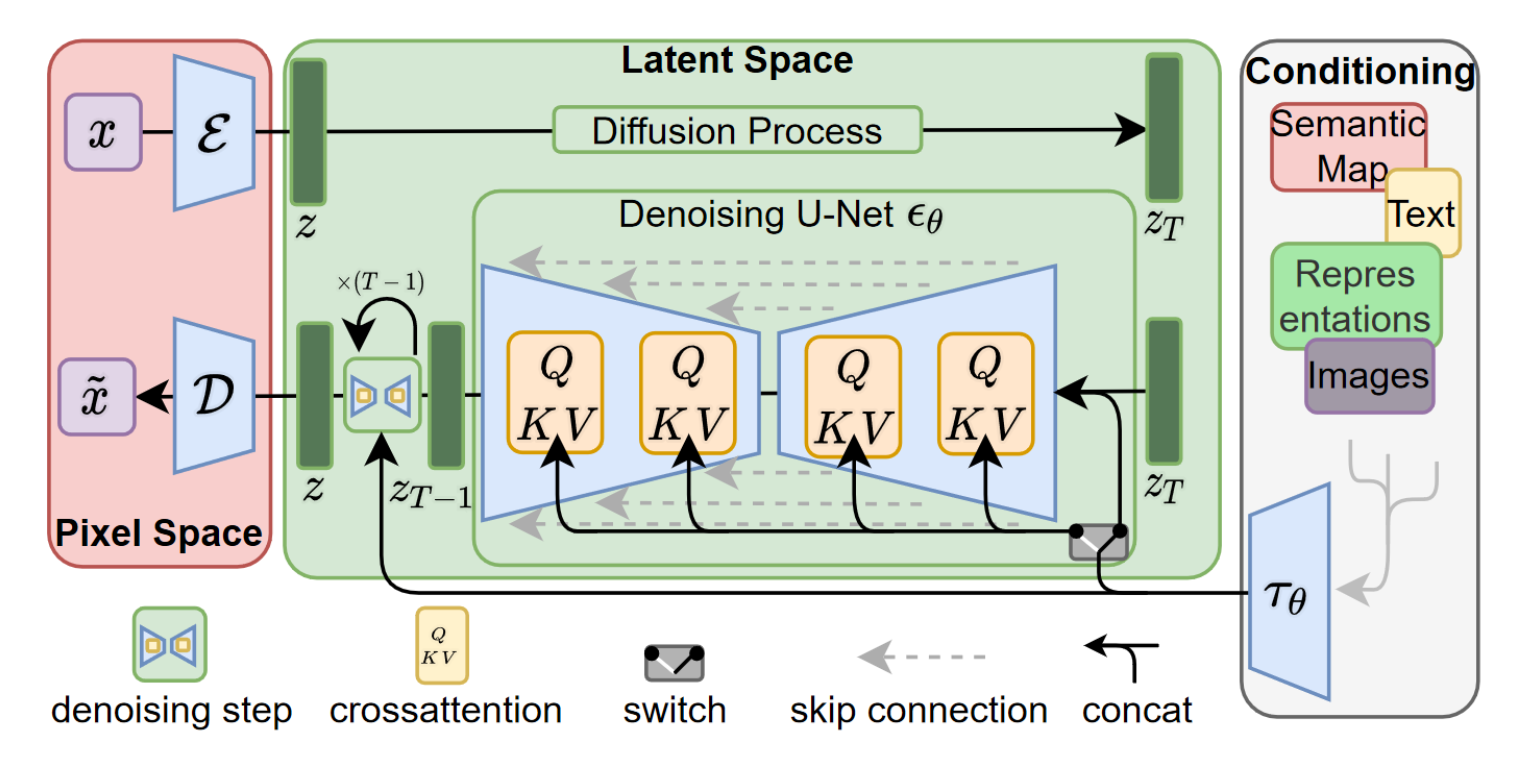
\includegraphics[width=0.9\textwidth]{images/latent-diff.png}
    \caption[Latent Diffusion Model]{Latent diffusion model architecture \cite[Figure 3, p.4]{rombach2022HighResolutionImageSynthesis}}
    \label{fig:latent-diff}
\end{figure}

Thanks to the authors of \cite{rombach2022HighResolutionImageSynthesis} and Huggingface \cite{huggingface2023HuggingFaceAI}, the latent diffusion model was made publicly available and a
pipeline-framework was developed, allowing developers to build upon the existing work easily, test the models locally, and explore and implement new features \cite{huggingface2023DiffusersPipelines}.
This step has led to various community-build diffusion models, ranging from an image-to-image inpainting\footnote{Image-to-image inpainting is a process in computer vision where missing or corrupted parts of an image are filled in with plausible content, usually based on the surrounding context of the image.} diffusion model to a text-to-image diffusion model with multilingual support \cite{huggingface2023CommunityExamples}.

\subsection{Diffusion Probabilistic Models for Tabular Data}
\label{ch:preliminaries-generativeAlgorithms-diffusionProbabilisticModelsTabularData}
At the time of writing, there has been limited work on applying diffusion models to tabular data.
Nevertheless, this section will cover two research papers that apply diffusion to tabular data.

\subsubsection{Diffusion on tabular data imputation}

\textcite{tashiro2021CSDIConditionalScorebased} proposed a conditional score-based diffusion model (CSDI) for the time series imputation task, \ie the task of estimating and filling in missing or absent data points within a time series dataset based on the existing data.
Their CSDI model shows a significant performance increase in generating time-series data compared to other imputation techniques.
\cite{zheng2022DiffusionModelsMissing} showed how the CSDI model can be used in the context of missing value imputation in tabular data that is not a time series (CSDI\_T).
The authors address the problem of simultaneously handling numerical and categorical variables in their work.
Their diffusion model does not reconstruct the complete original data point (\eg an entire tabular data row). 
Instead, the diffusion model receives a splitted version of the input, one part that is observable ("conditional part") $x^{co}$ and one part that is unobservable ("target part") $x^{ta}$.
The goal of the model is, given the unnoised observed part and the noised version of the unobserved part, to return the denoised unobserved part of the next timestep, 
\ie $p_\theta(x^{ta}_{t-1}|x^{ta}_{t},x^{co}_{0})$ \cite{zheng2022DiffusionModelsMissing}.
Categorical entries are converted in three different ways to handle them in conjunction with numerical values.
Categorical values are either \gls{oh} encoded, analog-bits encoded (also called binary encoded), or embedded through a feature tokenization approach proposed by \cite{gorishniy2021RevisitingDeepLearning}.
In the embedding encoding approach, numerical values are encoded as well. 
However, during training, neither the categorical nor the numerical embeddings are learned and remain static and fixed \cite{zheng2023DiffusionModelsMissing}
The authors observed that diffusion achieves competitive results across several datasets for the given evaluation metrics for the task of missing value imputation\footnote{The authors used the \gls{rmse} as well as the error rate as evaluation metric \cite[p. 2]{zheng2023DiffusionModelsMissing}.} \cite{zheng2022DiffusionModelsMissing}.
The different encoding techniques perform comparably well, with the embedding technique outperforming the other two techniques by a slight margin \cite{zheng2022DiffusionModelsMissing}.


\subsubsection{Diffusion on tabular data synthesis}
\label{ch:relatedWork-diffusionModels-tabDDPM}

The task of synthesizing an entire tabular dataset through diffusion has been only explored by \textcite{kotelnikov2022TabDDPMModellingTabular}.
The authors introduce their diffusion model, called TabDDPM, for tabular data synthesis, outperforming the existing state-of-the-art approaches using alternative architectures like \glspl{gan} or \glspl{vae} \cite{kotelnikov2022TabDDPMModellingTabular}. 
Since the TabDDPM approach will be the base for this thesis, it will be explained in detail in this section.

Like \textcite{zheng2022DiffusionModelsMissing}, \textcite{kotelnikov2022TabDDPMModellingTabular} identifies the need for processing categorical variables in some form so that they can be processed by a diffusion model.
However, TabDDPM takes a different approach than the CSDI model, using two different diffusion processes.
The classical Gaussian diffusion process \cite{ho2020DenoisingDiffusionProbabilistic} for numerical columns and multinomial diffusion \cite{hoogeboom2021ArgmaxFlowsMultinomial} (\Autoref{ch:multinomial}) for categorical/binary columns \cite{zheng2022DiffusionModelsMissing}.
Firstly, the feature columns are preprocessed.
Numerical features are transformed using the Gaussian quantile transformation (\Autoref{sec:dataNormalization}), and categorical features are \gls{oh} encoded (\Autoref{sec:dataTransformation}) \cite{kotelnikov2022TabDDPMModellingTabular}.
The objective function is defined as:

\begin{equation}
    \label{eqn:tabddpm_loss}
    \begin{align*}
        L^{TabDDPM}_{t} =L^{simple}_t + \frac{\sum_{i \leq C}^{}L^i_{t}}{C}
    \end{align*}
\end{equation}

where $L^{simple}_t$ is equivalent to \Autoref{eqn:l_simple}, the simplified loss function from \textcite{ho2020DenoisingDiffusionProbabilistic} and $L^i_{t}$ being the \gls{kl}-divergence for each multinomial diffusion term ($L_{t-1}$ in \Autoref{eqn:vlb3}) divided by the number of categorical features $C$ \cite{kotelnikov2022TabDDPMModellingTabular}.

The neural network used to predict the noise in the reverse process is a simple \gls{mlp} based upon the works of \cite{gorishniy2021RevisitingDeepLearning}.
The architecture consists of several identical \gls{mlp}-blocks comprising a Linear layer, followed by an activation layer (\gls{relu}), and a final dropout layer. 
As in \cite{nichol2021ImprovedDenoisingDiffusion, dhariwal2021DiffusionModelsBeat}, the authors combine the input $x_{in}$ with a sinusoidal temporal embedding\footnote{An encoding of the current timestemp in the diffusion process, computed using the mathematical sine function.} and a class label embedding.
Firstly, the input is sent through a linear layer and combined with the temporal and class label embeddings.
The output of that process is sent through a specified number of identical \gls{mlp}-blocks specified above before passing a last linear layer \cite{kotelnikov2022TabDDPMModellingTabular}.

TabDDPM is compared against several baseline models including TVAE \cite{xu2019ModelingTabularData}, CTABGAN \cite{zhao2021CTABGANEffectiveTablea}, CTABGAN+ \cite{zhao2022CTABGANEnhancingTabular},
and a classical interpolation-based approach \gls{smote} \cite{chawla2002SMOTESyntheticMinority}.
Fifteen datasets have been used for generating synthetic data, of which six have a regression task type, seven are binary classification tasks, and two are multiclass classification tasks \cite{kotelnikov2022TabDDPMModellingTabular}.
Eight of the datasets have numerical and categorical features, and seven only consist of numerical features \cite{kotelnikov2022TabDDPMModellingTabular}.
The overall number of features in the datasets varies heavily. 
For a complete list of all datasets, please refer to "Table 2" in \cite[p. 5]{kotelnikov2022TabDDPMModellingTabular}.

The primary evaluation metric chosen by the authors is the machine learning efficacy (see \Autoref{ch:preliminaries-machineLearningEfficacy}).
\textcite{kotelnikov2022TabDDPMModellingTabular} realizes this in three different ways, firstly, by using a set of machine and deep learning models\footnote[5]{Decision Tree, Random Forest, Logistic Regression, \gls{mlp}.} and averaging their performance,
secondly, using a CatBoost model \cite{prokhorenkova2018CatBoostUnbiasedBoosting}(a state-of-the-art model on tabular tasks) \cite{kotelnikov2022TabDDPMModellingTabular}, and thirdly, an \gls{mlp} architecture proposed by \cite{gorishniy2021RevisitingDeepLearning}.
In the latter case, the models are previously tuned on the real dataset so that the best hyperparameters can be found for each dataset, which will be used during the evaluation \cite{kotelnikov2022TabDDPMModellingTabular}.
To account for other random factors that could influence the results, the authors compute the machine learning efficacy metric scores by generating five different synthetic datasets and train the evaluation models for ten random initializations.
The average over all these 50 variations is reported (\cite[Table 3, 4, p. 8]{kotelnikov2022TabDDPMModellingTabular}) including the standard deviation across the metric results \cite{kotelnikov2022TabDDPMModellingTabular}.
\newpage
\noindent The authors summarize three major findings \cite{kotelnikov2022TabDDPMModellingTabular}:
\begin{itemize}
    \item TabDDPM outperforms TVAE and CTABGAN+ on most datasets.
    \item The classical approach\gls{smote}shows surprisingly competitive performance.
    \item The authors contend that the second evaluation protocol, which employs a state-of-the-art model such as CatBoost, is more suitable for calculating the machine learning efficacy, 
    despite the prevalent use of the first protocol in prior works. 
    The firstly mentioned set of models\footnote[5]{Decision Tree, Random Forest, Logistic Regression, \gls{mlp}.} shows overall lower metric scores compared to the CatBoost model.
    Thus, the authors argue the set of other models'\footnotemark[5] performance values are of lower relevance for practitioners, who, in real-world scenarios, are rather interested in using state-of-the-art models rather than suboptimal models.
    Additionally, for the set of models, the models trained on synthetic data outperformed the models trained on actual real data, indicating that the 
    synthetic data is "more valuable than the real" data, which should not be the case \cite[p. 8]{kotelnikov2022TabDDPMModellingTabular}.
    This behavior cannot be observed if tuned \gls{mlp} or CatBoost models are used for evaluation \cite{kotelnikov2022TabDDPMModellingTabular}.
\end{itemize}

Additionally, the authors provide a small comparison based on distribution plots and correlation matrices.
In their comparison, they show that the produced feature distribution plots by TabDDPM for a selected number of columns of different datasets look more similar 
to the real distributions, compared to plots produced by CTABGAN+ or TVAE \cite{kotelnikov2022TabDDPMModellingTabular}.
The authors argue that this observation is consistent for numerical, categorical, and mixed data type columns \cite{kotelnikov2022TabDDPMModellingTabular}.
The pairwise correlation matrices difference plots (performed similarly to in \cite{brenninkmeijer2019GenerationEvaluationTabular}) show a smaller difference between the synthetic and real data for the TabDDPM model compared to CTABGAN+ and TVAE.
Since the TabDDPM model show more realistic correlation difference plots for multiple datasets, 
the authors assert that this demonstrates that their TabDDPM model exhibits greater flexibility than other alternatives and generates synthetic data of higher quality \cite{kotelnikov2022TabDDPMModellingTabular}.

Lastly, \cite{kotelnikov2022TabDDPMModellingTabular} performs a privacy evaluation against the\gls{smote}approach.
The median \gls{dcr} is, which calculates the minimum Euclidean distance to real data points for each synthetic sample \cite{zhao2021CTABGANEffectiveTable}.
Small \glspl{dcr} point towards mere copying of data samples (overfitting), while high values indicate actual new synthetic data samples \cite{kotelnikov2022TabDDPMModellingTabular}.
The results presented by the authors show a higher \gls{dcr} score for TabDDPM for all datasets compared to\gls{smote}while having a similar or higher machine learning efficacy score \cite{kotelnikov2022TabDDPMModellingTabular}.

To summarize, the TabDDPM approach is a novel way to generate synthetic data of high utility using Gaussian and multinomial diffusion.
TabDDPM outperforms other state-of-the-art baseline models in terms of machine learning efficacy on multiple datasets.
Moreover, distributions and correlations produced from synthetic data by TabDDPM look more similar to those of the real data than synthetic data produced by other models.






\chapter{Conceptual Design}
\label{ch:conceptualDesign}

\section{Requirements}
\label{ch:conceptualDesign-requirements}

% Ähnlich wie bei Masterarbeit "Generierung einer synthetischen Datenhistorie aus einem Datenbank Snapshot"
% Basierent auf ISO 2510 
% Nicht Funktional: Functional Suitability, Maintainability, (Compatibility (reproducability))

% Funktional (ergeben sich aus den Research Questions):
% - Comparability & reproducability (codebase must be able to reproduce existing results)
% - "Special Processing": must be able to handle tabular data as explained in chapter xy
% - "Special Processing": can have multiple versions (bayesian, embedding, etc.) 
% - "Special Processing": different versions should be switchable easily
% - "Special Processing": Provide general framework for possible future special processing types
% - Evaluation: must be able to evaluate the results with statistical similarity measures

- gans struggled with generating discrete variables \cite{torfi2020CorGANCorrelationCapturingConvolutionala}
- remarkable performance generating syntehtic images and time series data \cite{mckeever2020SynthesisingTabularDatasets}
- struggle with mode collapse --> generate same sample \cite{torfi2020CorGANCorrelationCapturingConvolutionala}

\section{Existing Code Base}
\label{ch:conceptualDesign-existingCodeBase}

\subsection{Current Implementation}
\label{ch:conceptualDesign-existingCodeBase-currentImplementation}
% Why did I choose to use the existing code base?
% What are the advantages and disadvantages of the existing code base?
% Diagram explaining the current Software architecture

\subsection{Experiment Run}
\label{ch:conceptualDesign-existingCodeBase-experimentRun}
% What is an experiment run? (train, sample, evaluate, hyperparameter tuning, ...)
% Diagrams explaining the current implementation 
% Hyperparameters

\subsection{Reproduction of existing Results}
\label{ch:conceptualDesign-existingCodeBase-reproductionOfExistingResults}
% Reproduce the results of the paper "Diffusion Probabilistic Models for Tabular Data Synthesis"

\section{Proposed Code Extensions}
\label{ch:conceptualDesign-codeExtensions}

\subsection{"Special Processing"}
\label{ch:conceptualDesign-codeExtensions-dataPreprocessing}

\cite{borisov2022DeepNeuralNetworks} provides a taxonomy for data learning for tabular data with "data transformation methods" into "single dim encodings" and "multi dim encodings" 
--> Approaches in diese taxonomy einordnen

% what is meant with "special processing"? --> transforming the data into a different format
% what is necessary to consider when transforming the data? --> Only fit on train data not on test data, etc. 
% why is it necessary? --> to improve the results
% how is it implemented? --> Processing abstract class with different implementations

% Details for each processing type? or later?

\subsection{Evaluation}
\label{ch:conceptualDesign-codeExtensions-evaluation}

% How and where is the statistical similarity measured? 

\subsection{Experiment Run}
\label{ch:conceptualDesign-codeExtensions-experimentRun}

% How did the Experiment Run change with the code extensions?
% Hyperparameters

\section{Experiments}

% What experiments with which changes are planned?
% Baseline 1: no preprocessing + statistical similarity
% Baseline 2: Other Data Generation algorithms (GAN, ...) + statistical similarity 
% Experiment 1.1: preprocessing Bayesian gaussian mixture + statistical similarity
% Experiment 2.1: preprocessing embeddings + statistical similarity
% ...
% Experiment N: Baseline 1 + hyperparameter optimization based on statistical similarity
% if Experiment N > Baseline 1:
%   Experiment 1.2: preprocessing Bayesian gaussian mixture + hyperparameter optimization based on statistical similarity
%   Experiment 2.2: preprocessing embeddings + hyperparameter optimization based on statistical similarity
%   ...
\chapter{Methodology}
\label{ch:methodology}

This section delves into the methodology employed to address the research questions and objectives outlined in the previous chapters.
The chapter is organized into three main sections.
\autoref{ch:architecture} discusses the architecture of our proposed solution, elaborating on the tabular processor and its implementations, namely the BGMProcessor and FTProcessor.
In addition, this section also highlights the modifications made to the existing software to incorporate the proposed solutions.

\autoref{ch:methods-experimentalSetup} focuses on the experimental setup, outlining the experiments conducted to evaluate the performance and effectiveness of the proposed models.
It provides detailed information on the execution environment and the hyperparameter search space used in the study, ensuring the reproducibility of the results.

Finally, \autoref{ch:methods-datasets} presents the dataset utilized in the experiments, including its source and characteristics.
This information is crucial to understanding the context in which our proposed methodology was tested and evaluated.

By the end of this chapter, the reader will gain a comprehensive understanding of the methodology implemented in this thesis, which will lead to the presentation and analysis of the results in the subsequent chapters.

\section{Architecture}
\label{ch:architecture}

The software's architecture was developed with the requirements in \autoref{ch:requirements} in mind.
The following section will explain how the individual additions to the existing code are designed and why the design was chosen.


\subsection{Tabular Processor}
\label{ch:architecture-tabularProcessor}

To allow for flexible use and the possibility of adding additional processing mechanisms (R5 - Maintainability), the \textit{strategy design} pattern (\autoref{fig:design}) was chosen \cite{gamma1994design}.
The pattern is beneficial if a specific behavior is required, but needs to be realized in different ways.
The \textit{Strategy} class defines what kind of methods need to be implemented and what behavior the class should have.
The \textit{Strategy} classes children define a \textit{ConcreteStrategy} and realize the desired behavior in different ways.
Different \textit{ConcreteStrategies} can be used interchangeably independent of the \textit{Context} they are used in since all implement the same functionalities.
Additionally, new \textit{ConcreteStrategies} can be added easily without affecting any of the other \textit{ConcreteStrategy} or the \textit{Context} \cite{gamma1994design}.

\begin{figure}[h]
	\centering
	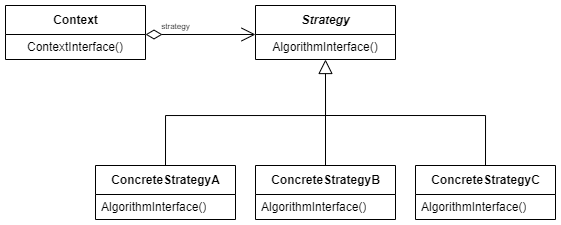
\includegraphics[width=0.8\textwidth]{images/strategy.png}
	\caption[Strategy Design Pattern]{Strategy design pattern \cite[p. 316]{gamma1994design}}
	\label{fig:design}
\end{figure}

\begin{figure}[h]
	\centering
	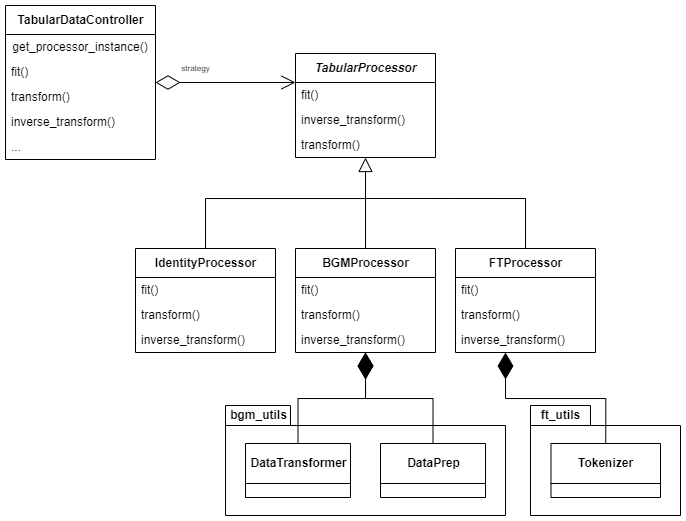
\includegraphics[width=0.8\textwidth]{images/tabular_processor.png}
	\caption[Tabular Processor Design]{Tabular Processor Design}
	\label{fig:tabular_processor}
\end{figure}

\autoref{fig:tabular_processor} shows how the \textit{Strategy} design pattern is realized.
The overall \textit{Strategy} is defined in the \textit{TabularProcessor} class in the form of an abstract class with three core methods each tabular processing mechanism needs to implement.
These functions are the \textit{fit}, \textit{transform}, and \textit{inverse transform} functions (FR2.1 - FR2.3).

Each different tabular processing strategy is different and realizes the transformation of the data in a different way by implementing the abstract functions of the parent strategy.
Therefore, new tabular processing mechanisms can be easily added by just implementing the methods of the abstract class (R2, FR2).
Furthermore, the tabular processing mechanism can be exchanged easily since they share the same functions.
This is handled in the \textit{TabularDataController} class, equivalent to the \textit{Strategy} design pattern \textit{Context}.
The \textit{TabularDataController} handles all relevant aspects to use the tabular processing mechanisms, including but not limited to the instantiation, fitting, saving, and loading of \textit{TabularProcessor} instances.
The data, whose columns are separated into categorical, numerical, and target as numpy arrays \cite{harris2020array}, needs to be provided to instantiate a tabular processor.
Target refers to the column of the dataset that a model tries to predict or estimate in a classification or regression scenario.
The first step in using the tabular processor is fitting it to the data.
Additional information required for the fitting process can be provided through meta-data in the form of a dictionary, which may change for different realizations.
Note that this fit function might not be necessary, depending on the processing mechanism, but it is required to be implemented anyways.
Only after fitting the transform function can be called, transforming the data and returning the transformed data in the same format.
The inverse transformation works similarly, reversing transformed data back to its original format.


\subsection{Tabular Processor Implementations}
\label{ch:architecture-tabularProcessor-implementations}

Three different tabular processor versions have been implemented.
The \textit{IdentityProcessor} does not do anything to the data.
It is used to do experiments without any tabular processing mechanism and allows reproducing the original results of \cite{kotelnikov2022TabDDPMModellingTabular}.
In this thesis, only two approaches have been implemented, the \gls{bgm} and \gls{ft} tabular processors.
Other potential tabular processing mechanisms have been considered but usually lack one of the specified criteria in \autoref{ch:Concept-criteria}.
The biggest challenge usually is the reversibility, since there are several encoding strategies that only work with the encoded version of the data.
Consequently, they do not require decoding the encoded data and are, therefore, not implemented.
A decoding mechanism could be invented for each process that does not have one already.
However, this would exceed the scope of this thesis, as it would be very complex and time-consuming and remains an open task for future researchers.

\subsubsection{BGMProcessor}
\label{ch:BGMProcessor}

The BGMProcessor is the same processing mechanism that has been introduced by the CTABGAN+ model \cite{zhao2022CTABGANEnhancingTabular}.
This processing mechanism was chosen since it fulfills all criteria mentioned in \autoref{ch:Concept-criteria}.
Moreover, it is part of a state-of-the-art tabular data synthesis \gls{gan}-based model, which has already proven successful.

Firstly, a mixed-type encoding is introduced, specifically designed to encode single columns containing a mixed data type of numerical and categorical data types.
For the continuous values in the column, the authors adapt the mode-specific normalization technique from \cite{xu2019ModelingTabularData} using a \gls{bgm} implementation \cite{scikit-learndevelopers2023BayesianGaussianMixture}, which is a \gls{vgm} (see \autoref{sec:dataNormalization} for details).
For the categorical values, the $\beta$ \gls{oh} vector is extended by the number of possible categorical values in the column.
If a categorical value should be encoded, the $\alpha$ value is set to 0, and the \gls{oh} encoding indicating the specific category is set to 1.
Additionally, the authors allow missing values, which are treated as another categorical entry.

Furthermore, the authors introduce a "general transform" mechanism \cite[p. 7]{zhao2022CTABGANEnhancingTabular} that is supposed to be used for simple distributions and counters the problem of exploding dimensionality caused by a \gls{oh} encoding \cite{zhao2022CTABGANEnhancingTabular}.
This general transformation is mapping the values into a range of [-1, 1], which is achieved through a shifted and scaled min-max normalization (see min-max scaler in \autoref{sec:dataNormalization}).
Mathematically, the encoded datapoint $x^t_i$ can be computed using the original datapoint $x_i$ in column $x$ through the following formula:
\begin{equation}
	\begin{align*}
		x^t_i=2* \frac{x_i-\min(x)}{\max(x)-\min(x)}-1
	\end{align*}
\end{equation}
Which can easily be reversed in the following way:
\begin{equation}
	\begin{align*}
		X_i = (\max(x)-\min(x))*\frac{X^t_i+1}{2}+\min(x)
	\end{align*}
\end{equation}
Categorical values are label encoded before applying the normalization \cite{zhao2022CTABGANEnhancingTabular}.
The authors observe that this simplistic general transformation for continuous values only works well for simple distributions (\eg single-mode gaussian) and not for complex distributions, for which the mode-specific normalization is preferred \cite{zhao2022CTABGANEnhancingTabular}.
For categorical values, the general transformation should only be applied if the number of categories a column can take is very high and would lead to very sparse vectors that make computation complex \cite{zhao2022CTABGANEnhancingTabular}.
Lastly, the authors log-transform columns that suffer from very long tails (see \autoref{sec: synthetic tabular data generation}) because \Glspl{bgm} seem to have difficulties encoding values towards the tail \cite{zhao2022CTABGANEnhancingTabular}.
The log-transformation of each value $\tau$ in the column will be compressed to $\tau^e$, given a lower bound $l$ using:
\begin{equation}
	\label{eqn:log-transform}
	\begin{align*}
		\tau^e =
		\begin{cases}
			log(\tau)            & \text{if } l>0                                 \\
			log(\tau-l+\epsilon) & \text{if } l\leq0 \text{, where } \epsilon > 0
		\end{cases}
	\end{align*}
\end{equation}

This encoding strategy is realized in the BGMProcessor class, which uses the DataPrep and DataTransformer class, as developed by \cite{zhao2022CTABGANEnhancingTabular}.
These classes require additional information about the dataset, provided by the user, including what columns are categorical, categorical columns that have a high cardinality/dimensionality\footnote{Inside the code of the authors, they refer to it as "non\_categorical\_columns", which is a bit misleading. Categorical columns with high dimensionality are transformed into numerical columns and handled as if they were continuous.},
numerical, mixed (including what values are categorical), as well as what columns require a log transformation and which a general transformation.
This information is provided to the \textit{BGMProcessor} by extending the info.json (\autoref{lst:info}) with an additional entry, \textit{dataset\_config}, see \autoref{lst:info_extended} for an example.

\begin{lstlisting}[label={lst:info_extended},caption={Example extended data info file from the adult dataset (\autoref{ch:methods-datasets})}]
    {
    "name": "Adult",
    [...]
    "val_size": 6513,
    "dataset_config": {
        "cat_columns": [ // categorical columns
            "workclass", 
            (...), 
            "income"
            ],
        "non_cat_columns": [], // high dim-categorical
        "log_columns": [], // log-transformation
        "general_columns": [ //  general-transformation
            "age"
            ], 
        "mixed_columns": { // mixed-data-types
            "capital-loss": [0.0], // the "0.0" value is categorical           
            "capital-gain": [0.0]
            },
        "int_columns": [ // numerical columns 
            "age", 
            (...), 
            "hours-per-week"
        ],
        "problem_type": "binclass", // [binclass|multiclass|regression]
        "target_column": "income"
        }
    }
\end{lstlisting}

\subsubsection{FTProcessor}
\label{ch:FTProcessor}

The \textit{FTProcessor}, short for \textit{Feature Tokenization Processor}, is based upon the work of Zheng \etal \cite{zheng2022DiffusionModelsMissing} and Gorishniy \etal \cite{gorishniy2021RevisitingDeepLearning}.
Similar to the \gls{bgm} variant, it fulfills all criteria stated in \autoref{ch:Concept-criteria}.
However, the \gls{ft} mechanisms have only been used in a data imputation task, where only individual cells must be synthesized.
It is unclear whether its functionality can be extended to multiple-cell synthetisation.

The \gls{ft} transforms tabular data into a static embedding representation.
Categorical columns are embedded through an embedding layer, which is basically a look-up table \cite{pytorch2023EmbeddingPyTorch13} of fixed size.
Each categorical input tensor of dimensions $[N]$ (\ie a table with $N$ columns) will be transformed in an embedding of size $[N,H]$ with $H$ as the embedding dimensionality \cite{gorishniy2021RevisitingDeepLearning}.
Numerical columns will be processed by a simple multiplication of linear layers weights \cite{gorishniy2021RevisitingDeepLearning}.
Lastly, a bias term is added to both categorical and numerical columns.
\autoref{fig:ft} illustrates how a tabular data row with three numerical and two categorical features could be transformed into a new tensor \cite[Figure 2a, p.4]{gorishniy2021RevisitingDeepLearning}.

\begin{figure}[h]
	\centering
	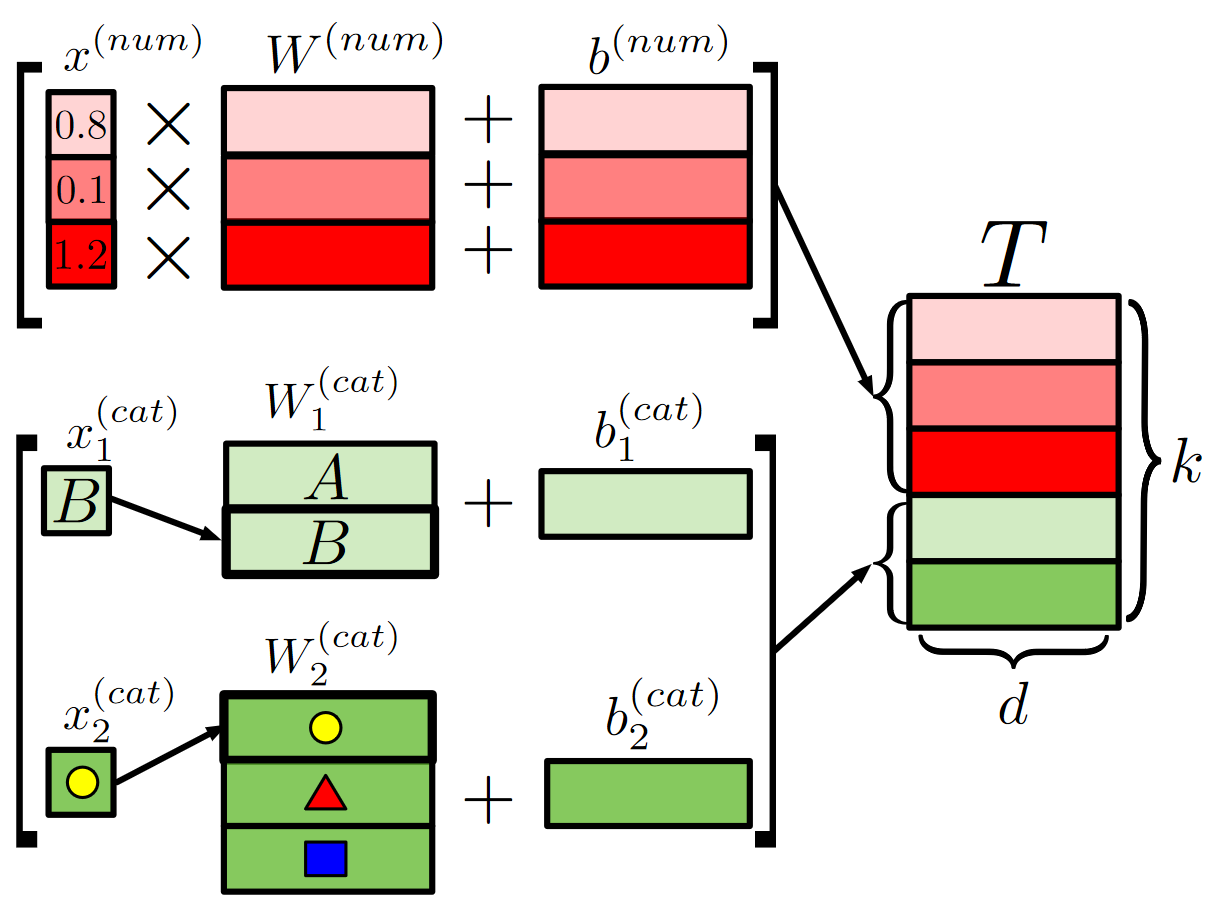
\includegraphics[width=0.5\textwidth]{images/ft.png}
	\caption[Feature Tokenization]{Feature Tokenization \cite[Figure 2a, p.4]{gorishniy2021RevisitingDeepLearning}}
	\label{fig:ft}
\end{figure}

To revert the data that the diffusion model produces to the original data format, the numerical and categorical columns need to be handled differently.
The corresponding embedding weights divide the numerical output element-wise, and the average value is computed as the final output \cite{zheng2022DiffusionModelsMissing}.
For categorical output, the closest categorical embedding is determined by computing the euclidean distance between the produced output and every categorical embedding \cite{zheng2022DiffusionModelsMissing}.

In the original work of \cite{gorishniy2021RevisitingDeepLearning}, the feature tokenizer is directly in front of a transformer model, allowing the gradients to flow through the embedding and linear layers during training.
This enables the model to learn a meaningful embedding.
In the adaptation of \cite{zheng2023DiffusionModelsMissing} and in this thesis, the weights of the layers are frozen.
Hence, learning is not possible, and the embedding is static.
In this thesis, the data transformation and the actual model training are fully separated,
resulting in gradients not flowing back to the feature tokenizer to update any weights of the embeddings.

\subsection{Changes to the existing software}
\label{ch:methods-changes}
The changes to the existing software (\autoref{ch:conceptualDesign-existingCodeBase}) are various and include multiple major changes as well as a lot of small changes.
Below, the major changes to the individual script are listed.
Additional visualization of the process of the scripts can be found in \autoref{A:activity_diagrams}

\begin{description}
	\item[train.py:]
		Before the dataset is preprocessed and transferred into a dataset class, the TabularDataController handles the tabular processing mechanisms.
		For this, a TabularDataController is instantiated at the beginning and either loads a previously fit TabularProcesser instance or fits and saves the TabularProcesser on the training data.
		It receives context information on which tabular processing mechanisms and which properties the dataset has through the configuration file and handles the
		instantiation, fitting, and transformation of the raw data.
		Despite the addition of the TabularDataController, the actual training remained untouched.
		Hence, introducing a TabularProcesser only changes the data format the diffusion model will receive and does not change the actual training loop.

	\item[sample.py:]
		A TabularDataController is instantiated at the beginning and loads a previously fit TabularProcesser instance.
		If there is no previous TabularProcesser instance to be loaded, it will call the fit function again.
		After the sampling is finished, the TabularProcesser's inverse transform function is called to bring the synthetic data in the original data format.

	\item[eval\_similarity.py:]
		This script does not replace the previous evaluation script.
		Instead, it is called after the original evaluation script (see \textit{pipeline.py}).
		First, three TabularDataController instances are created, one for each train-, validation- and test data split.
		With the TabularDataController instances, \gls{pd} \cite{mckinney-proc-scipy-2010} data frames are created, which are required for the TabSynDex similarity score.
		After the TabSynDex score is calculated, visualizations are created, if set by the user.

	\item[pipeline\_*.py:]
		The basic pipeline hardly changed.
		The only major change is that the similarity score evaluation is performed after the default evaluation using machine learning efficacy.
		In this evaluation, the TabSynDex metric is calculated as well as (if set by the user) visualization are created.

	\item[tune\_*.py:]
		Inside the tuning script, the objective function changed.
		If set by the user, the objective function will be based on the TabSynDex similarity score instead of the machine learning efficacy.
		To reduce processing time, visualization inside the similarity evaluation part will, by default, only be created after the hyperparameters have been found and the eval\_seeds script will be executed.

	\item[eval\_seeds.py:]
		The basic eval\_seeds script did not change a lot.
		Again, the TabSynDex metric will be called after the default machine learning efficacy.
\end{description}

\section{Experimental Setup}
\label{ch:methods-experimentalSetup}

\subsection{Experiments}
\label{ch:Experiments}

To systematically analyze the performance of the different tabular processing mechanisms, the following baseline experiments have been performed:

\begin{description}
	\item[Baseline-Real:] Comparison of the real training data with the real test data.
		The similarity evaluation is expected to be very high since the data is from the same joint distribution.
		The computed machine learning efficacy score can be seen as an objective value that should be reached.
		The closer the synthetic data based machine learning efficacy results are to this target, the better the synthetic data.
	\item[Baseline-TabDDPM:] Reproduction of the TabDDPM results of the authors \cite{kotelnikov2022TabDDPMModellingTabular} but with the extend evaluation explained in \autoref{ch:conceptualDesign-Evaluation} (Machine learning efficacy + TabSynDex + Visualizations).
	\item[Baseline-TVAE:] Like Baseline-TabDDPM but for TVAE.
	\item[Baseline-CTABGAN:] Like Baseline-TabDDPM but for CTABGAN.
	\item[Baseline-CTABGAN+:] Like Baseline-TabDDPM but for CTABGAN+.
	\item[Baseline-SMOTE:] Like Baseline-TabDDPM but for SMOTE.
\end{description}

\noindent For each implemented Tabular Processing mechanism, the following three experiments should be performed:

\begin{description}
	\item[Experiment 1:] Tabular Processing combined with TabDDPM with additional similarity evaluation. Hyperparameters tuned like in the original experiment (tuned after CatBoost-machine learning efficacy score).
	\item[Experiment 2:] Like Experiment 1, but hyperparameters are optimized towards the TabSynDex similarity score instead of the machine learning efficacy score.
	\item[Experiment 3:] Like Experiment 2, but the preprocessing strategy, that normalizes numerical data after the tabular processing transformation is replaced from a quantile transform function to a min-max transformation or is completely removed.
\end{description}

\noindent Depending on the results of the first experiments, subsequent experiments may only be performed on a subset of promising Tabular processing mechanisms.
To not get confused with the different model versions, the models are named after the following principal:

Modelname[-TabularProcessor]$^{tuning}_{preprocessing}$

The Modelname is followed by an optional tabular processing mechanism.
The tuning strategy ("ml" for "machine learning efficacy score" or "s" for "TabSynDex similarity score") is indicated via a superscript (Experiment 2).
The preprocessing strategy ("q" for "quantile transform" or "m" for "min-max", or "n" for "none"/"no transformation") is indicated via a subscript (Experiment 3).

The min-max strategy was chosen as a commonly used linear transformation counterpart to the non-linear quantile transformation.
Since some tabular processing strategies already normalize or standardize the data, additional quantile or min-max transformations may not be required, which is why experiment 3 will also investigate,
what the effect of having no transformation after the tabular processor is.

\subsection{Execution Environment}
\label{ch:environment}

The code was developed in python version 3.9.7 and made use of several libraries.
Most important libraries include (for a full list, please see the \textit{environment.yml} file in the source code):
\begin{itemize}
	\item azure-core, azureml-core: For running the code in the Microsoft Azure cloud \cite{microsoft2023CloudComputingServices}.
	\item catboost (1.0.3): contains the CatBoost model for the machine learning efficacy.
	\item pytorch (1.10.1): neural network framework.
	\item table\_evaluator (1.4.2): used to produce visualizations.
	\item numpy (1.21.4): allows efficient array computing.
	\item optuna (2.10.1): used for hyperparameter tuning.
	\item pandas (1.5.2): allows fast computing with dataframes of tabular data.
	\item scikit-learn (1.0.2): includes several utility functions for machine learning, \eg metrics.
	\item TabSynDex \cite{chundawat2022UniversalMetricRobusta}: TabSynDex metric source code.
\end{itemize}

The training was performed using Microsoft Azure Machine Learning Studio.
Each experiment was executed on a STANDARD\_NC6 compute cluster running on Linux distribution, consisting of six virtual \glspl{cpu} (Intel Xeon E5-2690v3) with 56 GB Memory, 340 GB (SSD) Storage and the computing of one-half \gls{gpu} (Tesla K80) with 12 GB \gls{gpu} memory \cite{vikancha-msft2022NCseriesAzureVirtual}.
All experiments could also be performed locally on a Windows machine using a \gls{cpu}.
Local experiments with a \gls{gpu} should be possible but have not been tested.

\subsection{Hyperparameters}
The hyperparameter search space for the various models was not changed and is equal to the experiments in \cite{kotelnikov2022TabDDPMModellingTabular}.
\begin{table}[h]
	\centering
	\begin{tabular}{lr}
		\toprule
		Parameter                 & Distribution        \\
		\midrule
		Max depth                 & UniformInt[3, 10]   \\
		Learning rate             & LogUniform[1e-5, 1] \\
		Bagging temperature       & Uniform[0,1]        \\
		L2 leaf reg               & LogUniform[1,10]    \\
		Leaf estimation iteration & UniformInt[1,10]    \\
		\midrule
		Number of tuning trials   & 100                 \\
		\bottomrule
	\end{tabular}
	\caption[CatBoost Hyperparameter Search Space]{CatBoost evaluation model hyperparameter tuning search space (proposed by \cite{gorishniy2021RevisitingDeepLearning})}
	\label{tab:catboost_tune}
\end{table}

\begin{table}[h]
	\centering
	\begin{tabular}{lr}
		\toprule
		Parameter               & Distribution                       \\
		\midrule
		Learning Rate           & LogUniform[1e-5,3e-3]              \\
		Batch Size              & Cat\{256,4096\}                    \\
		Diffusion timesteps     & Cat\{100,1000\}                    \\
		Training iterations     & Cat\{5000,10000,20000\}            \\
		\# MLP layers           & Int\{2,4,6,8\}                     \\
		MLP layer width         & Int\{128,256,512,1024\}            \\
		Proportion of samples   & Float\{0.25, 0.5, 1, 2\}           \\
		\midrule
		Train size              & \#entries in training dataset      \\
		\# Samples              & Proportion of samples * Train size \\
		Dropout                 & 0.0                                \\
		Scheduler               & cosine                             \\
		Gaussian diffusion loss & mse                                \\
		\midrule
		Number of tuning trials & 100                                \\
		\bottomrule
	\end{tabular}
	\caption[TabDDPM Hyperparameter Search Space]{TabDDPM model hyperparameter tuning search space}
	\label{tab:diff_tune}
\end{table}



\begin{table}[h]
	\centering
	\begin{tabular}{lr}
		\toprule
		Parameter               & Distribution                     \\
		\midrule
		\# classif. layers      & UniformInt[1,6]                  \\
		Classif. layer size     & Int\{62, 128, 256, 512\}         \\
		Training itertations    & Cat\{5000, 20000, 30000\}        \\
		Batch size              & Cat\{456,4096\}                  \\
		Embedding dim.          & Int\{16,32,64,128,256,512,1024\} \\
		Loss factor             & LogUniform[0.01, 10]             \\
		Proportion of samples   & Float\{0.25, 0.5, 1, 2, 4, 8\}   \\
		\midrule
		Number of tuning trials & 100                              \\
		\bottomrule
	\end{tabular}
	\caption[TVAE Hyperparameter Search Space]{TVAE model hyperparameter tuning search space}
	\label{tab:tvae_tune}

\end{table}

\begin{table}[h]
	\centering
	\begin{tabular}{lr}
		\toprule
		Parameter               & Distribution                   \\
		\midrule
		\# classif. layers      & UniformInt[1,4]                \\
		Classif. layer size     & Int\{62, 128, 256\}            \\
		Training itertations    & Cat\{1000, 5000, 7500\}        \\
		Batch size              & Int\{512,1024,2048\}           \\
		random dim.             & Int\{16,32,64,128\}            \\
		\# Channels             & Int\{16, 32, 64\}              \\
		Proportion of samples   & Float\{0.25, 0.5, 1, 2, 4, 8\} \\
		\midrule
		Number of tuning trials & 30                             \\
		\bottomrule
	\end{tabular}
	\caption[CTAGBAG(+) Hyperparameter Search Space]{CTAGBAG/CTABGAN+ model hyperparameter tuning search space. Training iterations and the number of tuning trails were reduced compared to the original \cite{kotelnikov2022TabDDPMModellingTabular}, to reduce computation time.}
	\label{tab:ctabgan_tune}
\end{table}

\section{Dataset}
\label{ch:methods-datasets}

The dataset that was used for experiments is the \textit{Adult} dataset, also known as "Census Income" from the UCI Machine Learning repository \cite{Dua:2019}.
The dataset was constructed through an extraction from a 1994 census database \cite{kohavi1996ScalingAccuracyNaiveBayes}.
Overall, the dataset has 15 columns, of which nine are categorical, and six are continuous, and has 48842 rows.

The continuous columns are:


\textit{age}, \textit{fnlwgt}\footnote{short for "final weight", a sampling weight}, \textit{education-num}, \textit{capital-gain}, \textit{capital-loss} and \textit{hours-per-week}


And the categorical columns are:


\textit{workclass}, \textit{education}, \textit{marital-status}, \textit{occupation}, \textit{relationship}, \textit{race}, \textit{sex}, \textit{native-country} and \textit{income} (target column)



The dataset was created for binary classification, where the model should predict the column value of the income column (either \textit{>50K} or \textit{<=50K}).

\autoref{tab:adult} shows five entries of the dataset:


\begin{table}[h]
	\centering
	\resizebox{\columnwidth}{!}{
		\begin{tabular}{|c|c|c|c|c|c|c|c|c|c|c|c|c|c|c|}
			\toprule
			\textbf{age} & \textbf{workclass} & \textbf{fnlwgt} & \textbf{education} & \textbf{education-num} & \textbf{marital-status} & \textbf{occupation} & \textbf{relationship} & \textbf{race} & \textbf{sex} & \textbf{capital-gain} & \textbf{capital-loss} & \textbf{hours-per-week} & \textbf{native-country} & \textbf{income} \\
			\midrule
			39.0         & State-gov          & 77516.0         & Bachelors          & 13.0                   & Never-married           & Adm-clerical        & Not-in-family         & White         & Male         & 2174.0                & 0.0                   & 40.0                    & United-States           & $\leq$50K       \\
			50.0         & Self-emp-not-inc   & 83311.0         & Bachelors          & 13.0                   & Married-civ-spouse      & Exec-managerial     & Husband               & White         & Male         & 0.0                   & 0.0                   & 13.0                    & United-States           & $\leq$50K       \\
			38.0         & Private            & 215646.0        & HS-grad            & 9.0                    & Divorced                & Handlers-cleaners   & Not-in-family         & White         & Male         & 0.0                   & 0.0                   & 40.0                    & United-States           & $\leq$50K       \\
			53.0         & Private            & 234721.0        & 11th               & 7.0                    & Married-civ-spouse      & Handlers-cleaners   & Husband               & Black         & Male         & 0.0                   & 0.0                   & 40.0                    & United-States           & $\leq$50K       \\
			28.0         & Private            & 338409.0        & Bachelors          & 13.0                   & Married-civ-spouse      & Prof-specialty      & Wife                  & Black         & Female       & 0.0                   & 0.0                   & 40.0                    & Cuba                    & $\leq$50K       \\
			\bottomrule
		\end{tabular}
	}
	\caption[Example Adult Dataset]{Adult income dataset with five exemplary entries}
	\label{tab:adult}
\end{table}




\chapter{Results}
\label{ch:results}

In this chapter the results from the previous in \Autoref{ch:methodology} introduced experiments are presented.
Firstly, \Autoref{ch:results-reproduction} deals with a reproduction and a verification of the results achieved by \textcite{kotelnikov2022TabDDPMModellingTabular}.
Subsequently, \Autoref{ch:results-Metric-results} will present the numerical metric results of the experiments that have been outlined in \Autoref{ch:methodology}.
These include the metric results from the machine learning efficacy scores, as well as the TabSynDex similarity score metrics.
\Autoref{ch:results-Visual} will present selected visual results from the executed experiments, highlighting important characteristics and observations made from the synthetic data that has been generated.
All of this provides the basis for \Autoref{ch:results-discussion}, which analyses and interprets the numerical and visual results from the previous sections.
This section will also revisit and answer the research questions of this thesis from \Autoref{ch:intro-goals} according to the gathered data.
Lastly, this chapter will finish with \Autoref{ch:results-limitations}, critically assessing the constraints and limitations of the study, taking into account the data use, experimental scope, and \gls{model} interpretability.

\section{Reproduction and Verification of Results}
\label{ch:results-reproduction}

Given that this thesis draws heavily upon the research conducted by \cite{kotelnikov2022TabDDPMModellingTabular},
it was deemed necessary to first reproduce the original experiments and subsequently verify the authors' findings,
prior to conducting any new experiments.
Fortunately, the publicly available code \cite{akim2023TabDDPMModellingTabular} facilitated the replication of the experiments with relative ease.

The reproduction is limited to the adult dataset from \Autoref{ch:methods-datasets} and to the machine learning efficacy computed with a tuned CatBoost \cite{prokhorenkova2018CatBoostUnbiasedBoosting} \gls{model}.

Firstly, a CatBoost \gls{model} was tuned on the adult dataset using the provided tuning script (tune\_evaluation\_model.py).
Next, for each sampling algorithm, a \gls{model} was trained according to the configuration files provided by the authors.
Each configuration file contains the parameter settings the authors identified during hyperparameter tuning.
Hence, with the models' respective pipeline.py script, the best-found \gls{model} from hyperparameter tuning could be trained and saved.
Finally, the trained CatBoost and trained sampling \gls{model} were used in the evaluation script (eval\_seeds.py), which calculates and reports the results.

\begin{table}[h]
	\centering
	\begin{tabular}{lccr}
		\toprule
		\textbf{Model}     & \textbf{Reproduction} & \textbf{Original} & \textbf{Difference} \\
		\midrule
		Real               & 0.815                 & 0.815             & 0                   \\
		TVAE$^{ml}$        & 0.780                 & 0.781             & -0.001              \\
		CTABGAN$^{ml}$     & 0.775                 & 0.783             & -0.008              \\
		CTABGAN+$^{ml}$    & 0.775                 & 0.772             & +0.003              \\
		SMOTE$^{ml}$       & 0.791                 & 0.791             & 0                   \\
		TabDDPM$^{ml}_{q}$ & 0.794                 & 0.795             & -0.001              \\
		\bottomrule
		\multicolumn{4}{c}{}\\[-0.6em]
	\end{tabular}
	\caption[Reproduction Original Results]{Comparison of the CatBoost F1-score on synthetic datasets created by different sampling models.
		F1-Scores of the reproduction experiments are compared against the results reported by the original authors \cite[Table 4, p. 8]{kotelnikov2022TabDDPMModellingTabular}.}
	\label{tab:reproduction}
\end{table}

\Autoref{tab:reproduction} shows the computed F1-scores achieved by the CatBoost \gls{model} when trained on different synthetic datasets generated by different sampling models.
The scores that could be reproduced are almost exactly the same as those reported by the original authors.
All differences are within the standard deviation reported by the authors, except for the CTABGAN \gls{model}.
It is unclear why the CTABGAN-model score deviates in the reproduction experiment from the original score.
However, It is important to note that minor modifications to the code or different python library versions could have caused this alternation, which were required to train the \gls{model} in the cloud environment, specified in \Autoref{ch:methods-experimentalSetup}.

Therefore, the results reported by the authors could be reproduced and verified overall.

\section{Metric Results}
\label{ch:results-Metric-results}

\Autoref{ch:results-Metric-results} delves into the metric results of the conducted research. 

The chapter starts with baseline experiments in \Autoref{ch:Baseline}, which provides a reference point for the subsequent modifications. 
\Autoref{ch:Experiment-1} presents the first experimental changes with the incorporation of tabular processing. 
In \Autoref{ch:Experiment-2}, the focus shifts to the effects of changing the hyperparameters strategy.
Finally, \Autoref{ch:Experiment-3} details the third set of experiments, exploring to what extent a change in the normalization process affected the metric results. 
The chapter's objective is to highlight and compare the results of these experimental variations.

\subsection{Baseline Experiments}
\label{ch:Baseline}

After verifying that the models are able to reproduce the machine-learning efficacy scores as reported,
their performance is additionally evaluated using the similarity evaluation as proposed in \Autoref{ch:conceptualDesign-Evaluation}.
\Autoref{tab:ml_baseline} shows the complete machine learning efficacy score results for the different sampling techniques:

\begin{table}[h]
	\centering
	\begin{tabular}{lccr}
		\toprule
		\textbf{Model}     & \textbf{Accuracy} & \textbf{F1}    & \textbf{ROC-AUC} \\
		\midrule
		Real               & 0.874              & 0.815          & 0.928            \\
		TVAE$^{ml}$        & 0.845              & 0.780          & 0.900            \\
		CTABGAN$^{ml}$     & 0.850              & 0.775          & 0.900            \\
		CTABGAN+$^{ml}$    & 0.855              & 0.775          & 0.907            \\
		SMOTE$^{ml}$       & 0.858              & 0.791          & 0.910            \\
		TabDDPM$^{ml}_{q}$ & \textbf{0.860}     & \textbf{0.794} & \textbf{0.913}   \\
		\bottomrule
		\multicolumn{4}{c}{}\\[-0.6em]
	\end{tabular}
	\caption[ML-Efficacy Baseline]{Machine learning efficacy (CatBoost) baseline results. The best results are highlighted in bold (excluding the real data).}
	\label{tab:ml_baseline}
\end{table}


In addition to the machine learning efficacy scores, the similarity scores of the TabSynDex metric (compare \Autoref{ch:preliminaries-similarityScore}) are computed (\Autoref{tab:sim_baseline}).

\begin{table}[h]
	\centering
	\begin{tabular}{lrrrrrr}
		\toprule
		\textbf{Model}     & \textbf{Similarity Score} & \textbf{Basic} & \textbf{Correlation} & \textbf{ML}    & \textbf{Support} & \textbf{pMSE}  \\
		\midrule
		Real               & 0.960                     & 0.992          & 0.943                & 0.998          & 0.984            & 0.882          \\
		TVAE$^{ml}$        & 0.658                     & 0.854          & 0.814                & 0.962          & 0.657            & 0.000          \\
		CTABGAN$^{ml}$     & 0.741                     & 0.940          & 0.832                & 0.984          & \textbf{0.947}   & 0.000          \\
		CTABGAN+$^{ml}$    & 0.750                     & 0.969          & 0.882                & 0.990          & 0.892            & 0.019          \\
		SMOTE$^{ml}$       & 0.723                     & 0.953          & 0.865                & \textbf{0.992} & 0.804            & 0.000          \\
		TabDDPM$^{ml}_{q}$ & \textbf{0.759}            & \textbf{0.973} & \textbf{0.919}       & \textbf{0.992} & 0.874            & \textbf{0.035} \\
		\bottomrule
		\multicolumn{7}{c}{}\\[-0.6em]
	\end{tabular}
	\caption[TabSynDex Baseline]{Similarity baseline results using the TabSynDex metrics. The \textit{Similarity Score} is the average of the other five scores. The best results are highlighted in bold.}
	\label{tab:sim_baseline}
\end{table}

These baseline experiments show that the Diffusion based synthesis approach outperforms other models not only in terms of machine learning efficacy but also in terms of other metrics.
However, \Autoref{tab:sim_baseline} shows that the CTABGAN models outperform TabDDPM in the Support coverage metric.
Additionally, it is worth mentioning that even though TabDDPM achieves the highest \gls{pmse} score, it is still extremely low and almost 0, which is the same for all other models.
The authors of \cite{chundawat2022UniversalMetricRobust} confirm this observation in their experiments.
During their experiments, the tested sampling techniques (various \gls{gan}-based approaches) also struggle to produce any synthetic data which achieves a \gls{pmse} score that is noticeably higher than 0.
\Autoref{tab:sim_baseline} indicates that this observation also holds for a diffusion-based approach, whose hyperparameters were tuned towards a machine learning efficacy score using a CatBoost \gls{model}.

\subsection{Experiment 1: Adding Tabular Processing}
\label{ch:Experiment-1}

The first set of experiments evaluates the different tabular processing mechanisms described in \Autoref{ch:architecture-tabularProcessor-implementations}.
For this, the tabular processing mechanisms have been added to the pipeline of TabDDPM, as described in the concept in \Autoref{fig:Overall_changed}.
Consequently, the diffusion \gls{model}'s tuning (tune\_ddpm.py, see \Autoref{ch:scripts}) with the additional tabular processing was required.
The models' hyperparameters have again been tuned towards the machine learning efficacy of a CatBoost \gls{model}.

The results of the machine learning efficacy and TabSynDex metric results can be found in \Autoref{tab:exp1-ml} and \Autoref{tab:exp1-sim}, respectively.
\begin{table}[h]
	\centering
	\begin{tabular}{lrrr}
		\toprule
		\textbf{Model}         & \textbf{Accuracy} & \textbf{F1}    & \textbf{ROC-AUC} \\
		\midrule
		Real                   & 0.874              & 0.815          & 0.928            \\
		TabDDPM$^{ml}_{q}$     & 0.860              & 0.794          & 0.913            \\
		TabDDPM-BGM$^{ml}_{q}$ & \textbf{0.863}     & \textbf{0.798} & \textbf{0.916}   \\
		TabDDPM-FT$^{ml}_{q}$  & 0.785              & 0.552          & 0.821            \\
		\bottomrule
		\multicolumn{4}{c}{}\\[-0.6em]
	\end{tabular}
	\caption[Experiment 1 ML-Efficacy]{CatBoost machine learning efficacy scores for different tabular processing techniques.}
	\label{tab:exp1-ml}
\end{table}

\begin{table}[h]
	\centering
	\begin{tabular}{lrrrrrr}
		\toprule
		\textbf{Model}         & \textbf{Similarity Score} & \textbf{Basic} & \textbf{Correlation} & \textbf{ML}    & \textbf{Support} & \textbf{pMSE}  \\
		\midrule
		Real                   & 0.960                     & 0.992          & 0.943                & 0.998          & 0.984            & 0.882          \\
		TabDDPM$^{ml}_{q}$     & \textbf{0.759}            & \textbf{0.973} & \textbf{0.919}       & 0.992          & 0.874            & \textbf{0.035} \\
		TabDDPM-BGM$^{ml}_{q}$ & 0.742                     & 0.964          & 0.918                & \textbf{0.996} & 0.831            & 0.000          \\
		TabDDPM-FT$^{ml}_{q}$  & 0.595                     & 0.495          & 0.648                & 0.869          & \textbf{0.963}   & 0.000          \\
		\bottomrule
		\multicolumn{7}{c}{}\\[-0.6em]
	\end{tabular}
	\caption[Experiment 1 TabSynDex]{TabSynDex evaluation metric scores for different tabular processing techniques.}
	\label{tab:exp1-sim}
\end{table}

Both evaluations show that the additional \gls{bgm} tabular processing increases the ML-efficacy scores.
All metrics in \Autoref{tab:exp1-ml} are highest for the TabDDPM-BGM \gls{model} and the ML efficacy score of TabSynDex (which makes use of different machine learning models)
is highest for TabDDPM-BGM as well, although only by a slight margin.
\Autoref{tab:exp1-sim} indicates that this increase seems to come at the cost of reduced performance in the other metrics, which are highest for the Basic-, Correlation- and pMSE-Score for the plain TabDDPM version.
The performance of TabDDPM-FT lags notably behind its counterparts in terms of Correlation and Basic metric scores.
Interestingly, TabDDPM-FT performance is significantly better in the Support score than the other versions and approximately 13\%-points worse in terms of ML efficacy computed by the TabSynDex metric.
More details can be seen in the \Autoref{tab:exp1-ml}, which shows that especially the F1 score from TabDDPM-FT is much worse than the F1 score of the other models.
Lastly, neither the \gls{bgm} nor the \gls{ft} tabular processing enable the diffusion \gls{model} to produce synthetic data that is able to increase the \gls{pmse} score.


\subsection{Experiment 2: Similarity Hyperparameter optimization}
\label{ch:Experiment-2}

The second set of experiments is very similar to the first experiment.
Instead of tuning the models' hyperparameters after the machine learning efficacy, as proposed by the original authors,
the models' hyperparameters are tuned after the TabSynDex similarity score.

The machine learning efficacy and TabSynDex metric results can be found in \Autoref{tab:exp2-ml} and \Autoref{tab:exp2-sim}, respectively.



\begin{table}[h]
	\centering
	\begin{tabular}{lrrr}
		\toprule
		\textbf{Model}        & \textbf{Accuracy} & \textbf{F1}    & \textbf{ROC-AUC} \\
		\midrule
		Real                  & 0.874              & 0.815          & 0.928            \\
		TabDDPM$^{s}_{q}$     & 0.856              & 0.782          & 0.908            \\
		TabDDPM-BGM$^{s}_{q}$ & \textbf{0.859}     & \textbf{0.792} & \textbf{0.911}   \\
		TabDDPM-FT$^{s}_{q}$  & 0.767              & 0.450          & 0.712            \\
		CTABGAN$^{s}$         & 0.850              & 0.776          & 0.900            \\
		CTABGAN+$^{s}$        & 0.851              & 0.768          & 0.902            \\
		TVAE$^{s}$            & 0.845              & 0.780          & 0.900            \\
		\bottomrule
		\multicolumn{4}{c}{}\\[-0.6em]
	\end{tabular}
	\caption[Experiment 2 ML-Efficacy]{CatBoost machine learning efficacy scores for different tabular processing techniques, whose hyperparameters have been tuned towards the TabSynDex similarity score.}
	\label{tab:exp2-ml}
\end{table}

\begin{table}[h]
	\centering
	\begin{tabular}{lrrrrrr}
		\toprule
		\textbf{Model}        & \textbf{Similarity Score} & \textbf{Basic} & \textbf{Correlation} & \textbf{ML}    & \textbf{Support} & \textbf{pMSE}  \\
		\midrule
		Real                  & 0.960                     & 0.992          & 0.943                & 0.998          & 0.984            & 0.882          \\
		TabDDPM$^{s}_{q}$     & 0.852                     & 0.976          & \textbf{0.921}       & \textbf{0.991} & 0.952            & 0.420          \\
		TabDDPM-BGM$^{s}_{q}$ & \textbf{0.857}            & \textbf{0.982} & 0.858                & \textbf{0.991} & 0.920            & \textbf{0.532} \\
		TabDDPM-FT$^{s}_{q}$  & 0.589                     & 0.513          & 0.620                & 0.819          & \textbf{0.992}   & 0.000          \\
		CTABGAN$^{s}$         & 0.740                     & 0.938          & 0.833                & 0.984          & 0.947            & 0.000          \\
		CTABGAN+$^{s}$        & 0.784                     & 0.970          & 0.888                & 0.987          & 0.908            & 0.167          \\
		TVAE$^{s}$            & 0.658                     & 0.856          & 0.815                & 0.962          & 0.656            & 0.000          \\
		\bottomrule
		\multicolumn{7}{c}{}\\[-0.6em]
	\end{tabular}
	\caption[Experiment 2 TabSynDex]{TabSynDex evaluation metric scores for different tabular processing techniques, whose hyperparameters have been tuned towards the TabSynDex similarity score.}
	\label{tab:exp2-sim}
\end{table}

The results show that TabDDPM-BGM outperforms all other models in terms of the CatBoost machine learning efficacy and is on par with TabDDPM in the TabSynDex ML-efficacy score.
TabDDPM-BGM also has the highest overall Similarity Score and achieves the highest Basic and \gls{pmse} scores.
However, The simpler TabDDPM outperforms its \gls{bgm} counterpart regarding Correlation and Support score.
Overall, TabDDPM achieves comparable performance to TabDDPM-BGM on all metrics, with the biggest difference in the \gls{pmse} score of -0.11\%-points.
TabDDPM-FT performance is significantly worse than all other TabDDPM variants in all metrics except the support score.
On the one hand, it seems to be the case that hyperparameter tuning after the similarity score does have a big influence on the TabDDPM and TabDDPM-BGM models' \gls{pmse} score.
On the other hand, this hyperparameter tuning did not affect the \gls{pmse} score of the other tested models, the CTABGAN, TVAE, or the TabDDPM-FT, all having zero \gls{pmse} scores.
The CTABGAN+$^{s}$ \gls{model} is the only non-diffusion \gls{model} that achieves a non-zero \gls{pmse} score of 0.167\%, which is still noticeably smaller than the score of TabDDPM$^{s}_{q}$ and TabDDPM-BGM$^{s}_{q}$.
\newpage
\subsection{Experiment 3: Exchanging the Normalization}
\label{ch:Experiment-3}

So far, all TabDDPM models received data normalized according to the quantile transform function (applied after tabular processing), as proposed in \cite{kotelnikov2022TabDDPMModellingTabular}.
A third experiment will investigate how the models perform when their quantile transform function is replaced by a simpler min-max scaler, as explained in \Autoref{sec:dataNormalization}.
Based upon the performance of the \gls{model} variants so far, only the plain TabDDPM and TabDDPM-BGM, tuned after the similarity score will be investigated since the performance of
TabDDPM-FT was noticeably worse.

\begin{table}[h]
	\centering
	\begin{tabular}{lrrr}
		\toprule
		\textbf{Model}        & \textbf{Accuracy} & \textbf{F1}    & \textbf{ROC-AUC} \\
		\midrule
		Real                  & 0.874              & 0.815          & 0.928            \\
		TabDDPM$^{s}_{m}$     & 0.856              & 0.778          & \textbf{0.910}   \\
		TabDDPM-BGM$^{s}_{m}$ & \textbf{0.857}     & \textbf{0.787} & 0.909            \\
		TabDDPM-BGM$^{s}_{n}$ & 0.855              & 0.784          & 0.907            \\
		\bottomrule
		\multicolumn{4}{c}{}\\[-0.6em]
	\end{tabular}
	\caption[Experiment 3 ML-Efficacy]{CatBoost Machine learning efficacy scores for different tabular processing techniques whose hyperparameters have been tuned towards the TabSynDex similarity score
		and the data was transformed according to a min-max-scaler.}
	\label{tab:exp3-ml}
\end{table}

\begin{table}[h]
	\centering
	\begin{tabular}{lrrrrrr}
		\toprule
		\textbf{Model}        & \textbf{Similarity Score} & \textbf{Basic} & \textbf{Correlation} & \textbf{ML}    & \textbf{Support} & \textbf{pMSE}  \\
		\midrule
		Real                  & 0.960                     & 0.992          & 0.943                & 0.998          & 0.984            & 0.882          \\
		TabDDPM$^{s}_{m}$     & \textbf{0.869}            & 0.938          & \textbf{0.930}       & 0.990          & \textbf{0.928}   & \textbf{0.558} \\
		TabDDPM-BGM$^{s}_{m}$ & 0.856                     & \textbf{0.981} & 0.913                & \textbf{0.992} & 0.915            & 0.476          \\
		TabDDPM-BGM$^{s}_{n}$ & 0.833                     & 0.975          & 0.916                & \textbf{0.992} & 0.915            & 0.369          \\
		\bottomrule
		\multicolumn{7}{c}{}\\[-0.6em]
	\end{tabular}
	\caption[Experiment 3 TabSynDex]{TabSynDex evaluation metric scores for different tabular processing techniques whose hyperparameters have been tuned towards the TabSynDex similarity score
		and the data was transformed according to a min-max-scaler.}
	\label{tab:exp3-sim}
\end{table}

Given the results in \Autoref{tab:exp3-ml} and \Autoref{tab:exp3-sim}, it seems to be the case that TabDDPM-BGM outperforms TabDDPM in terms of the ML and the Basic score, but only by a slight margin.
TabDDPM, on the other hand, achieves a higher overall similarity score, mainly due to the superior performance in the Correlation, Support, and \gls{pmse}-score.
Additionally, not having any transformation after the tabular processing (TabDDPM-BGM$^{s}_{n}$) results in an overall slightly worse similarity score compared to applying a min-max transformation.
\newpage
\section{Visual Results}
\label{ch:results-Visual}

Several plots have been produced according to the methodology of \cite{brenninkmeijer2019GenerationEvaluationTabular}.
This section will cover which plots have been produced and how the plots for different \gls{model} versions differ.

\subsection{Correlation Difference Matrix}

Correlation matrices have been computed to get an intuition on how well correlations between two variables within the dataset are reproduced.
The correlation matrix for the synthetic dataset has been subtracted from the correlation matrix of the real dataset in order to produce a correlation difference matrix.
The smaller the difference, the more similar the correlations within the synthetic dataset are to the correlations within the real dataset.

Looking at the correlations matrix differences in \Autoref{fig:corr_base} for the baseline models that are not diffusion-based, one can see that the CTABGAN+$^{ml}$ and\gls{smote}approaches have the smallest
correlation matrix difference.
However, the diffusion \gls{model} TabDDPM$^{ml}$ produces the matrix with the smallest overall differences.

\begin{figure}[h]
	\centering
	\begin{subfigure}{0.3\textwidth}
		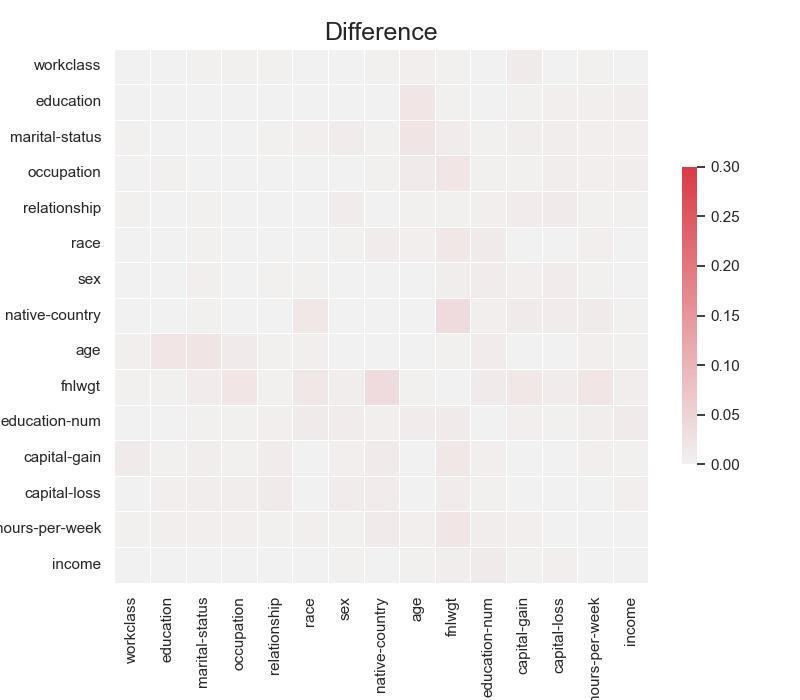
\includegraphics[width=\textwidth]{images/correlation_difference/real.jpg}
		\caption{Real}

	\end{subfigure}
	\hfill
	\begin{subfigure}{0.3\textwidth}
		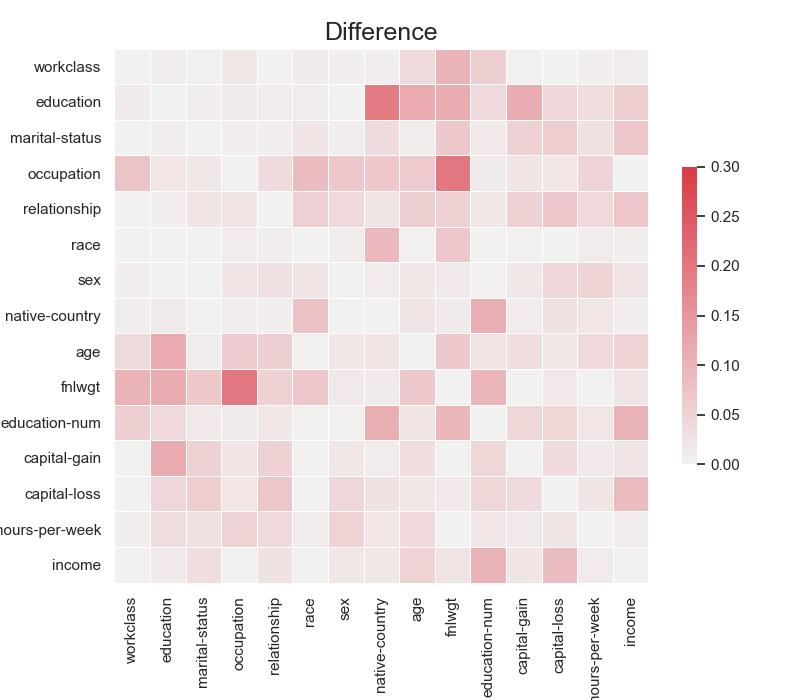
\includegraphics[width=\textwidth]{images/correlation_difference/tvae.jpg}
		\caption{TVAE$^{ml}$}

	\end{subfigure}
	\hfill
	\begin{subfigure}{0.3\textwidth}
		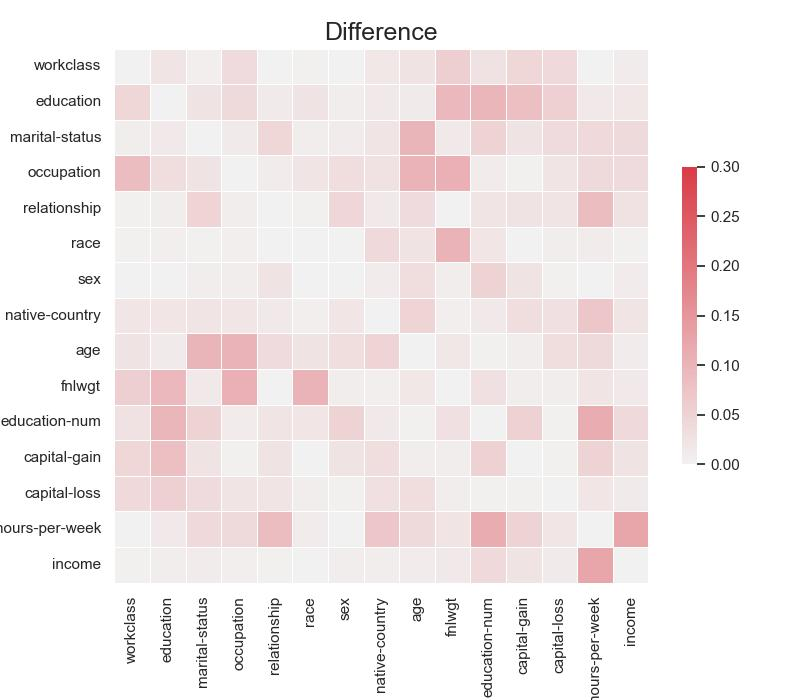
\includegraphics[width=\textwidth]{images/correlation_difference/ctabgan.jpg}
		\caption{CTABGAN$^{ml}$}
	\end{subfigure}

	\begin{subfigure}{0.3\textwidth}
		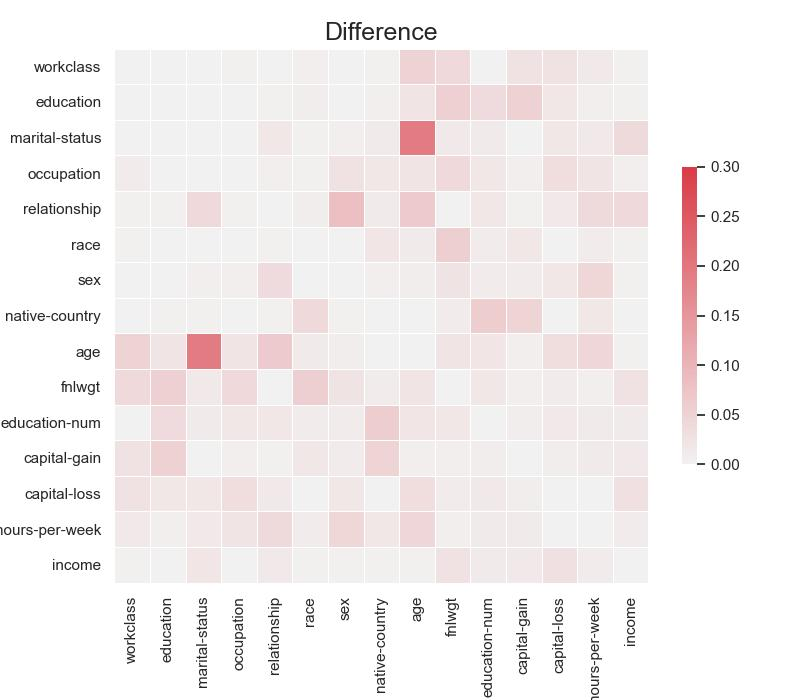
\includegraphics[width=\textwidth]{images/correlation_difference/ctabgan+.jpg}
		\caption{CTABGAN+$^{ml}$}

	\end{subfigure}
	\begin{subfigure}{0.3\textwidth}
		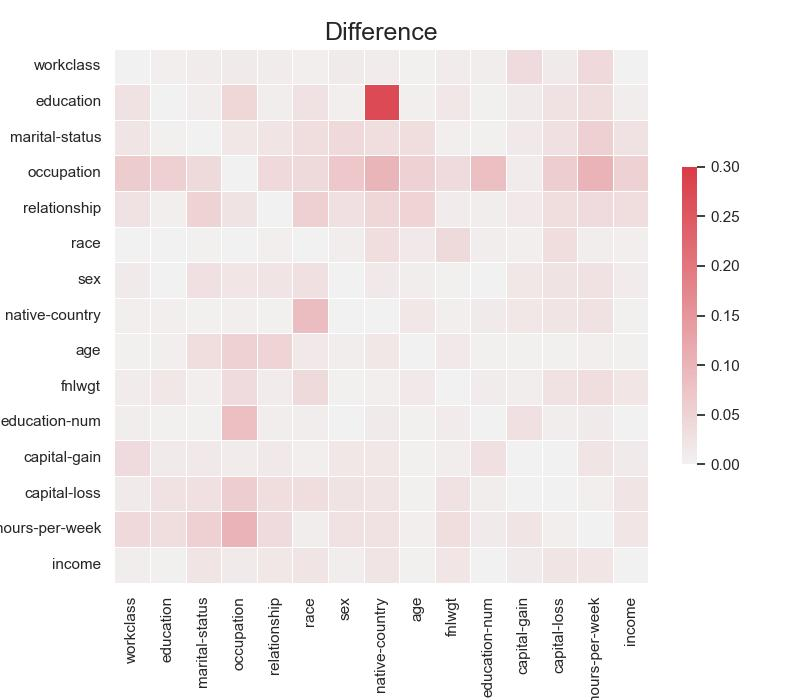
\includegraphics[width=\textwidth]{images/correlation_difference/smote.jpg}
		\caption{SMOTE}

	\end{subfigure}
	\begin{subfigure}{0.3\textwidth}
		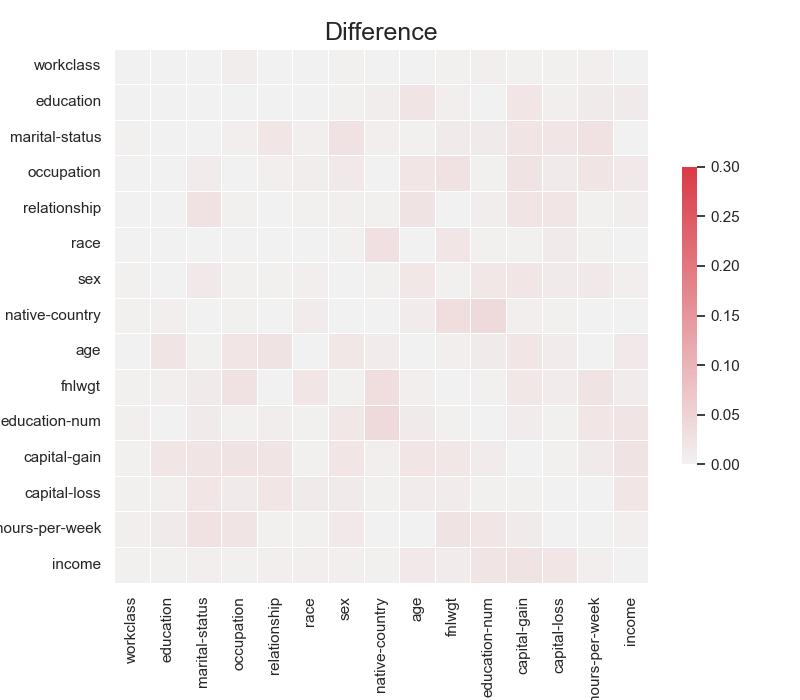
\includegraphics[width=\textwidth]{images/correlation_difference/tab-ddpm.jpg}
		\caption{TabDDPM$^{ml}_q$}
	\end{subfigure}
	\caption[Correlation plots Baseline Models]{Correlation Matrix difference for Baseline models.}
	\label{fig:corr_base}
\end{figure}


\begin{figure}[h]
	\begin{subfigure}{0.3\textwidth}
		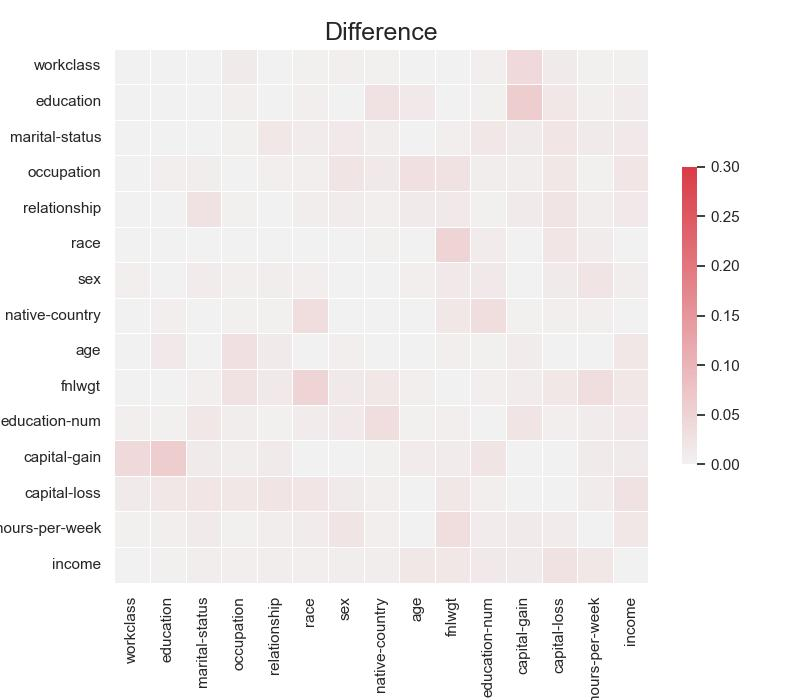
\includegraphics[width=\textwidth]{images/correlation_difference/tab-ddpm-bgm.jpg}
		\caption{TabDDPM-BGM$^{ml}_q$}
	\end{subfigure}
	\hfill
	\begin{subfigure}{0.3\textwidth}
		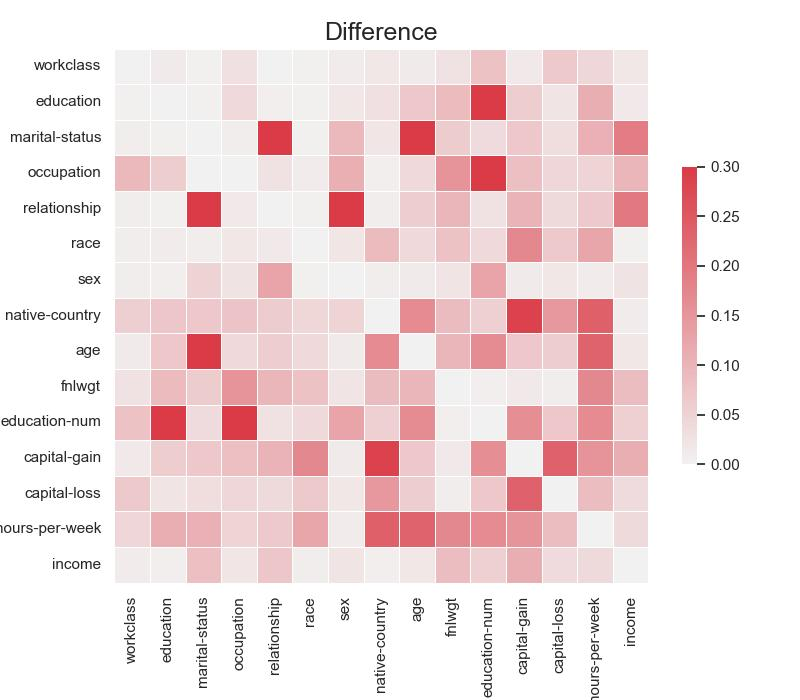
\includegraphics[width=\textwidth]{images/correlation_difference/tab-ddpm-ft.jpg}
		\caption{TabDDPM-FT$^{ml}_q$}
	\end{subfigure}
	\hfill
	\begin{subfigure}{0.3\textwidth}
		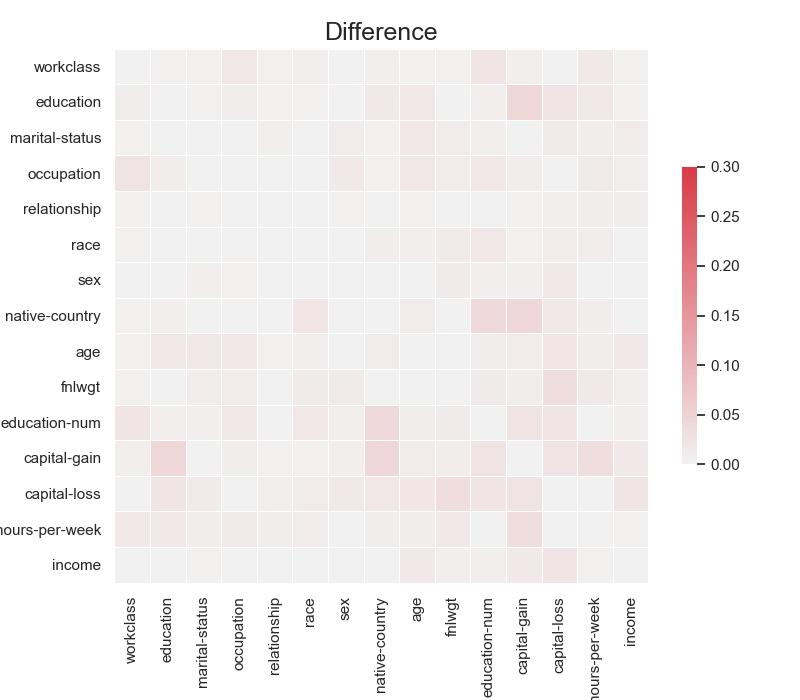
\includegraphics[width=\textwidth]{images/correlation_difference/tab-ddpm-bgm-simTune-minmax.jpg}
		\caption{TabDDPM-BGM$^{s}_m$}
	\end{subfigure}
	\caption[Correlation plots Experiment Models]{Correlation Matrix difference from selected experiment models.}
	\label{fig:corr_diffusion}
\end{figure}



\Autoref{fig:corr_diffusion} shows that while the TabDDPM-BGM$^{ml}$ are able to produce small correlation differences, the TabDDPM-FT$^{ml}$ is not able to reproduce
the correlation matrix of the real dataset.
The overall best correlation difference matrix is produced by TabDDPM$^{s}_m$, which is also reflected in their TabSynDex correlation score in \Autoref{tab:exp3-sim}, which is the highest across all \gls{model} versions.
Other \gls{model} version matrices do not show any noteworthy changes and are displayed in \Autoref{fig_a:corr_diff}.

\subsection{Principle Component Analysis}
\label{ch:results-pca}

A \gls{pca} is a dimensionality reduction technique that converts a dataset onto principal components \cite{brenninkmeijer2019GenerationEvaluationTabular}.
The components are then sorted according to the amount of variance from the original dataset each component is able to capture.
The following visualizations map the first two principal components, \ie the components that capture the most variance from data.


\begin{figure}[H]
	\centering
	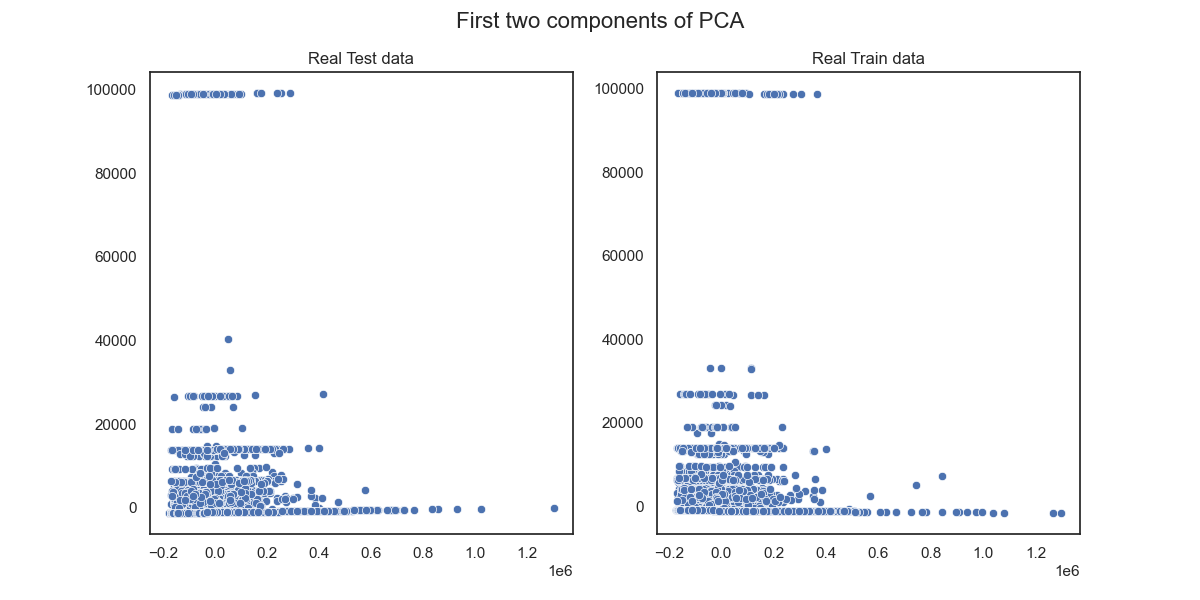
\includegraphics[width=0.7\textwidth]{images/pca/pca.png}
	\caption[PCA plot Real Data]{\gls{pca} for the real training and testing dataset}
	\label{fig:pca}
\end{figure}


\Autoref{fig:pca} shows the two \gls{pca} plots of the first two principal components from the real training and testing dataset.
One can see that the majority of values in the plots are scattered around the lower left corner (for $y<=40000$) with two accumulations of values spreading along the $x$-axis around $y=100000$ and $y=0$.
The goal of the synthetic data generation method is to produce synthetic data whose \gls{pca} plot is similar to the \gls{pca} plot of the real testing dataset.\newpage


\begin{figure}[H]
	\centering
	\begin{subfigure}{0.3\textwidth}
		\centering
		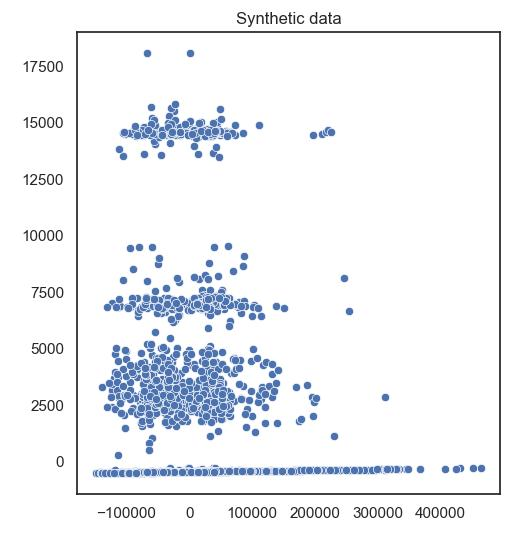
\includegraphics[width=\textwidth]{images/pca/tvae.jpg}
		\caption{TVAE$^{ml}$}
	\end{subfigure}
	\begin{subfigure}{0.3\textwidth}
		\centering
		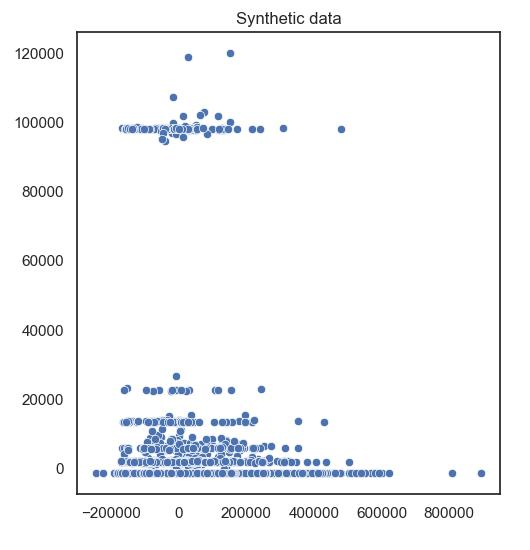
\includegraphics[width=\textwidth]{images/pca/ctabgan.jpg}
		\caption{CTABGAN$^{ml}$}
	\end{subfigure}
	\begin{subfigure}{0.3\textwidth}
		\centering
		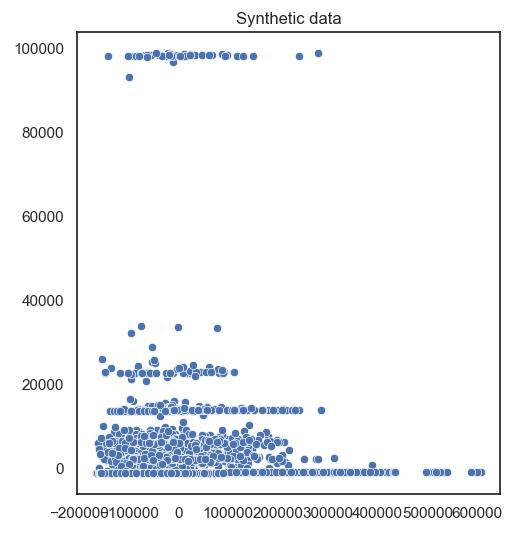
\includegraphics[width=\textwidth]{images/pca/ctabgan+.jpg}
		\caption{CTABGAN+$^{ml}$}
	\end{subfigure}
	\begin{subfigure}{0.3\textwidth}
		\centering
		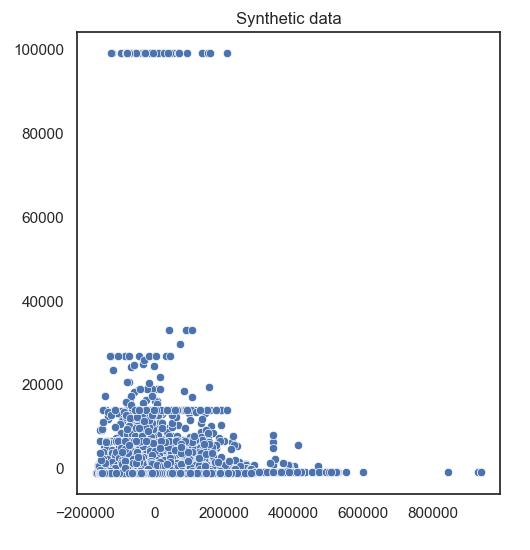
\includegraphics[width=\textwidth]{images/pca/smote.jpg}
		\caption{SMOTE}
	\end{subfigure}
	\begin{subfigure}{0.3\textwidth}
		\centering
		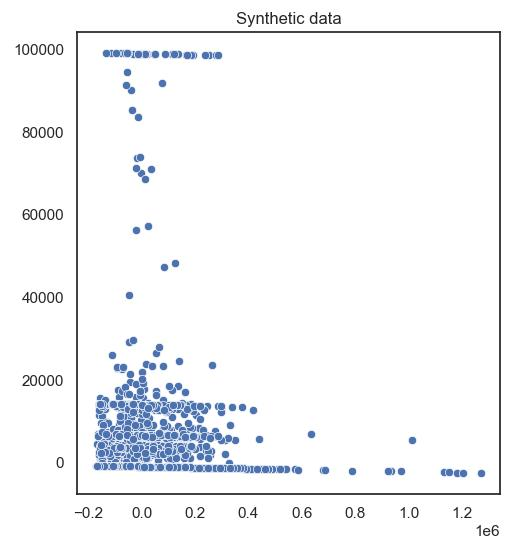
\includegraphics[width=\textwidth]{images/pca/tab-ddpm.jpg}
		\caption{TabDDPM$^{ml}_q$}
	\end{subfigure}
	\caption[PCA plots Baseline Models]{\gls{pca} for Baseline models.}
	\label{fig:pca_base}
\end{figure}


\begin{figure}[H]
	\centering
	\begin{subfigure}{0.3\textwidth}
		\centering
		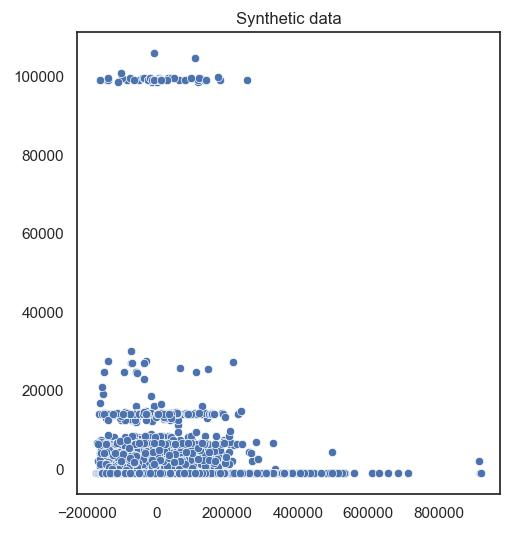
\includegraphics[width=\textwidth]{images/pca/tab-ddpm-bgm.jpg}
		\caption{TabDDPM-BGM$^{ml}_q$}
	\end{subfigure}
	\begin{subfigure}{0.3\textwidth}
		\centering
		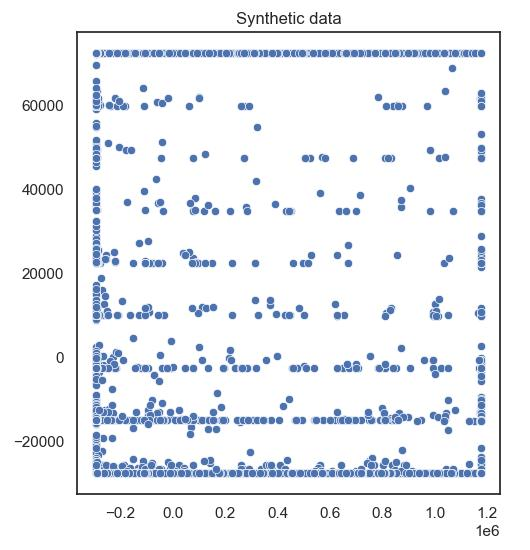
\includegraphics[width=\textwidth]{images/pca/tab-ddpm-ft.jpg}
		\caption{TabDDPM-FT$^{ml}_q$}
	\end{subfigure}


	\begin{subfigure}{0.3\textwidth}
		\centering
		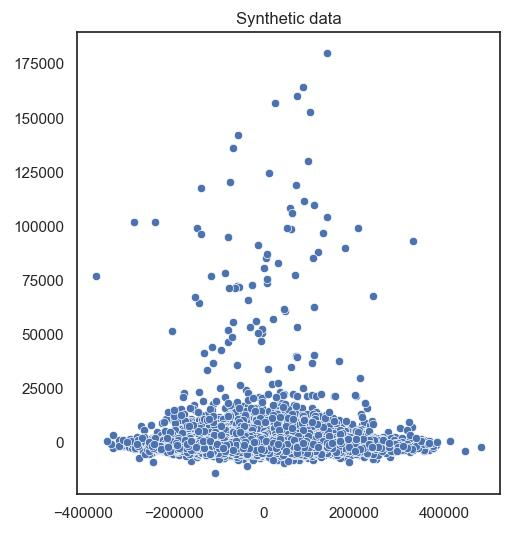
\includegraphics[width=\textwidth]{images/pca/tab-ddpm-simTune-minmax.jpg}
		\caption{TabDDPM$^{s}_m$}
	\end{subfigure}
	\begin{subfigure}{0.3\textwidth}
		\centering
		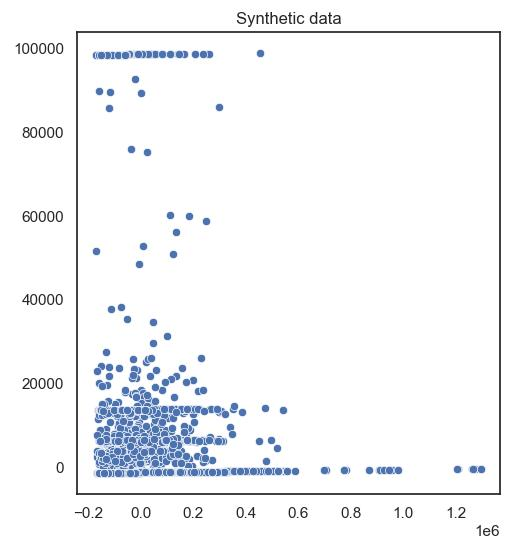
\includegraphics[width=\textwidth]{images/pca/tab-ddpm-simTune.jpg}
		\caption{TabDDPM$^{s}_q$}
	\end{subfigure}
	\caption[PCA plots Experiment Models]{\gls{pca} for selected experiment models.}
	\label{fig:pca_diffusion}
\end{figure}

\Autoref{fig:pca_base} shows the \gls{pca} plots for the different baseline models. 
All plots show some similarity with the \gls{pca}-plot from the original dataset, except for the TVAE \gls{model}. 
While it seems the CTABGAN, CTABGAN+, and TabDDPM models reproduce the main characteristics of the real \gls{pca} plot, they do have a few single outliers scattered.
These scatter outliers can be observed less frequently at the SMOTE \gls{pca} plot, which, out of the baseline models, recreates the original \gls{pca} plot the closest.


Out of the extended versions of TabDDPM, only the \gls{bgm} tabular processing mechanism seems to be able to produce a realistic \gls{pca}-plot (compare \Autoref{fig:pca_diffusion}).
Additionally, the min-max scaling seems to negatively affect the \gls{pca}-plot for the TabDDPM \gls{model}.
However, this did not occur for the TabDDPM-BGM \gls{model} that used min-max scaling (\Autoref{fig_a:pca_TabDDPMBM}).
This \gls{pca}-plot and the remaining \gls{model} versions plots can be found in Appendix \ref{A:pca}.

\subsection{Distribution Plot}
\label{ch:results-Distr}


For each \gls{model} version, distribution plots for each column can be found at Appendix \ref{A:distributions}, comparing the distributions of the synthetic data with the real data.
This section will highlight some interesting plots for selected models.

In terms of categorical distributions (\Autoref{fig:education} displays the education column distributions as an example), all baseline models can reproduce the original distributions,
with CTABGAN+$^{ml}$ and TabDDPM$^{ml}_q$ replicating the original distribution best.
The \gls{bgm} tabular processing \gls{model} also reproduced the categorical distributions in a comparable way to the TabDDPM counterpart.
On the other hand, the \gls{ft} tabular processing \gls{model} could not reproduce the original distribution at all and failed to mimic the real data.

Changing the hyperparameter tuning toward the similarity score did not affect the categorical distributions in any \gls{model}.
The same is valid for changing to the min-max scaling since it only affects continuous values.
\Autoref{fig:age} shows that this observation does not extend towards continuous columns, given the column age as an example.
Across the baseline models, CTABGAN+$^{ml}$ and TabDDPM$^{ml}_q$ are again best able to reproduce the original data distribution of the example column.
All TabDDPM-BGM models produce distributions that are comparable to those produced by the baseline TabDDPM.
Again, TabDDPM-FT fails to replicate the target distributions at all.
Interestingly, the similarity score hyperparameter optimization did not affect the TabDDPM distributions to any visible extent.
However, the Minmax scaling reduced the TabDDPM capability to create a realistic distribution, whose probability distributions rather follows a Gaussian distribution, failing to replicate the detailed peaks of the original dataset.
This behavior was not present in the \gls{bgm} version with min-max scaling.

Comparing all \gls{bgm} versions reveals interesting observations about the effect of applying normalizations after the tabular processing mechanisms.
Having no transformation or min-max transformation results in similar plots that can capture the overall distribution but deviate in some cases quite a lot (in the area of x=17 to 28 years).\newpage

\begin{figure}[H]
	\centering
	\begin{subfigure}{0.3\textwidth}
		\centering
		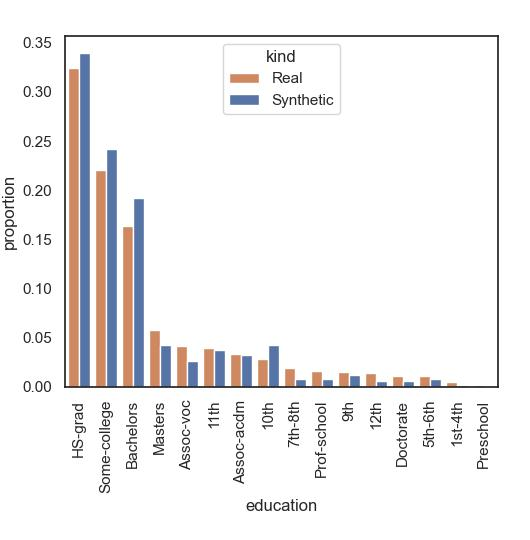
\includegraphics[width=\textwidth]{images/dist_education/tvae.jpg}
		\caption{TVAE$^{ml}$}
	\end{subfigure}
	\begin{subfigure}{0.3\textwidth}
		\centering
		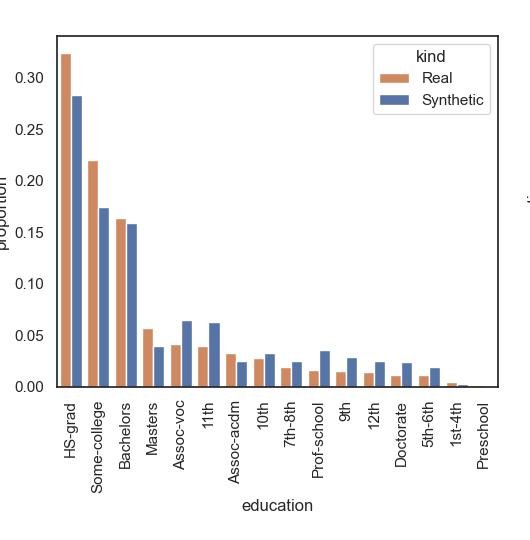
\includegraphics[width=\textwidth]{images/dist_education/ctabgan.jpg}
		\caption{CTABGAN$^{ml}$}
	\end{subfigure}
	\begin{subfigure}{0.3\textwidth}
		\centering
		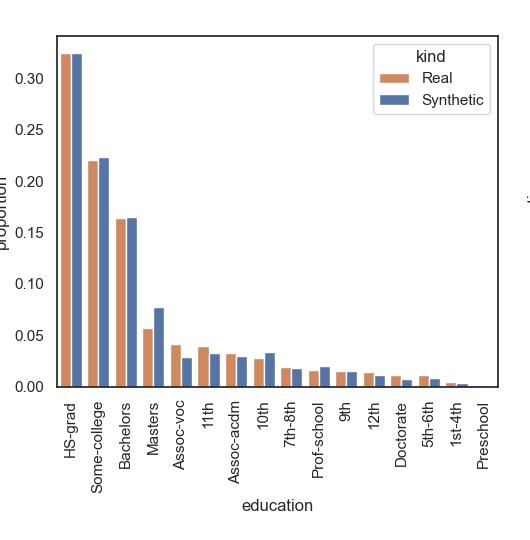
\includegraphics[width=\textwidth]{images/dist_education/ctabgan+.jpg}
		\caption{CTABGAN+$^{ml}$}
	\end{subfigure}


	\begin{subfigure}{0.3\textwidth}
		\centering
		\includegraphics[width=\textwidth]{images/dist_education/SMOTE.jpg}
		\caption{SMOTE}
	\end{subfigure}
	\begin{subfigure}{0.3\textwidth}
		\centering
		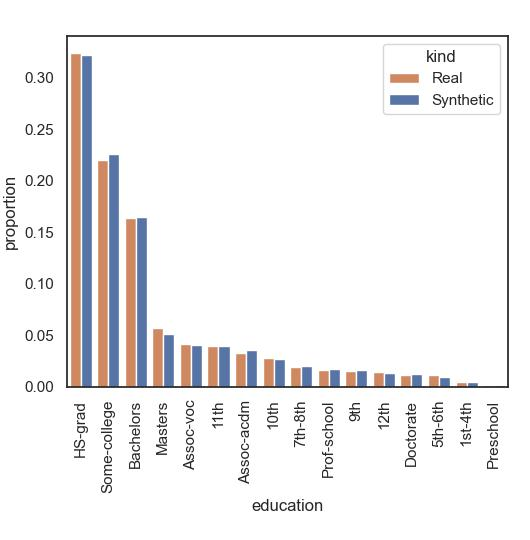
\includegraphics[width=\textwidth]{images/dist_education/tab-ddpm.jpg}
		\caption{TabDDPM$^{ml}_q$}
	\end{subfigure}  


	\begin{subfigure}{0.3\textwidth}
		\centering
		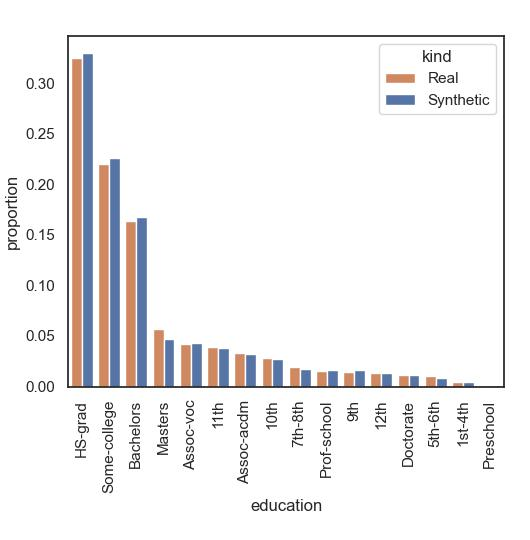
\includegraphics[width=\textwidth]{images/dist_education/tab-ddpm-bgm.jpg}
		\caption{TabDDPM-BGM$^{ml}_q$}
	\end{subfigure}
	\begin{subfigure}{0.3\textwidth}
		\centering
		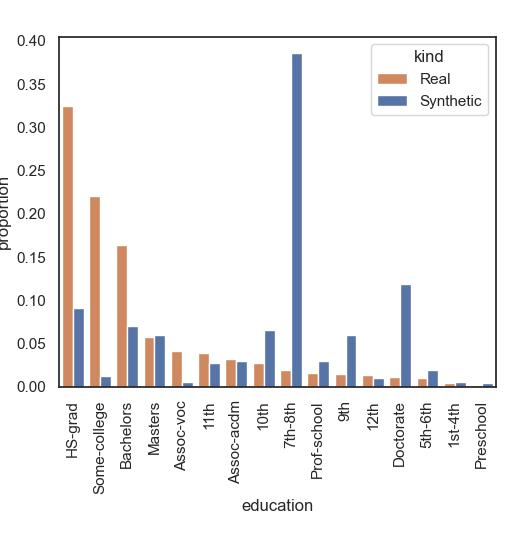
\includegraphics[width=\textwidth]{images/dist_education/tab-ddpm-ft.jpg}
		\caption{TabDDPM-FT$^{ml}_q$}
	\end{subfigure}
	\caption[Distribution Plots Categorical]{\textit{Education} column for baseline models.}
	\label{fig:education}
\end{figure}

Quantile transformation (TabDDPM-BGM$^{s}_q$) reduces the difference in this area, but an oversampling of entries with an age of 90 occurred.
Interestingly, out of all \gls{bgm} variations, the \gls{model} tuned after the machine learning efficacy (TabDDPM-BGM$^{ml}_q$) was best able to capture the distribution.
Looking at its \textit{age} distribution plot, it can be observed that big differences from the real data are few.
Nevertheless, undersampling of certain ages is present in the synthetic data.
However, one can observe that this is usually compensated with an oversampling of an age value close to it
(\eg undersampling of age x=17-18 is compensated by an oversampling of age x=19-20).\newpage


\begin{figure}[H]
	\centering
	\begin{subfigure}{0.3\textwidth}
		\centering
		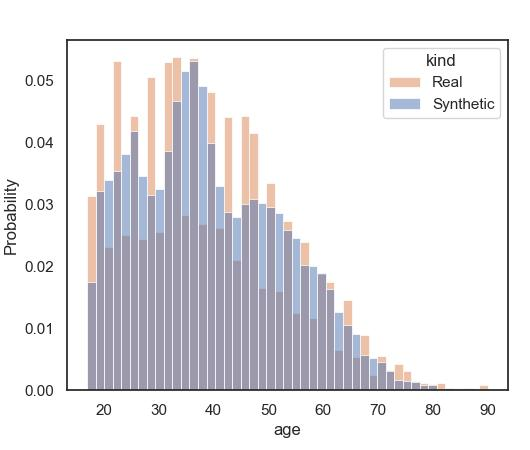
\includegraphics[width=\textwidth]{images/dist_age/tvae.jpg}
		\caption{TVAE$^{ml}$}
	\end{subfigure}
	\begin{subfigure}{0.3\textwidth}
		\centering
		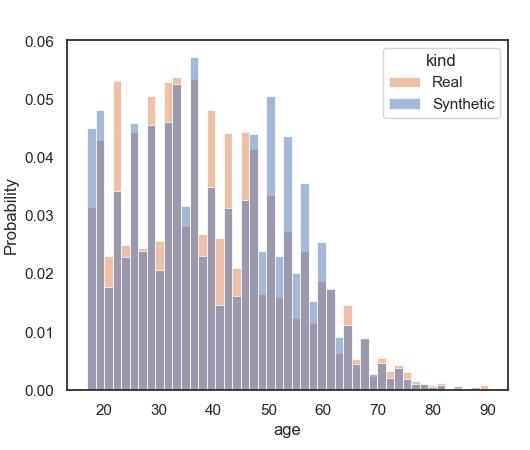
\includegraphics[width=\textwidth]{images/dist_age/ctabgan.jpg}
		\caption{CTABGAN$^{ml}$}
	\end{subfigure}
	\begin{subfigure}{0.3\textwidth}
		\centering
		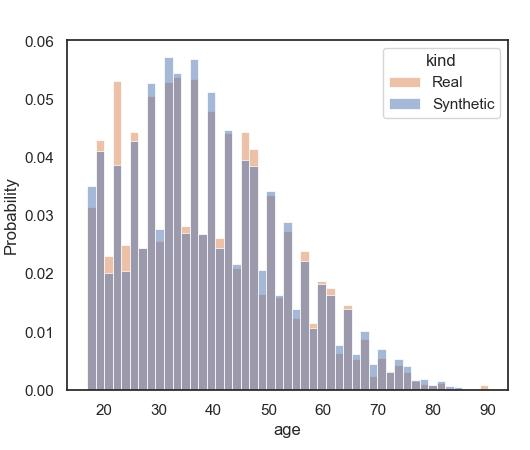
\includegraphics[width=\textwidth]{images/dist_age/ctabgan+.jpg}
		\caption{CTABGAN+$^{ml}$}
	\end{subfigure}


	\begin{subfigure}{0.3\textwidth}
		\centering
		\includegraphics[width=\textwidth]{images/dist_age/SMOTE.jpg}
		\caption{SMOTE}
	\end{subfigure}
	\begin{subfigure}{0.3\textwidth}
		\centering
		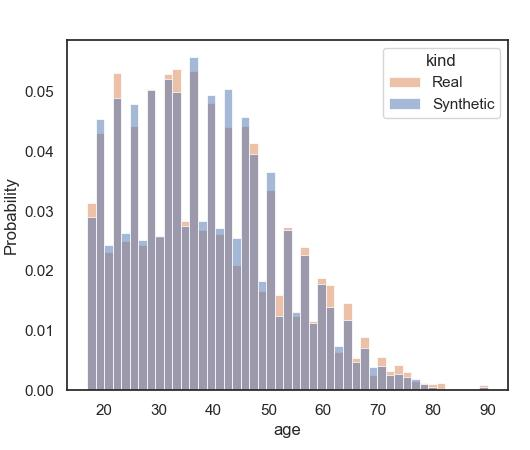
\includegraphics[width=\textwidth]{images/dist_age/tab-ddpm.jpg}
		\caption{TabDDPM$^{ml}_q$}
	\end{subfigure}
	\begin{subfigure}{0.3\textwidth}
		\centering
		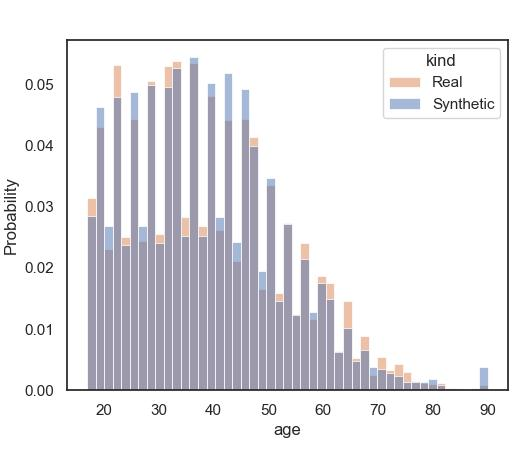
\includegraphics[width=\textwidth]{images/dist_age/tab-ddpm-simTune.jpg}
		\caption{TabDDPM$^{s}_q$}
	\end{subfigure}


	\begin{subfigure}{0.3\textwidth}
		\centering
		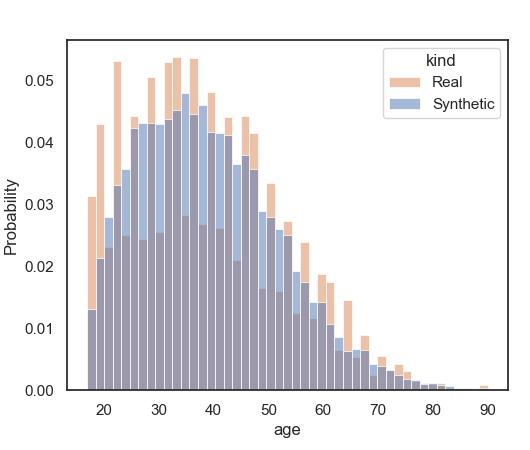
\includegraphics[width=\textwidth]{images/dist_age/tab-ddpm-simTune-minmax.jpg}
		\caption{TabDDPM$^{s}_m$}
	\end{subfigure}
	\begin{subfigure}{0.3\textwidth}
		\centering
		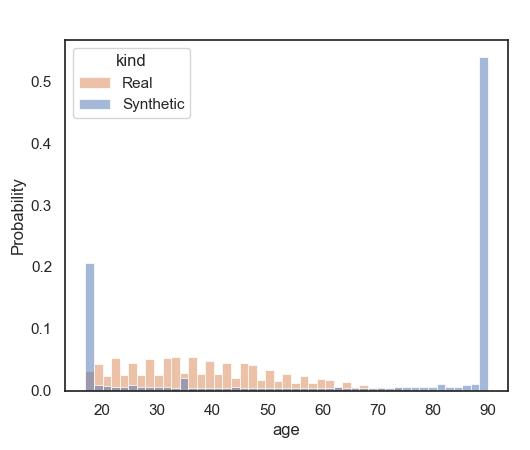
\includegraphics[width=\textwidth]{images/dist_age/tab-ddpm-ft.jpg}
		\caption{TabDDPM-FT$^{ml}_q$}
	\end{subfigure}
	\begin{subfigure}{0.3\textwidth}
		\centering
		\includegraphics[width=\textwidth]{images/dist_age/tab-ddpm-bgm.jpg}
		\caption{TabDDPM-BGM$^{ml}_q$}
	\end{subfigure}


	\begin{subfigure}{0.3\textwidth}
		\centering
		\includegraphics[width=\textwidth]{images/dist_age/tab-ddpm-bgm-simTune.jpg}
		\caption{TabDDPM-BGM$^{s}_q$}
	\end{subfigure}
	\begin{subfigure}{0.3\textwidth}
		\centering
		\includegraphics[width=\textwidth]{images/dist_age/tab-ddpm-bgm-simTune-minmax.jpg}
		\caption{TabDDPM-BGM$^{s}_m$}
	\end{subfigure}
	\begin{subfigure}{0.3\textwidth}
		\centering
		\includegraphics[width=\textwidth]{images/dist_age/tab-ddpm-bgm-simTune-none.jpg}
		\caption{TabDDPM-BGM$^{s}_n$}
	\end{subfigure}
	\caption[Distribution Plots Continuous]{\textit{Age} column for selected \gls{model} versions. Please note that the Y-axis range may vary due to the range of the synthetic data.}
	\label{fig:age}
\end{figure}
\newpage


\subsection{Cumulative Distribution Function}

\begin{figure}[H]
	\centering
	\begin{subfigure}{0.3\textwidth}
		\centering
		\includegraphics[width=\textwidth]{images/cdf/tvae.jpg}
		\caption{TVAE$^{ml}$}
	\end{subfigure}
	\begin{subfigure}{0.3\textwidth}
		\centering
		\includegraphics[width=\textwidth]{images/cdf/ctabgan+.jpg}
		\caption{CTABGAN+$^{ml}$}
	\end{subfigure}
	\begin{subfigure}{0.3\textwidth}
		\centering
		\includegraphics[width=\textwidth]{images/cdf/tab-ddpm-bgm.jpg}
		\caption{TabDDPM-BGM$^{ml}_q$}
	\end{subfigure}


	\begin{subfigure}{0.3\textwidth}
		\centering
		\includegraphics[width=\textwidth]{images/cdf/tab-ddpm-bgm-simTune.jpg}
		\caption{TabDDPM-BGM$^{s}_q$}
	\end{subfigure}
	\begin{subfigure}{0.3\textwidth}
		\centering
		\includegraphics[width=\textwidth]{images/cdf/tab-ddpm-ft.jpg}
		\caption{TabDDPM-FT$^{ml}_q$}
	\end{subfigure}
	\begin{subfigure}{0.3\textwidth}
		\centering
		\includegraphics[width=\textwidth]{images/cdf/tab-ddpm.jpg}
		\caption{TabDDPM$^{ml}_q$}
	\end{subfigure}


	\begin{subfigure}{0.3\textwidth}
		\centering
		\includegraphics[width=\textwidth]{images/cdf/tab-ddpm-simTune-minmax.jpg}
		\caption{TabDDPM$^{s}_m$}
	\end{subfigure}
	\begin{subfigure}{0.3\textwidth}
		\centering
		\includegraphics[width=\textwidth]{images/cdf/tab-ddpm-bgm-simTune-minmax.jpg}
		\caption{TabDDPM-BGM$^{s}_m$}
	\end{subfigure}
	\caption[CDF native-country]{\gls{cdf} plots for selected model versions for categorical the column "native-country" of the adult income dataset \cite{Dua:2019}}
	\label{fig:cdf}
\end{figure}

All \gls{cdf} plots can be found in Appendix \ref{A:cumsum}.
The plots show that the \glspl{cdf} of the synthetic data created by CTABGAN+$^{ml}$ and TabDDPM$^{ml}_q$ come closest to
the \glspl{cdf} of the real data across the baseline models (best visible for columns \textit{native-country} or \textit{hours-per-week}, compare \Autoref{fig:cdf, fig:cdf_hpw}).
The selected plots in \Autoref{fig:cdf, fig:cdf_hpw} show how the \gls{ft} tabular processing failed again to reproduce the original datas \gls{cdf}.
TabDDPM-BGM, on the other hand, produced synthetic data, whose \gls{cdf} correctly mimics the \gls{cdf} of the real data.
One could argue that TabDDPM and TabDDPM-BGM that have been tuned after the similarity score are slightly better able to
reproduce \gls{cdf} plots for categorical columns whose categories are imbalanced (\eg see column \textit{native-country}, where the majority of values equal \textit{United-States}).
This improvement is more prominent for the \gls{bgm} version.
The min-max scaling greatly affected the TabDDPM version and "smoothed out" its \glspl{cdf}.
This phenomenon was not present in the TabDDPM-BGM version with Minmax scaling.

\begin{figure}[H]
	\centering
	\begin{subfigure}{0.3\textwidth}
		\centering
		\includegraphics[width=\textwidth]{images/cdf_hpw/tvae.jpg}
		\caption{TVAE$^{ml}$}
	\end{subfigure}
	\begin{subfigure}{0.3\textwidth}
		\centering
		\includegraphics[width=\textwidth]{images/cdf_hpw/ctabgan+.jpg}
		\caption{CTABGAN+$^{ml}$}
	\end{subfigure}
	\begin{subfigure}{0.3\textwidth}
		\centering
		\includegraphics[width=\textwidth]{images/cdf_hpw/tab-ddpm-bgm.jpg}
		\caption{TabDDPM-BGM$^{ml}_q$}
	\end{subfigure}


	\begin{subfigure}{0.3\textwidth}
		\centering
		\includegraphics[width=\textwidth]{images/cdf_hpw/tab-ddpm-bgm-simTune.jpg}
		\caption{TabDDPM-BGM$^{s}_q$}
	\end{subfigure}
	\begin{subfigure}{0.3\textwidth}
		\centering
		\includegraphics[width=\textwidth]{images/cdf_hpw/tab-ddpm-ft.jpg}
		\caption{TabDDPM-FT$^{ml}_q$}
	\end{subfigure}
	\begin{subfigure}{0.3\textwidth}
		\centering
		\includegraphics[width=\textwidth]{images/cdf_hpw/tab-ddpm.jpg}
		\caption{TabDDPM$^{ml}_q$}
	\end{subfigure}


	\begin{subfigure}{0.3\textwidth}
		\centering
		\includegraphics[width=\textwidth]{images/cdf_hpw/tab-ddpm-simTune-minmax.jpg}
		\caption{TabDDPM$^{s}_m$}
	\end{subfigure}
	\begin{subfigure}{0.3\textwidth}
		\centering
		\includegraphics[width=\textwidth]{images/cdf_hpw/tab-ddpm-bgm-simTune-minmax.jpg}
		\caption{TabDDPM-BGM$^{s}_m$}
	\end{subfigure}
	\caption[CDF hours-per-week]{\gls{cdf} plots for selected model versions for the numerical column "hours-per-week" of the adult income dataset \cite{Dua:2019}}
	\label{fig:cdf_hpw}
\end{figure}




%CF Hours_per_week




\newpage
\section{Discussion}
\label{ch:results-discussion}
The goal of this thesis was to investigate the performance of adding the tabular processing mechanisms to the TabDDPM \gls{model} (\gls{rq}1) and
to expand upon the already existing machine learning efficacy evaluation performed by \cite{kotelnikov2022TabDDPMModellingTabular} through the similarity score metrics proposed by \cite{chundawat2022UniversalMetricRobust}.

\subsection*{Analysis of Visual and Numerical Results}

\begin{table}[h]
	\centering
	\begin{tabular}{lrrr}
		\toprule
		\textbf{Model}        & \textbf{Accuracy} & \textbf{F1}    & \textbf{ROC-AUC} \\
		\midrule
		Real                  & 0.874              & 0.815          & 0.928            \\
		TVAE$^{ml}$           & 0.845              & 0.780          & 0.900            \\
		SMOTE                 & 0.858              & 0.791          & 0.910            \\
		CTABGAN$^{ml}$        & 0.850              & 0.775          & 0.900            \\
		CTABGAN+$^{ml}$       & 0.855              & 0.775          & 0.907            \\
		TabDDPM$^{ml}_q$      & 0.860              & 0.794          & 0.913            \\
		TabDDPM-BGM$^{ml}_q$  & \textbf{0.863}     & \textbf{0.798} & \textbf{0.916}   \\
		TabDDPM-FT$^{ml}_q$   & 0.785              & 0.552          & 0.821            \\
		CTABGAN$^{s}_q$       & 0.850              & 0.776          & 0.900            \\
		CTABGAN+$^{s}$        & 0.851              & 0.768          & 0.902            \\
		TVAE$^{s}$            & 0.845              & 0.780          & 0.900            \\
		TabDDPM$^{s}_q$       & 0.856              & 0.782          & 0.908            \\
		TabDDPM-BGM$^{s}_q$   & 0.859              & 0.792          & 0.911            \\
		TabDDPM-FT$^{s}_q$    & 0.766              & 0.451          & 0.712            \\
		TabDDPM$^{s}_m$       & 0.856              & 0.778          & 0.910            \\
		TabDDPM-BGM$^{s}_m$   & 0.857              & 0.787          & 0.909            \\
		TabDDPM-BGM$^{s}_{n}$ & 0.855              & 0.784          & 0.907            \\
		\bottomrule
		\multicolumn{4}{c}{}\\[-0.6em]
	\end{tabular}
	\caption[Overview all ML-Efficacy results]{Overview of all CatBoost machine learning efficacy results for all tested model versions.}
	\label{tab:ml-all}
\end{table}


\begin{table}[h]
	\centering
	\begin{tabular}{lrrrrrr}
		\toprule
		\textbf{Model}        & \textbf{Similarity Score} & \textbf{Basic} & \textbf{Correlation} & \textbf{ML}    & \textbf{Support} & \textbf{pMSE}  \\
		\midrule
		Real                  & 0.960                     & 0.992          & 0.943                & 0.998          & 0.984            & 0.882          \\
		TVAE$^{ml}$           & 0.658                     & 0.854          & 0.814                & 0.962          & 0.657            & 0.000          \\
		SMOTE                 & 0.723                     & 0.953          & 0.865                & 0.992          & 0.804            & 0.000          \\
		CTABGAN$^{ml}$        & 0.741                     & 0.940          & 0.832                & 0.984          & 0.947            & 0.000          \\
		CTABGAN+$^{ml}$       & 0.750                     & 0.969          & 0.882                & 0.990          & 0.892            & 0.019          \\
		TabDDPM$^{ml}_q$      & 0.759                     & 0.973          & 0.919                & 0.992          & 0.874            & 0.035          \\
		TabDDPM-BGM$^{ml}_q$  & 0.742                     & 0.964          & 0.918                & \textbf{0.996} & 0.831            & 0.000          \\
		TabDDPM-FT$^{ml}_q$   & 0.595                     & 0.495          & 0.648                & 0.869          & 0.963            & 0.000          \\
		CTABGAN$^{s}$         & 0.740                     & 0.938          & 0.833                & 0.984          & 0.947            & 0.000          \\
		CTABGAN+$^{s}$        & 0.784                     & 0.970          & 0.888                & 0.987          & 0.908            & 0.167          \\
		TVAE$^{s}$            & 0.658                     & 0.856          & 0.815                & 0.962          & 0.656            & 0.000          \\
		TabDDPM$^{s}_q$       & 0.852                     & 0.976          & 0.921                & 0.991          & 0.952            & 0.420          \\
		TabDDPM-BGM$^{s}_q$   & 0.857                     & \textbf{0.982} & 0.858                & 0.991          & 0.920            & 0.532          \\
		TabDDPM-FT$^{s}_q$    & 0.588                     & 0.512          & 0.619                & 0.818          & \textbf{0.992}   & 0.000          \\
		TabDDPM$^{s}_m$       & \textbf{0.869}            & 0.938          & \textbf{0.930}       & 0.990          & 0.928            & \textbf{0.558} \\
		TabDDPM-BGM$^{s}_m$   & 0.856                     & 0.981          & 0.913                & 0.992          & 0.915            & 0.476          \\
		TabDDPM-BGM$^{s}_{n}$ & 0.833                     & 0.975          & 0.916                & 0.992          & 0.915            & 0.369          \\
		\bottomrule
		\multicolumn{7}{c}{}\\[-0.6em]
	\end{tabular}
	\caption[Overview all TabSynDex results]{Overview of all TabSynDex score results for all tested model versions.}
	\label{tab:sim-all}
\end{table}


Based on the obtained results, it is evident that the processing mechanism for \gls{ft} has failed and is not advisable.
Despite having the highest overall support score, all other measurements and visual representations indicate that the \gls{model} could not generate synthetic data that closely resembles the original dataset.
The reason why the \gls{ft} processing does not work well even though it performed well in the cell imputation task \cite{zheng2022DiffusionModelsMissing} remains unclear.
As a consequence, the TabDDPM-FT variations will not be further discussed or analyzed.

The \gls{bgm} processor variant was able to produce not only good numerical but also visual results.
In terms of machine learning efficacy, the TabDDPM-BGM$^{ml}_q$ version shows the best machine learning efficacy performance across all tested metrics (\Autoref{tab:ml-all}: Accuracy, F1 and AUC-ROC and \Autoref{tab:sim-all}: ML).
However, the advantage over its simpler counterpart TabDDPM$^{ml}_q$ is only marginal (+0.003\%-points).
Overall, models with hyperparameters tuned towards machine learning efficacy outperform models with hyperparameters tuned towards similarity score in the machine learning efficacy scores, as one would expect.
The results of the non-diffusion baseline models show that the\gls{smote}approach is a reliable sampling technique when the synthetic data will be used in a machine-learning scenario.
Its machine learning efficacy results are superior to the other non-diffusion baseline models, while the \gls{model} is overall less complex.
For other scenarios, CTABGAN+ achieves the best overall performance in terms of numerical and visual results for non-diffusion-based models.
Nevertheless, the best-found CTABGAN+ version is inferior to the best-found diffusion \gls{model}.

Changing the tuning strategy to the similarity score allowed several observations to be made.
Firstly for the non-diffusion models', metric results had not significantly changed after switching to similarity score tuning.
All of their metric scores stayed roughly the same, with the exception of CTABGAN+.
Only for the this \gls{model}, a similarity tuning resulted in a noteworthy metric increase, especially for its \gls{pmse} score, which increased by +0.14\%-points.

Diffusion models, on the other hand, showed more noteworthy changes in their numerical metric results.
Overall, diffusion models with a similarity score tuning show reduced machine learning efficacy metric scores compared to their machine learning efficacy counterparts.
While this reduction is relatively small, the similarity metrics have increased significantly.
Specifically, through the adjustment of the hyperparameters towards the similarity score, which includes the PMSE score, an increase in the \gls{pmse} score was notably achieved.
Especially for diffusion models, this big increase in the \gls{pmse} score is worth highlighting.
For Models such as TabDDPM and TabDDPM-BGM, this similarity tuning resulted in \gls{pmse} values increasing to a score between $0.42$ and $0.55$.
The same tuning strategy did not affect the \gls{pmse} score of baseline models like TVAE or CTABGAN; only CTABGAN+ was affected but at a lower amplitude compared to diffusion models.
These\ gls{pmse} scores indicate, that almost all non-diffusion baseline models failed to produce data that is non-differentiable from the real data by a logistic regression \gls{model}.
This finding aligns with the observation made by \textcite{chundawat2022UniversalMetricRobust}, who also observe that all of their tested models (mainly \gls{gan}-based) achieve a \gls{pmse} of 0.
The experiments of \textcite{chundawat2022UniversalMetricRobust} only identified one \gls{model}, a \gls{gan} \gls{model} with gradient penalty and Wasserstein distance, which was able to achieve a peak \gls{pmse} score of $0.4$ (scores are not comparable, since a different dataset was used).
Overall, this indicates that diffusion-based models are better able to produce synthetic data that is harder to differentiate from its real counterpart.

In addition to the increase of the \gls{pmse} score, the other metrics that make up the similarity score have also increased, but on a smaller scale.
Only correlation values got decreased slightly through the similarity tuning.
This observation holds for TabDDPM and TabDDPM-BGM but not for the baseline models (TVAE and CTABGAN), whose metric results remained unchanged after switching the tuning strategy.
This indicates that the importance of hyperparameter tuning is much higher for diffusion models in tabular data synthesis, as their tuning strategy affects the metric outcomes significantly.

Replacing the quantile transform function with min-max scaling for the TabDDPM (TabDDPM$^{s}_m$) has led to the highest overall similarity score.
It scored highest in both correlation and \gls{pmse}, leading to a high overall similarity score.
According to \cite{scikit-learndevelopers2023QuantileTransformer}, the quantile transform function is a non-linear transformation that may distort correlations between variables.
This is also observable in the correlation metric score, where TabDDPM$^{s}_q$ and TabDDPM-BGM$^{s}_q$ have a lower correlation score than their min-max scaling counterpart.
However, it is essential to also take into consideration the visual results.
Although the correlation difference plot of TabDDPM$^{s}_m$ appears satisfactory, the distribution and \gls{cdf} plot of continuous columns (compare \Autoref{fig_a:dist_3_c,fig_a:cumsum_3_c}) look worse when compared to those of other models.
The continuous plots of TabDDPM$^{s}_m$ lack details and rather approximate the original distribution.
The \gls{model}'s quantile transform counterpart TabDDPM$^{s}_q$ does not show this behavior, producing overall more realistic plots.
This indicates that the min-max scaling, which is applied to the numerical columns, causes this kind of behavior.
Since min-max scaling scales the data according to the minimum and maximum value with the column, it is susceptible to outliers.
This results in a bad normalization if even one value in the column is unusually large or small.
The \gls{bgm} processor also makes use of a form of min-max encoding in their "general transform" \cite[p. 7]{zhao2022CTABGANEnhancingTabular} (compare \Autoref{ch:BGMProcessor}).
However, \textcite{zhao2022CTABGANEnhancingTabular} emphasizes as well that this encoding should only be applied to simple continuous distributions like a single-mode Gaussian distribution.
TabDDPM-BGM$^{s}_m$ does not show this behavior even though min-max scaling is applied.
A possible explanation for why the TabDDPM-BGM variants are not affected by a min-max scaling in the same way as TabDDPM is related to the mode-specific normalization.
Recall that mode-specific normalization transforms numerical columns into a vector consisting of an $\alpha$ and a $\beta$ part.
The $\alpha$ part is the normalized value according to the most likely mode, which is indicated in the \gls{oh} vector $\beta$.
The \textit{TabularProcessor} splits the $\alpha$ and $\beta$ parts up and assigns them to the numerical and categorical output arrays respectively.
This was required since the diffusion for numerical and categorical values is different (Gaussian diffusion for numerical and Multinomial diffusion for categorical).
Only after this, the normalization through min-max is applied (and only to the numerical values). 
But since all the $\alpha$ values are already normalized, the impact of an additional normalization through the min-max function is most likely reduced.

In summary, the following observations could be made:

\begin{itemize}
	\item The processing mechanism for \gls{ft} has failed and is not advisable, as it could not generate synthetic data that closely resembles the original dataset.
	\item The \gls{bgm} processor produced good numerical and visual results.
	\item TabDDPM-BGM$^{ml}_q$ shows the best machine learning efficacy performance across all tested models.
	\item Out of the baseline models,\gls{smote}is a reliable sampling technique for non-diffusion baseline models in machine learning scenarios.
	      In other scenarios, CTABGAN+$^{s}$ is the preferred non-diffusion \gls{model}.
	\item Diffusion models outperform non-diffusion models in tabular data synthesis.
	\item Diffusion models with similarity score tuning led to models with a non-zero \gls{pmse} score.
	\item Hyperparameter tuning is more important for diffusion models in tabular data synthesis than for non-diffusion models, as their tuning strategy significantly affects metric outcomes.
	\item Replacing the quantile transform function with min-max scaling for TabDDPM (TabDDPM$^{s}_m$) led to the highest overall similarity score but also resulted in worse distributions and \gls{cdf} plots of continuous columns.
	\item TabDDPM-BGM is not affected by quantile or min-max scaling to the same extent as the plain TabDDPM.
\end{itemize}
\newpage

\subsection*{Analysis of Research Questions}

\subsubsection{RQ1}

The results obtained in this study provide insights into the research questions posed in \Autoref{ch:intro-goals}.
\gls{rq}1 is concerned with the effects of additional tabular data processing mechanisms on TabDDPM.
By incorporating additional tabular data processing mechanisms, the TabDDPM \gls{model} improved performance compared to the baseline models.
However, this was only the case for the \gls{bgm} processing but not the \gls{ft} processing.
It was found that the TabDDPM-BGM$^{ml}_q$ is the best-suited \gls{model} for producing synthetic data that will be used in a machine-learning scenario.
For other scenarios, a TabDDPM-BGM variation tuned towards the similarity score should be preferred.
Even though TabDDPM$^{s}_m$ achieved the highest overall similarity score, its visual results lack detail for numerical columns.
Hence when using TabDDPM-BGM, TabDDPM-BGM$^{s}_q$ should be preferred when slightly better Basic, Support, and \gls{pmse} scores are desired and TabDDPM-BGM$^{s}_m$ when good correlations are of importance.

The visual results reinforced these findings, with correlation differences and \gls{pca} plots produced by TabDDPM-BGM variants closely resembling the original dataset.
In addition to that, TabDDPM-BGM versions are reliably able to reproduce distributions and \glspl{cdf} of the original dataset.
The most significant difference was observable when replacing the quantile transformation with the min-max scaling.
While the plain TabDDPM$^s_m$ \gls{model} struggled to reproduce the detail in the original continuous columns, the \gls{bgm} processing variant was able to.

To summarize, the tabular processor encodes the data into a different data format, which will be processed by the TabDDPM afterward.
Depending on the encoded data format, the generative capability of TabDDPM changed.
From the \gls{ft} processed data, the TabDDPM \gls{model} could not generate realistic synthetic data.
On the other hand, the \gls{bgm} technique encoded the data reliably, such that the diffusion \gls{model} could produce synthetic data that closely resembled the original dataset in multiple aspects.
With the \gls{bgm} technique, the TabDDPM showed slightly improved generative capabilities, better performance across various metrics, and more realistic synthetic data generation compared to TabDDPM without \gls{bgm}.
Hence, the results suggest that introducing a tabular processor to the synthesis pipeline can improve the overall quality of the produced synthetic data.
\newpage

\subsubsection{RQ2}
\gls{rq}2 is concerned with an extended evaluation of Diffusion based tabular data synthesis that goes beyond a machine learning efficacy evaluation.
In this thesis, the TabSynDex evaluation metric \cite{chundawat2022UniversalMetricRobust}, in addition to a CatBoost machine learning efficacy, was applied.
This evaluation revealed new insights into the performance of diffusion-based models compared to other \gls{model} types in tabular data synthesis.
Overall, it could be observed that the superior performance of TabDDPM compared to the non-diffusion models found in \cite{kotelnikov2022TabDDPMModellingTabular}
could not only be confirmed with the results of this thesis but it could be shown that the superior performance also extends to the other tested metrics (basic statistics, correlations, ml, support, \gls{pmse}).

Furthermore, the evaluation also highlights the importance of hyperparameter tuning for diffusion models in tabular data synthesis.
While a change in the hyperparameter tuning strategy hardly affected non-diffusion models, it greatly affected the TabDDPM approach.
If hyperparameters are tuned towards the TabSynDex Similarity score, diffusion models outperform all other models, including \gls{vae} and \gls{gan}-based approaches,
in all tested metrics.
The most significant effect was visible in the \gls{pmse} score, indicating the differentiability of the synthetic data from the real data.
Non-diffusion models consistently produced synthetic data that resulted in a near-zero \gls{pmse} score, even if their hyperparameters have been tuned to maximize it.
However, diffusion \gls{model} variants tested in this thesis were able to produce \gls{pmse} scores of up to 0.55\%.

The evaluation strategy in this thesis also included analysis of visualizations of the synthetic data in multiple ways.
This evaluation revealed that TabDDPM and its variances produce synthetic data whose plots resemble the original data plots more closely than the synthetic data plots of non-diffusion models.
Additionally, the visual inspection revealed the effects of changing the hyperparameter tuning strategy or data preprocessing strategy has on diffusion models.
For example, TabDDPM$^{s}_m$ metrics result suggest that it produces the best \gls{model} overall to produce synthetic data, as it has the highest overall similarity score.
However, its plots show a reduced capability to recreate continuous columns accurately.

In summary, the evaluation performed in the thesis showed that TabDDPM and its \gls{bgm} variant outperform other generative models,
including \gls{vae} and \gls{gan}-based approaches, in an extended similarity evaluation based on the TabSynDex metric,
machine learning efficacy, and a visualization analysis.
Hyperparameter tuning greatly affected the performance of diffusion models, and visualizations revealed that diffusion models produce synthetic data that more closely resemble the original data than non-diffusion models.
Ultimately, this thesis showed the importance of an elaborate evaluation of synthetic data, as new insights on the behavior of diffusion models for tabular data synthesis could be gained,
which are of benefit for the development of potential future diffusion-based models.
Additionally, such an extended evaluation allows for a holistic view of the produced synthetic data, uncovering strengths and weaknesses from different perspectives.
\newpage
\section{Limitations}
\label{ch:results-limitations}
%-------------------------------------------------------------------------

This study has some limitations that need to be acknowledged.
The most significant limitation is that only one real dataset (the adult dataset \cite{Dua:2019}) has been used to evaluate the performance of different models.
Therefore, it is possible that some \gls{model} versions may perform better or worse on other datasets with different characteristics such as size, dimensionality, or complexity.
The reason for this was the limited access to computing resources.
Consequently, all observations and results made in this thesis only hold for the adult dataset and should not be generalized until they can be confirmed on multiple datasets.

A second limitation is that only a fixed set of hyperparameters were tested during hyperparameter tuning.
Therefore, it is possible that some methods may benefit from further optimization or customization.

Furthermore, although the set of evaluation metrics has been larger compared to the original authors \cite{kotelnikov2022TabDDPMModellingTabular},
an additional, even more extensive evaluation should be considered.
In particular, this experiment did not consider privacy- and model-complexity-related metrics that would likely reveal new valuable insights.

Lastly, diffusion models, like most other deep neural networks, suffer from a lack of interpretability, as they are considered a black-box \gls{model} \cite{benitez1997AreArtificialNeural}.
\chapter{Conclusion and Future Work}
\label{ch:conclusion}

\section{Conclusion}
\label{ch:conclusion_}

This thesis investigates the effect of different tabular processing mechanisms on diffusion-based tabular data synthesis.
An already existing tabular data generation pipeline has been extended to implement different tabular encoding and decoding strategies easily.
The pipeline of TabDDPM \cite{kotelnikov2022TabDDPMModellingTabular} was extended by two tabular processing mechanisms that encode the tabular data before the training and revert the data back after sampling synthetic data.
The extended pipeline was evaluated using a CatBoost-based machine learning efficacy evaluation, a TabSynDex metric, and visualization of the synthetic data.
The TabSynDex metric comprises five sub-metrics that capture different similarity aspects of the synthetic data.
Several observations could be made in a set of experiments.
Firstly, the results in terms of machine learning efficacy stated by the authors of the TabDDPM pipeline could be reproduced \cite{kotelnikov2022TabDDPMModellingTabular}.
Thanks to the addition of the TabSynDex metrics, it has been shown that TabDDPM superior performance against a set of non-diffusion baseline models also extends to the TabSynDex similarity metrics.

Adding a \acrfull{ft} processing mechanism into the TabDDPM generation pipeline transforms the tabular data in such a way,
that the diffusion model was not able to generate any meaningful data, which could be seen in the visual result.
Adopting a more complex encoding/decoding strategy from \cite{zhao2022CTABGANEnhancingTabular}, which uses a \acrfull{bgm},
improved TabDDPM's generative capabilities in producing synthetic data that is useful in machine-learning scenarios.
Hence, it could be shown that changing the tabular data format greatly affects the diffusion model's generative capability, in a negative (for the \gls{ft} approach) and positive way (for the \gls{bgm} approach).

Furthermore, the importance of hyperparameter tuning for diffusion models was highlighted.
Diffusion models tuned towards the TabSynDex similarity score greatly improved several of the TabSynDex metrics.
In the performed experiments, diffusion models have been the first models to achieve a non-zero \gls{pmse} score, which other current state-of-art models have not been capable of.
Hence, diffusion models are better at producing synthetic data that is more non-differentiable from the real data \cite{chundawat2022UniversalMetricRobust} compared to tested non-diffusion models.
Further experiments showed how changing the data normalization strategy can, on the one hand, increase metric results but, on the other hand, worsen visual results.
This insight underlines the importance of a visual evaluation of synthetic data to estimate the quality of the produced synthetic data properly.
From all performed experiments, it can be concluded that diffusion-based tabular data synthesis is superior to the synthesis of other model types, such as \glspl{gan} or \glspl{vae}.
Moreover, diffusion models have not only shown overall better metric and visual results, but they are also more flexible, as a hyperparameter tuning already affects the outcome of the metrics greatly.
Even though TabDDPM$^{s}_{m}$ achieved the highest overall similarity score, it is not able to reproduce the underlying characteristics of the real data, which could be seen in the several of the comparative visualizations presented in this thesis.
TabDDPM$^{s}_{m}$ lacks the ability to properly recreate important characteristics of the real data, such as column distributions (\Autoref{fig:age}) or the real datasets principal components (\Autoref{fig:pca_diffusion}).
This was not the case for TabDDPM-BGM$^{s}_{[q|m]}$ models, which achieved only slightly worse similarity scores but better capture the underlying characteristics of the real data, as indicated by the visual plots in this thesis.
As a consequence, the TabDDPM-BGM$^{s}_{[q|m]}$ variants should be considered as the best overall models of this thesis.
Nevertheless, potential users should alter the model pipeline design depending on the use case of the synthetic data, since TabDDPM-BGM$^{s}_m$ produced the best correlation score, TabDDPM-BGM$^{ml}_q$ the best machine learning efficacy scores and TabDDPM-BGM$^{s}_q$ the best basic statistical values and \gls{pmse} results.
\newpage

\section{Future Work}
\label{ch:results-futureWork}

As implementing diffusion models for synthesizing tabular data represents a relatively innovative approach with limited research to date, numerous promising pathways for future investigations exist.
Firstly, to overcome the limitations presented in \Autoref{ch:results-limitations}, a more extensive set of datasets is required to confirm the results observed in this thesis.
More datasets with diverse characteristics to generalize the findings and identify potential sources of variation or bias.

Moreover, incorporating a variety of metrics with diverse perspectives is essential for evaluating the performance and trade-offs of distinct tabular data generation methods.
This is particularly relevant for privacy-related metrics, as recent research suggests that diffusion models may not effectively protect privacy and allow to extract training data samples \cite{carlini2023ExtractingTrainingData}.

Furthermore, as the definition of synthetic tabular data generation in \Autoref{sec: synthetic tabular data generation} stated, the synthetic data $T_{syn}$ is usually created by training the generator on $T_{train}$ and comparing $T_{syn}$ with $T_{test}$.
The quality of $T_{syn}$ naturally depends on the quality of $T_{train}$ and, most importantly, how representative the $T_{train}$-split is from the overall joint distribution (the combination of $T_{train}$ and $T_{test}$).
Hence, future research could investigate the impact different train-test-splits potentially have on the quality of $T_{syn}$.
This could be achieved by testing different train-test-splits of the same dataset and comparing the quality of the generated $T_{syn}$ across the different splits.
Additionally, most evaluation techniques heavily rely on the comparison of $T_{syn}$ with $T_{test}$.
In this context, the comparison of $T_{syn}$ with $T_{train}$ might provide valuable insights as well.

Moreover, it is likely that diffusion models can be further improved through several changes.
First, the hyperparameter search space could be broader, such that more hyperparameter variations are explored.
Second, the neural network itself could be replaced by a more sophisticated one.
The proposed network by \cite{kotelnikov2022TabDDPMModellingTabular}, which predicts the noise in the reverse process, follows a simple architecture.
In the image generation domain, a more complex U-Net \cite{ronneberger2015UNetConvolutionalNetworks} architecture with attention mechanisms at different layers was proposed \cite{dhariwal2021DiffusionModelsBeat}.
\cite{dhariwal2021DiffusionModelsBeat} showed that such changes led to a better generation quality.
Hence, it is possible that similar changes to the model's architecture would lead to better generative capabilities.
Other changes could be made towards further improving the loss function.
It might be worth investigating whether some adversarial loss could be implemented, similar to \gls{gan} models.
For example, an adversarial network could be tasked to tell apart which noise (the noise that will be removed from the noised image) was predicted by the neural network and which was the actual noise.
This information could be used to further enhance the capability of the diffusion network to remove noise from $x_{t}$ to get to $x_{t-1}$.
Lastly, depending on the results of a detailed privacy evaluation, introducing differential privacy \cite{dwork2011DifferentialPrivacy} into the diffusion model might be worth investigating, which has been done extensively in the \gls{gan} domain \cite{jordon2018PATEGANGeneratingSynthetic,9054559, kunar2021DTGANDifferentialPrivatea, torfi2022DifferentiallyPrivateSynthetic}.

Regarding the tabular processor mechanism, several changes and different techniques could be implemented to improve the overall generation pipeline.
Currently, the tabular processor mechanism is fully separated from the diffusion processes.
Fully incorporating the tabular processor into the neural network architecture for some mechanisms would allow a gradient flow through the processing mechanism.
This would be especially interesting for embedding mechanisms, as they could learn in this way to create a meaningful representation of the data.
Alternatively, a pre-training mechanism for the tabular processor could be possible so that embedding layers can learn meaningful representations before the actual tabular data synthesis starts.

There exist several different tabular processor techniques that could be worth investigating.
For example, the models TABBIE \cite{iida2021TABBIEPretrainedRepresentations} and TURL \cite{deng2021TURLTableUnderstanding} show different ways to create
meaningful-context aware representations of tabular data.
Future researchers could adapt their work and use the pretrained embeddings created by these models to encode the tabular data before processing it in the diffusion pipeline.
One of the biggest challenges here is to correctly revert the data back into its original data format after it has been synthesized.
A possible solution for this could be training a decoder module, as in \cite{rombach2022HighResolutionImageSynthesis}, adapting an encoder-decoder architecture.
This decoder could be trained explicitly towards reverting the previously encoded data back into its human-readable format.
In this solution, the tabular processing inverse function is not implemented directly by the developer, but it is learned through a neural network.

As one can see, many possible research directions exist for diffusion-based tabular data synthesis.
Future research should first focus on removing the possible limitations of this thesis through a more elaborate experimental setup with more datasets.
Here, potential privacy issues are required to be investigated.
Depending on the results, architectural changes and additional tabular processing mechanisms are worth investigating.



\cleardoublepage

\phantomsection

% \addcontentsline{toc}{chapter}{References}

\printbibliography[heading=bibintoc, title={References}]

%\include{kapitel2}
%\include{kapitel3}
%\include{kapitel4}
%\include{kapitel5}
%\include{kapitel6}x
% --- Anhang ---
\backmatter
% \pagenumbering{roman}% resets `page` counter to 1
% \setcounter{page}{7}
% \renewcommand*{\thepage}{\roman{page}}
\cleardoublepage
%\renewcommand\thesection{A.\arabic{section}}
%\renewcommand\thefigure{A-\arabic{figure}}   
%\renewcommand\thetable{A-\arabic{table}}   

\chapter{Appendix} \label{ch:Appendix}


\section*{Visual Results}
\label{A:Visual_results}
\subsection[]{Correlation Difference Matrix}
\label{A:corr_matrix}

\begin{figure}[h]
	\centering
	\begin{subfigure}{0.3\textwidth}
		\includegraphics[width=\textwidth]{images/correlation_difference/ctabgan_simTune.jpg}
		\caption{CTABGAN$^s_q$}

	\end{subfigure}
    \begin{subfigure}{0.3\textwidth}
        \includegraphics[width=\textwidth]{images/correlation_difference/tvae_simTune.jpg}
        \caption{TVAE$^s$}

    \end{subfigure}
	\begin{subfigure}{0.3\textwidth}
		\includegraphics[width=\textwidth]{images/correlation_difference/tab-ddpm-bgm-simTune.jpg}
		\caption{TabDDPM-BGM$^{s}_q$}

	\end{subfigure}
    \begin{subfigure}{0.3\textwidth}
        \includegraphics[width=\textwidth]{images/correlation_difference/tab-ddpm-bgm-simTune-minmax.jpg}
        \caption{TabDDPM-BGM$^{s}_m$}

    \end{subfigure}
	\begin{subfigure}{0.3\textwidth}
		\includegraphics[width=\textwidth]{images/correlation_difference/tab-ddpm-ft-simTune.jpg}
		\caption{TabDDPM-FT$^{s}_q$}

    \end{subfigure}
    \caption{Correlation difference matrix for different model versions}

\end{figure}

\subsection[]{Principle Component Analysis}
\label{A:pca}

\begin{figure}[h]
	\centering
	\begin{subfigure}{0.3\textwidth}
		\includegraphics[width=\textwidth]{images/pca/ctabgan_simTune.jpg}
		\caption{CTABGAN$^s$}
	\end{subfigure}
    \begin{subfigure}{0.3\textwidth}
        \includegraphics[width=\textwidth]{images/pca/tvae_simTune.jpg}
        \caption{TVAE$^s$}
    \end{subfigure}
	\begin{subfigure}{0.3\textwidth}
		\includegraphics[width=\textwidth]{images/pca/tab-ddpm-bgm-simTune.jpg}
		\caption{TabDDPM-BGM$^{s}_q$}
	\end{subfigure}
	\begin{subfigure}{0.3\textwidth}
		\includegraphics[width=\textwidth]{images/pca/tab-ddpm-ft-simTune.jpg}
		\caption{TabDDPM-FT$^{s}_q$}
    \end{subfigure}
	\begin{subfigure}{0.3\textwidth}
		\includegraphics[width=\textwidth]{images/pca/tab-ddpm-bgm-simTune-minmax.jpg}
		\caption{TabDDPM-BGM$^{s}_m$}
		\label{fig_a:pca_TabDDPMBM}
    \end{subfigure}
    \caption{Principle Component Analysisfor different model versions}
    \label{fig_a:pca_diff}
\end{figure}

\subsection[]{Distribution Plots}
\label{A:distributions}
%----------
\newpage
\begin{landscape}
	\begin{figure}[h]
		\centering
		\hfill
		\begin{subfigure}{0.3\linewidth}
			\includegraphics[height=\textheight,width=\linewidth,keepaspectratio]{images/distributions_full/ctabgan.jpg}
			\caption{CTABGAN$^{ml}$}
		\end{subfigure}
		\hfill
		\begin{subfigure}{0.3\linewidth}
			\includegraphics[height=\textheight,width=\linewidth,keepaspectratio]{images/distributions_full/ctabgan_simTune.jpg}
			\caption{CTABGAN$^s$}
		\end{subfigure}	
		\hfill
		\begin{subfigure}{0.3\linewidth}
			\includegraphics[height=\textheight,width=\linewidth,keepaspectratio]{images/distributions_full/ctabgan+.jpg}
			\caption{CTABGAN+$^{ml}$}
		\end{subfigure}
		\hfill
		\caption{Distribution plots for CTABGAN$^{ml}$, CTABGAN$^s$ and CTABGAN+$^{ml}$}
		\label{fig_a:dist_1}
	\end{figure}
\end{landscape}
%----------
\newpage
\begin{landscape}
	\begin{figure}[h]
		\centering
		\hfill
		\begin{subfigure}{0.3\linewidth}
			\includegraphics[height=\textheight,width=\linewidth,keepaspectratio]{images/distributions_full/tvae.jpg}
			\caption{TVAE$^{ml}$}
		\end{subfigure}		
		\hfill
		\begin{subfigure}{0.3\linewidth}
			\includegraphics[height=\textheight,width=\linewidth,keepaspectratio]{images/distributions_full/tvae_simTune.jpg}
			\caption{TVAE$^s$}
		\end{subfigure}
		\hfill
		\begin{subfigure}{0.3\linewidth}
			\includegraphics[height=\textheight,width=\linewidth,keepaspectratio]{images/distributions_full/smote.jpg}
			\caption{SMOTE}
		\end{subfigure}
		\caption{Distribution plots for TVAE$^{ml}$, TVAE$^s$ and SMOTE}
		\label{fig_a:dist_2}
	\end{figure}
\end{landscape}
%----------
\newpage
\begin{landscape}
	\begin{figure}[h]
		\centering
		\hfill
		\begin{subfigure}{0.3\linewidth}
			\includegraphics[height=\textheight,width=\linewidth,keepaspectratio]{images/distributions_full/tab-ddpm.jpg}
			\caption{TabDDPM$^{ml}_q$}
		\end{subfigure}
		\hfill
		\begin{subfigure}{0.3\linewidth}
			\includegraphics[height=\textheight,width=\linewidth,keepaspectratio]{images/distributions_full/tab-ddpm-simTune.jpg}
			\caption{TabDDPM$^{s}_q$}
		\end{subfigure}
		\hfill
		\begin{subfigure}{0.3\linewidth}
			\includegraphics[height=\textheight,width=\linewidth,keepaspectratio]{images/distributions_full/tab-ddpm-simTune-minmax.jpg}
			\caption{TabDDPM$^{s}_m$}
		\end{subfigure}
		\hfill
		\caption{Distribution plots for TabDDPM variations}
		\label{fig_a:dist_3}
	\end{figure}
\end{landscape}
%----------
\newpage
\begin{landscape}
	\begin{figure}[h]
		\centering
		\hfill
		\begin{subfigure}{0.3\linewidth}
			\includegraphics[height=\textheight,width=\linewidth,keepaspectratio]{images/distributions_full/tab-ddpm-bgm.jpg}
			\caption{TabDDPM-BGM$^{ml}_q$}
		\end{subfigure}
		\hfill
		\begin{subfigure}{0.3\linewidth}
			\includegraphics[height=\textheight,width=\linewidth,keepaspectratio]{images/distributions_full/tab-ddpm-bgm-simTune.jpg}
			\caption{TabDDPM-BGM$^{s}_q$}
		\end{subfigure}
		\hfill
		\begin{subfigure}{0.3\linewidth}
			\includegraphics[height=\textheight,width=\linewidth,keepaspectratio]{images/distributions_full/tab-ddpm-bgm-simTune-minmax.jpg}
			\caption{TabDDPM-BGM$^{s}_m$}
		\end{subfigure}
		\caption{Distribution plots for TabDDPM-BGM variations}
		\label{fig_a:dist_4}
	\end{figure}
\end{landscape}
%----------
\newpage
\begin{landscape}
	\begin{figure}[h]
		\centering
		\hfill
		\begin{subfigure}{0.4\linewidth}
			\includegraphics[height=\textheight,width=\linewidth,keepaspectratio]{images/distributions_full/tab-ddpm-ft.jpg}
			\caption{TabDDPM-FT$^{ml}_q$}
		\end{subfigure}
		\hfill
		\begin{subfigure}{0.4\linewidth}
			\includegraphics[height=\textheight,width=\linewidth,keepaspectratio]{images/distributions_full/tab-ddpm-ft-simTune.jpg}
			\caption{TabDDPM-FT$^{ml}_q$}
		\end{subfigure}
		\caption{Distribution plots for TabDDPM-FT variations}
		\label{fig_a:dist_5}
	\end{figure}
\end{landscape}



%-------------


\subsection[]{Cumulative Distribution Plots}
\label{A:cumsum}
%----------
\newpage
\begin{landscape}
	\begin{figure}[h]
		\centering
		\hfill
		\begin{subfigure}{0.3\linewidth}
			\includegraphics[height=\textheight,width=\linewidth,keepaspectratio]{images/cumsums/ctabgan.jpg}
			\caption{CTABGAN$^{ml}$}
		\end{subfigure}
		\hfill
		\begin{subfigure}{0.3\linewidth}
			\includegraphics[height=\textheight,width=\linewidth,keepaspectratio]{images/cumsums/ctabgan_simTune.jpg}
			\caption{CTABGAN$^s$}
		\end{subfigure}	
		\hfill
		\begin{subfigure}{0.3\linewidth}
			\includegraphics[height=\textheight,width=\linewidth,keepaspectratio]{images/cumsums/ctabgan+.jpg}
			\caption{CTABGAN+$^{ml}$}
		\end{subfigure}
		\hfill
		\caption{Cumulative Distribution plots for CTABGAN$^{ml}$, CTABGAN$^s$ and CTABGAN+$^{ml}$}
		\label{fig_a:cumsum_1}
	\end{figure}
\end{landscape}
%----------
\newpage
\begin{landscape}
	\begin{figure}[h]
		\centering
		\hfill
		\begin{subfigure}{0.3\linewidth}
			\includegraphics[height=\textheight,width=\linewidth,keepaspectratio]{images/cumsums/tvae.jpg}
			\caption{TVAE$^{ml}$}
		\end{subfigure}		
		\hfill
		\begin{subfigure}{0.3\linewidth}
			\includegraphics[height=\textheight,width=\linewidth,keepaspectratio]{images/cumsums/tvae_simTune.jpg}
			\caption{TVAE$^s$}
		\end{subfigure}
		\hfill
		\begin{subfigure}{0.3\linewidth}
			\includegraphics[height=\textheight,width=\linewidth,keepaspectratio]{images/cumsums/smote.jpg}
			\caption{SMOTE}
		\end{subfigure}
		\caption{Cumulative Distribution plots for TVAE$^{ml}$, TVAE$^s$ and SMOTE}
		\label{fig_a:cumsum_2}
	\end{figure}
\end{landscape}
%----------
\newpage
\begin{landscape}
	\begin{figure}[h]
		\centering
		\hfill
		\begin{subfigure}{0.3\linewidth}
			\includegraphics[height=\textheight,width=\linewidth,keepaspectratio]{images/cumsums/tab-ddpm.jpg}
			\caption{TabDDPM$^{ml}_q$}
		\end{subfigure}
		\hfill
		\begin{subfigure}{0.3\linewidth}
			\includegraphics[height=\textheight,width=\linewidth,keepaspectratio]{images/cumsums/tab-ddpm-simTune.jpg}
			\caption{TabDDPM$^{s}_q$}
		\end{subfigure}
		\hfill
		\begin{subfigure}{0.3\linewidth}
			\includegraphics[height=\textheight,width=\linewidth,keepaspectratio]{images/cumsums/tab-ddpm-simTune-minmax.jpg}
			\caption{TabDDPM$^{s}_m$}
		\end{subfigure}
		\hfill
		\caption{Cumulative Distribution plots for TabDDPM variations}
		\label{fig_a:cumsum_3}
	\end{figure}
\end{landscape}
%----------
\newpage
\begin{landscape}
	\begin{figure}[h]
		\centering
		\hfill
		\begin{subfigure}{0.3\linewidth}
			\includegraphics[height=\textheight,width=\linewidth,keepaspectratio]{images/cumsums/tab-ddpm-bgm.jpg}
			\caption{TabDDPM-BGM$^{ml}_q$}
		\end{subfigure}
		\hfill
		\begin{subfigure}{0.3\linewidth}
			\includegraphics[height=\textheight,width=\linewidth,keepaspectratio]{images/cumsums/tab-ddpm-bgm-simTune.jpg}
			\caption{TabDDPM-BGM$^{s}_q$}
		\end{subfigure}
		\hfill
		\begin{subfigure}{0.3\linewidth}
			\includegraphics[height=\textheight,width=\linewidth,keepaspectratio]{images/cumsums/tab-ddpm-bgm-simTune-minmax.jpg}
			\caption{TabDDPM-BGM$^{s}_m$}
		\end{subfigure}
		\caption{Cumulative Distribution plots for TabDDPM-BGM variations}
		\label{fig_a:cumsum_4}
	\end{figure}
\end{landscape}
%----------
\newpage
\begin{landscape}
	\begin{figure}[h]
		\centering
		\hfill
		\begin{subfigure}{0.4\linewidth}
			\includegraphics[height=\textheight,width=\linewidth,keepaspectratio]{images/cumsums/tab-ddpm-ft.jpg}
			\caption{TabDDPM-FT$^{ml}_q$}
		\end{subfigure}
		\hfill
		\begin{subfigure}{0.4\linewidth}
			\includegraphics[height=\textheight,width=\linewidth,keepaspectratio]{images/cumsums/tab-ddpm-ft-simTune.jpg}
			\caption{TabDDPM-FT$^{ml}_q$}
		\end{subfigure}
		\caption{Cumulative Distribution plots for TabDDPM-FT variations}
		\label{fig_a:cumsum_5}
	\end{figure}
\end{landscape}







\section*{Extended derivations}
\label{A:derivations}
\subsection*{Diffusion propabilistic models}
Several derivations have been presented in a short format for better readability.
This section will cover left-out derivations.
For a more detailed explanation \cite{weng2021WhatAreDiffusion, outlier2022DiffusionModelsPaper} is recommended.
For further details please refer to \cite{sohl-dickstein2015DeepUnsupervisedLearning, ho2020DenoisingDiffusionProbabilistic}.

Derivation to get from \autoref{eqn:vlb} to \autoref{eqn:vlb2}:

Given:

\begin{equation}
    \label{eqn:kl-divergence_appendix}
    KL(p\parallel q) = \int p(x)\cdot log(\frac{p(x)}{q(x)})dx
\end{equation}

and

\begin{equation}
    \label{eqn:simplify1}
	\begin{align}
    p_\theta(x_{1:T}|x_0) &= \frac{p_\theta(x_0|x_{1:T})p_\theta(x_{1:T})}{p_\theta(x_0)} && \textrm{using bayes rule}\\
	&= \frac{p_\theta(x_0,x_{1:T})}{p_\theta(x_{0})} && \textrm{summarize to joint probability}\\
	&= \frac{p_\theta(x_{0:T})}{p_\theta(x_{0})} && \textrm{summarize to joint probability}\\
\end{align}
\end{equation}

Derivation:

\begin{subequations}
	\label{eqn:vlb2_appendix}
	\begin{align}
		-log(p_\theta(x_0)) &\leq -log(p_\theta(x_0)) + KL(q(x_{1:T}|x_0) \parallel p_\theta(x_{1:T}|x_0)) &&\textrm{}\\
		&= -log(p_\theta(x_0)) + log(\frac{q(x_{1:T})|x_0}{p_\theta(x_{1:T}|x_0)}) && \textrm{using \autoref{eqn:kl-divergence_appendix}}\\
		&=-log(p_\theta(x_0)) + log(\frac{q(x_{1:T})|x_0}{\frac{p_\theta(x_{0:T})}{p_\theta(x_{0})}}) && \textrm{using \autoref{eqn:simplify1}}\\
		&= -log(p_\theta(x_0)) + log(\frac{q(x_{1:T})|x_0}{p_\theta(x_{0:T})})+log(p_\theta(x_{0})) && \textrm{Fraction rule}\\
		&= log(\frac{q(x_{1:T}|x_0)}{p_\theta(x_{0:T})})	&& \textrm{canceling out}\\
		\textrm{Let }L_{VLB} &= \mathbb{E}_{q(x_0:T)}\big[log(\frac{q(x_{1:T}|x_0)}{p_\theta(x_{0:T})}) \big] \geq - \mathbb{E}_{q(x_0)}log(p_\theta(x_0))
	\end{align}
\end{subequations}


Derivation to get from \autoref{eqn:vlb2} to \autoref{eqn:vlb3}:
\begingroup
\small
\begin{subequations}
	\label{eqn:vlb3_appendix}
	\begin{align}
	& L_{VLB}=\mathbb{E}_{q\left(\mathbf{x}_{0: T}\right)}\left[\log \frac{q\left(\mathbf{x}_{1: T} \mid \mathbf{x}_0\right)}{p_\theta\left(\mathbf{x}_{0: T}\right)}\right] \\
	& =\mathbb{E}_q\left[\log \frac{\prod_{t=1}^T q\left(\mathbf{x}_t \mid \mathbf{x}_{t-1}\right)}{p_\theta\left(\mathbf{x}_T\right) \prod_{t=1}^T p_\theta\left(\mathbf{x}_{t-1} \mid \mathbf{x}_t\right)}\right] \\
	& =\mathbb{E}_q\left[-\log p_\theta\left(\mathbf{x}_T\right)+\sum_{t=1}^T \log \frac{q\left(\mathbf{x}_t \mid \mathbf{x}_{t-1}\right)}{p_\theta\left(\mathbf{x}_{t-1} \mid \mathbf{x}_t\right)}\right] \\
	& =\mathbb{E}_q\left[-\log p_\theta\left(\mathbf{x}_T\right)+\sum_{t=2}^T \log \frac{q\left(\mathbf{x}_t \mid \mathbf{x}_{t-1}\right)}{p_\theta\left(\mathbf{x}_{t-1} \mid \mathbf{x}_t\right)}+\log \frac{q\left(\mathbf{x}_1 \mid \mathbf{x}_0\right)}{p_\theta\left(\mathbf{x}_0 \mid \mathbf{x}_1\right)}\right] \\
	& =\mathbb{E}_q\left[-\log p_\theta\left(\mathbf{x}_T\right)+\sum_{t=2}^T \log \left(\frac{q\left(\mathbf{x}_{t-1} \mid \mathbf{x}_t, \mathbf{x}_0\right)}{p_\theta\left(\mathbf{x}_{t-1} \mid \mathbf{x}_t\right)} \cdot \frac{q\left(\mathbf{x}_t \mid \mathbf{x}_0\right)}{q\left(\mathbf{x}_{t-1} \mid \mathbf{x}_0\right)}\right)+\log \frac{q\left(\mathbf{x}_1 \mid \mathbf{x}_0\right)}{p_\theta\left(\mathbf{x}_0 \mid \mathbf{x}_1\right)}\right] \\
	& =\mathbb{E}_q\left[-\log p_\theta\left(\mathbf{x}_T\right)+\sum_{t=2}^T \log \frac{q\left(\mathbf{x}_{t-1} \mid \mathbf{x}_t, \mathbf{x}_0\right)}{p_\theta\left(\mathbf{x}_{t-1} \mid \mathbf{x}_t\right)}+\sum_{t=2}^T \log \frac{q\left(\mathbf{x}_t \mid \mathbf{x}_0\right)}{q\left(\mathbf{x}_{t-1} \mid \mathbf{x}_0\right)}+\log \frac{q\left(\mathbf{x}_1 \mid \mathbf{x}_0\right)}{p_\theta\left(\mathbf{x}_0 \mid \mathbf{x}_1\right)}\right] \\
	& =\mathbb{E}_q\left[-\log p_\theta\left(\mathbf{x}_T\right)+\sum_{t=2}^T \log \frac{q\left(\mathbf{x}_{t-1} \mid \mathbf{x}_t, \mathbf{x}_0\right)}{p_\theta\left(\mathbf{x}_{t-1} \mid \mathbf{x}_t\right)}+\log \frac{q\left(\mathbf{x}_T \mid \mathbf{x}_0\right)}{q\left(\mathbf{x}_1 \mid \mathbf{x}_0\right)}+\log \frac{q\left(\mathbf{x}_1 \mid \mathbf{x}_0\right)}{p_\theta\left(\mathbf{x}_0 \mid \mathbf{x}_1\right)}\right] \\
	& =\mathbb{E}_q\left[\log \frac{q\left(\mathbf{x}_T \mid \mathbf{x}_0\right)}{p_\theta\left(\mathbf{x}_T\right)}+\sum_{t=2}^T \log \frac{q\left(\mathbf{x}_{t-1} \mid \mathbf{x}_t, \mathbf{x}_0\right)}{p_\theta\left(\mathbf{x}_{t-1} \mid \mathbf{x}_t\right)}-\log p_\theta\left(\mathbf{x}_0 \mid \mathbf{x}_1\right)\right] \\
	& =\mathbb{E}_q[\underbrace{D_{\mathrm{KL}}\left(q\left(\mathbf{x}_T \mid \mathbf{x}_0\right) \| p_\theta\left(\mathbf{x}_T\right)\right)}_{L_T}+\sum_{t=2}^T \underbrace{D_{\mathrm{KL}}\left(q\left(\mathbf{x}_{t-1} \mid \mathbf{x}_t, \mathbf{x}_0\right) \| p_\theta\left(\mathbf{x}_{t-1} \mid \mathbf{x}_t\right)\right)}_{L_{t-1}}-\underbrace{\log p_\theta\left(\mathbf{x}_0 \mid \mathbf{x}_1\right)}_{L_0}]
	\end{align}
\end{subequations}
\endgroup
\cleardoublepage

% VERZEICHNISSE (Abbildungen, Tabellen)
% Literatur 



\cleardoublepage

% ERKLÄRUNG
\phantomsection
\addcontentsline{toc}{chapter}{Eidesstattliche Versicherung}
% \chapter*{Eidesstattliche Versicherung}
% \thispagestyle{empty}
% \addcontentsline{toc}{chapter}{Eidesstattliche Versicherung}

% Hiermit versichere ich an Eides statt, dass ich die vorliegende Arbeit im Masterstudiengang IT Management und -Consulting selbstständig verfasst und keine anderen als die angegebenen Hilfsmittel - insbesondere keine im Quellenverzeichnis nicht benannten InternetQuellen - benutzt habe. 
% Alle Stellen, die wörtlich oder sinngemäß aus Veröffentlichungen entnommen wurden, sind als solche kenntlich gemacht.
% Ich versichere weiterhin, dass ich die Arbeit vorher nicht in einem anderen Prüfungsverfahren eingereicht habe und die eingereichte schriftliche Fassung der elektronischen Abgabe entspricht.


% \vspace{2cm} 


% \noindent Hamburg, den 21.06.2023 ~~~~~~~~~~~~~~~~~~~~~~~~~Unterschrift: \uline{~~~~~~~~~~~~~~~~~~~~~~~~~~~~~~~~~~~~~~~~~~~~~~~~~~} 

\includepdf[]{Eidesstattliche_Versicherung.pdf}

    
\end{document}